% !TeX program = xelatex

% UI-Thesis v1.0

% این قالب بر اساس فرمت پایان‌نامه‌ها و رساله‌های تحصیلات تکمیلی دانشگاه اصفهان تهیه شده است.
% علیرضا روحی-دانشجوی دکتری گروه مهندسی نرم افزار دانشگاه اصفهان
% 1395
% rouhi.ir@gmail.com
% توصیه می‌شود که از توزیع تک‌لایو (TexLive2015) به بعد استفاده شود:
% http://tug.org/texlive/acquire-iso.html

% موفق باشید.
% با تشکر از امین فخاری که قالب اصلی این پایان نامه را برای دانشگاه صنعتی اصفهان تهیه نموده اند.
% 1395
% a101.fakhari@gmail.com
% -----------------------------------------------------------------------------------

% نکات:

% برای آن‌که پردازش فایل و مشاهده خروجی در هنگام نوشتن پایان‌نامه آسان‌تر و سریع‌تر انجام شود، انجام موارد زیر توصیه می گردد:
% الف) فصل‌ها و بخش‌هایی که در حال نوشتن آن‌ها نیستید را غیر فعال کنید. به‌عنوان مثال، در این قالب، این دستورات را می‌توان در صورت عدم نیاز با اضافه کردن % به طور موقت غیرفعال کرد:
% \MakeTitlePage
% \MakeFarsiSignaturePage
% % !TEX root = ../ui-thesis.tex
% !TeX program = xelatex

\clearpage
\thispagestyle{empty}
\newgeometry{left=3.5cm,right=3.5cm,top=7cm}

{\BNazaninScaleOne
{\fontsize{20pt}{0}\selectfont \bfseries
\noindent
% عنوان تشکر و قدردانی---------------------------------------------------------
سپاس‌گزاری
% ؛---------------------------------------------------------
}}
\vspace{0.5cm}

{\BNazaninScaleOne
{\fontsize{12pt}{0.9cm}\selectfont % ‌B Nazanin 13
\noindent
% متن تشکر و قدردانی---------------------------------------------------------
خدایا تو را شاکرم به خاطر امروزم که به من عطا فرمودی...






% ؛---------------------------------------------------------
}}

\restoregeometry
% \MakeCopyRightPage
% \clearpage
\thispagestyle{empty}
\newgeometry{left=3.5cm,right=3.5cm,top=7cm}

{\BNazaninScaleOne
{\fontsize{20pt}{0}\selectfont \bfseries
\noindent
% تقدیم اثر---------------------------------------------------------
تقدیم به
\\[1cm]
\hspace*{1cm}
............................
% ؛---------------------------------------------------------
}}
		
\restoregeometry
% \MakeTableOfContents
% \MakeListOfFigures
% \MakeListOfTables
% \MakeFarsiAbstract
% \input{Chapters/Chapter#}
% \MakeAppendices
% \section{جزئیات معادله‌ها}
نوشته نمونه نوشته نمونه نوشته نمونه نوشته نمونه نوشته نمونه نوشته نمونه نوشته نمونه نوشته نمونه نوشته نمونه نوشته نمونه نوشته نمونه نوشته نمونه نوشته نمونه نوشته نمونه نوشته نمونه نوشته نمونه نوشته نمونه نوشته نمونه نوشته نمونه نوشته نمونه نوشته نمونه نوشته نمونه. نوشته نمونه نوشته نمونه نوشته نمونه نوشته نمونه نوشته نمونه نوشته نمونه نوشته نمونه نوشته نمونه نوشته نمونه نوشته نمونه نوشته نمونه نوشته نمونه نوشته نمونه نوشته نمونه نوشته نمونه نوشته نمونه نوشته نمونه نوشته نمونه نوشته نمونه نوشته نمونه نوشته نمونه نوشته نمونه. نوشته نمونه نوشته نمونه نوشته نمونه نوشته نمونه نوشته نمونه نوشته نمونه نوشته نمونه نوشته نمونه نوشته نمونه نوشته نمونه نوشته نمونه نوشته نمونه نوشته نمونه نوشته نمونه نوشته نمونه نوشته نمونه نوشته نمونه نوشته نمونه نوشته نمونه نوشته نمونه نوشته نمونه نوشته نمونه. نوشته نمونه نوشته نمونه نوشته نمونه نوشته نمونه نوشته نمونه نوشته نمونه نوشته نمونه نوشته نمونه نوشته نمونه نوشته نمونه نوشته نمونه نوشته نمونه نوشته نمونه نوشته نمونه نوشته نمونه نوشته نمونه نوشته نمونه نوشته نمونه نوشته نمونه نوشته نمونه نوشته نمونه نوشته نمونه. نوشته نمونه نوشته نمونه نوشته نمونه نوشته نمونه نوشته نمونه نوشته نمونه نوشته نمونه نوشته نمونه نوشته نمونه نوشته نمونه نوشته نمونه نوشته نمونه نوشته نمونه نوشته نمونه نوشته نمونه نوشته نمونه نوشته نمونه نوشته نمونه نوشته نمونه نوشته نمونه نوشته نمونه نوشته نمونه. نوشته نمونه نوشته نمونه نوشته نمونه نوشته نمونه نوشته نمونه نوشته نمونه نوشته نمونه نوشته نمونه نوشته نمونه نوشته نمونه نوشته نمونه نوشته نمونه نوشته نمونه نوشته نمونه نوشته نمونه نوشته نمونه نوشته نمونه نوشته نمونه نوشته نمونه نوشته نمونه نوشته نمونه نوشته نمونه. نوشته نمونه نوشته نمونه نوشته نمونه نوشته نمونه نوشته نمونه نوشته نمونه نوشته نمونه نوشته نمونه. نمونه‌ای از یک رابطه به‌صورت
\begin{equation}
p\left( r \right) = {C_k}\frac{N}{{\pi {a^2}}}{\left[{1 - {{\left( {\frac{r}{a}} \right)}^k}} \right]^{\frac{1}{k}}}
\label{Eq:Pressure1}
\end{equation}
است.

\newpage
\section{اثبات روابط ریاضی}
نوشته نمونه نوشته نمونه نوشته نمونه نوشته نمونه نوشته نمونه نوشته نمونه نوشته نمونه نوشته نمونه نوشته نمونه نوشته نمونه نوشته نمونه نوشته نمونه نوشته نمونه نوشته نمونه نوشته نمونه نوشته نمونه نوشته نمونه نوشته نمونه نوشته نمونه نوشته نمونه نوشته نمونه نوشته نمونه. نوشته نمونه نوشته نمونه نوشته نمونه نوشته نمونه نوشته نمونه نوشته نمونه نوشته نمونه نوشته نمونه نوشته نمونه نوشته نمونه نوشته نمونه نوشته نمونه نوشته نمونه نوشته نمونه نوشته نمونه نوشته نمونه نوشته نمونه نوشته نمونه نوشته نمونه نوشته نمونه نوشته نمونه نوشته نمونه. نوشته نمونه نوشته نمونه نوشته نمونه نوشته نمونه نوشته نمونه نوشته نمونه نوشته نمونه نوشته نمونه نوشته نمونه نوشته نمونه نوشته نمونه نوشته نمونه نوشته نمونه نوشته نمونه نوشته نمونه نوشته نمونه نوشته نمونه نوشته نمونه نوشته نمونه نوشته نمونه نوشته نمونه نوشته نمونه. (شکل~%
\ref{Fig:World1})
نوشته نمونه نوشته نمونه نوشته نمونه نوشته نمونه نوشته نمونه نوشته نمونه نوشته نمونه نوشته نمونه نوشته نمونه نوشته نمونه نوشته نمونه نوشته نمونه نوشته نمونه نوشته نمونه نوشته نمونه نوشته نمونه نوشته نمونه نوشته نمونه نوشته نمونه نوشته نمونه نوشته نمونه نوشته نمونه. نوشته نمونه نوشته نمونه نوشته نمونه نوشته نمونه نوشته نمونه نوشته نمونه نوشته نمونه نوشته نمونه نوشته نمونه نوشته نمونه نوشته نمونه نوشته نمونه نوشته نمونه نوشته نمونه نوشته نمونه نوشته نمونه نوشته نمونه نوشته نمونه نوشته نمونه نوشته نمونه نوشته نمونه نوشته نمونه. نوشته نمونه نوشته نمونه نوشته نمونه نوشته نمونه نوشته نمونه نوشته نمونه نوشته نمونه نوشته نمونه نوشته نمونه نوشته نمونه نوشته نمونه نوشته نمونه نوشته نمونه نوشته نمونه نوشته نمونه نوشته نمونه نوشته نمونه نوشته نمونه نوشته نمونه نوشته نمونه نوشته نمونه نوشته نمونه.
\begin{figure}[!htb]
\centering
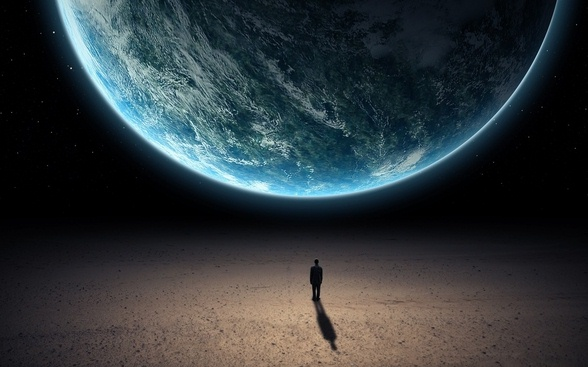
\includegraphics[scale=0.4]{Figures/World.jpg}
\caption{تصویر مفهومی}
\label{Fig:World1}
\end{figure}

نوشته نمونه نوشته نمونه نوشته نمونه نوشته نمونه نوشته نمونه نوشته نمونه نوشته نمونه نوشته نمونه نوشته نمونه نوشته نمونه نوشته نمونه نوشته نمونه نوشته نمونه نوشته نمونه نوشته نمونه نوشته نمونه نوشته نمونه نوشته نمونه نوشته نمونه نوشته نمونه نوشته نمونه نوشته نمونه.
% \MakeEnglishAbstract
% \MakeEnglishSignaturePage
% ب) از گزینه draft برای فراخوانی کلاس استفاده کنید. یعنی
% \documentclass[a4paper,fleqn,13pt,twoside,draft]{book}
% این گزینه حالت چرکنویس را ایفا می‌کند و بر روی بسته‌های مختلف اثرهای متفاوتی دارد. به‌عنوان مثال: به جای شکل، تنها چهارچوب آن نمایش داده شود، لینک‌های hyperref غیر فعال گردد، فایل‌های خارجی را در بسته listings اضافه نمی‌کند و ... و همه این موارد سبب کاهش زمان اجرا و حجم فایل می‌شود.

% در صورتی که میخواهید به سطر بعد بروید اما نمیخواهید بین دو کلمه‌ای که نوشتید فاصله بیفتد کافی است در انتهای خط اول  (بدون فاصله) کاراکتر % را اضافه کنید. با این عمل، لاتک خط فاصله ایجاد شده در اثر تغییر سطر را به عنوان توضیح اضافه یا کامنت در نظر میگیرد و در خروجی اعمال نمی‌کند.

% توصیه می‌شود از شکل‌های برداری با فرمت PDF استفاده شود. این کار علاوه بر افزایش کیفیت رسال/پایان‌نامه/گزارش، باعث کاهش حجم شکل‌ها (و در نتیجه  کاهش حجم فایل نهایی) و همچنین کاهش زمان پردازش می‌شود.

% در این قالب سعی شده است که از تمامی بخش‌های موجود در پایان‌نامه‌ها نمونه‌ای آورده شود.

\documentclass[a4paper,fleqn,11pt,oneside]{book}
\usepackage{Settings/UI-Thesis}
\usepackage[nolist]{acronym}

%-----------------------------
% دستورهای مورد نیاز را در این قسمت اضافه نمایید:
% Cross-reference commands.
\newtheorem{thm}{Theorem}[chapter]
\theoremstyle{definition}
\newtheorem{definition}[thm]{تعریف}

\newcommand{\xs}[1]{بخش~\ref{#1}}
\newcommand{\xc}[1]{فصل~\ref{#1}}
\newcommand{\xp}[1]{صفحه~\pageref{#1}}
\newcommand{\xf}[1]{شکل~\ref{#1}}
\newcommand{\xt}[1]{جدول~\ref{#1}}
\newcommand{\xa}[1]{پیوست~\ref{#1}}
\newcommand{\xd}[1]{تعریف~\ref{#1}}
\newcommand{\xr}[1]{قانون~\ref{#1}}
\newcommand{\xra}[1]{R~\ref{#1}}
\newcommand{\xl}[1]{کد~\ref{#1}}
\newcommand{\xal}[1]{الگوریتم~\ref{#1}}
\newcommand{\xe}[1]{معادله~\eqref{#1}}

\newcommand{\mylr}[1]{\texorpdfstring{\lr{#1}}{#1}}
\eqenvironment{نکات}{itemize}
\eqenvironment{تعریف}{definition}
\eqcommand{مورد}{item}

\renewcommand{\descriptionlabel}[1]%
{\hspace{\labelsep} $\checkmark$ \hspace{\labelsep}\textbf{#1}}
%%%%%%%%%%%%%%%%%%%%%%%%%%%%%%%%%%%%%%%%%%%%%%%%%%%%%%%%%%%%%%

\algnewcommand\algorithmicforeach{\textbf{for each}}
\algdef{S}[FOR]{ForEach}[1]{\algorithmicforeach\ #1\ \algorithmicdo}
%
%\algnewcommand{\IfThenElse}[3]{% \IfThenElse{<if>}{<then>}{<else>}
%  \State \algorithmicif\ #1\ \algorithmicthen\ #2\ \algorithmicelse\ #3}

\algdef{SE}[FOR]{NoDoFor}{EndFor}[1]{\algorithmicfor\ #1}{\algorithmicend\ \algorithmicfor}%
\algdef{SE}[IF]{NoThenIf}{EndIf}[1]{\algorithmicif\ #1}{\algorithmicend\ \algorithmicif}%

\newcommand*\diamondarrow{%
  \stackengine{0pt}{\hspace{1.2ex}$\rightarrow$}{$\lozenge$}{O}{l}{F}{F}{L}}
\newcommand*\fdiamondarrow{%
  \stackengine{0pt}{\hspace{1.2ex}$\rightarrow$}{$\blacklozenge$}{O}{l}{F}{F}{L}}
\newcommand*\dltriangle{%
  \stackengine{0pt}{${-}{-}$}{\hspace{3.2ex}$\vartriangleright$}{O}{l}{F}{F}{L}}
\newcommand*\ltriangle{%
  \stackengine{0pt}{${-}$\hspace{-.5ex}${-}$}{\hspace{2.8ex}$\vartriangleright$}{O}{l}{F}{F}{L}}

\makeatletter
\providecommand*{\cupdot}{%
  \mathbin{%
    \mathpalette\@cupdot{}%
  }%
}
\newcommand*{\@cupdot}[2]{%
  \ooalign{%
    $\m@th#1\cup$\cr
    \hidewidth$\m@th#1\cdot$\hidewidth
  }%
}
\makeatother

%\DeclareMathSizes{9}{9}{9}{9}

\lstset{escapeinside={/*@}{@*/}}
%\definecolor{codebackground}{rgb}{0.95,0.95,0.95}
\definecolor{codebackground}{RGB}{255,255,255}
\definecolor{commentcolor}{RGB}{77,153,153}
\definecolor{keywordcolor}{RGB}{153,77,153}
\lstset{backgroundcolor=\color{codebackground}}

\lstset{
  captionpos=b,
  numberstyle=\tiny,
  %basicstyle=\ttfamily\footnotesize,
  %basicstyle=\setLTR\thefootnotesize\ttfamily,
  basicstyle=\setLTR\bfseries\fontsize{8.5pt}{0}\selectfont\ttfamily,
  columns=flexible,
  tabsize=2,
  numbers=none, %left,
  nolol=true,
  keywordstyle=\color{keywordcolor},
  commentstyle=\color{commentcolor},
  stringstyle=\color{blue},
  captiondirection=RTL,
  upquote=true,
}

\def\lstlistingname{کد}

%\input{listings/EOLFormat}
%-----------------------------

\begin{document}

%\section*{List of Acronyms}
\begin{acronym}
\acro{MDE}{Model-Driven Engineering}
\end{acronym}

\pagestyle{plain}
\pagenumbering{harfi}
%\setcounter{page}{2}

% ░░░░░░░▒▒▒▒▒▒▓▓▓▓ In the Name of Allah ▓▓▓▓▒▒▒▒▒▒░░░░░░░
\clearpage
\thispagestyle{empty}
\newgeometry{left=3.5cm, right=3.5cm, top=3.5cm, bottom=3.5cm}
\begin{figure}
  \centering

\includegraphics[width = \linewidth]{Settings/Allah.png}
\end{figure}
% ░░░░░░░▒▒▒▒▒▒▓▓▓▓ Title Page ▓▓▓▓▒▒▒▒▒▒░░░░░░░
\DepartmentFa{دانشکده مهندسی کامپیوتر}
\GroupFa{گروه مهندسی نرم‌افزار}
\ThesisTypeFa{رساله} % Or \ThesisTypeFa{پایان‌نامه} Or \ThesisTypeFa{پیشنهادیه پایان‌نامه}
\DegreeFa{دکتری} % Or \DegreeFa{کارشناسی ارشد}
\ThesisMark{عالی} % \ThesisMark{عالی} Or \ThesisMark{بسیارخوب} Or \ThesisMark{خوب}
\FieldFa{رشته‌ی مهندسی کامپیوتر}
\BranchFa{گرایش نرم‌افزار}
\YourFullnameFa{نام و نام خانوادگی دانشجو}
\FirstSupervisorFa{نام و نام خانوادگی استاد راهنما}
% \SecondSupervisorFa{نام و نام خانوادگی استاد راهنمای دوم}
% Optional (Remove It If You Don't Have)
\YearFa{ماه سال}
\TitleFa{عنوان رساله}

% اگر عنوان رساله طولانی بود، در دو خط به صورت نشان داده شده تقسیم شود.
%\TitleFa{قسمت اول عنوان \\ [0.4cm] قسمت دوم عنوان}

\MakeTitlePage

% ░░░░░░░▒▒▒▒▒▒▓▓▓▓ CopyRight ▓▓▓▓▒▒▒▒▒▒░░░░░░░
\MakeCopyRightPage

% ░░░░░░░▒▒▒▒▒▒▓▓▓▓ Signature - Farsi ▓▓▓▓▒▒▒▒▒▒░░░░░░░
\Prefix{آقای} %\Prefix{خانم}
\DateFa{1396/06/11}
\FirstSupervisorAcademicRank{استادیار} % Or \FirstSupervisorAcademicRank{دانشیار} Or \FirstSupervisorAcademicRank{استاد}
% \SecondSupervisorAcademicRank{استادیار} % Or \SecondSupervisorAcademicRank{دانشیار} Or \SecondSupervisorAcademicRank{استاد}
%\FirstAdvisorFa{مشاور اول}
%\FirstAdvisorAcademicRank{استادیار} % Or \FirstAdvisorAcademicRank{دانشیار} Or \FirstAdvisorAcademicRank{استاد}
%\SecondAdvisorFa{مشاور دوم} % Optional (Remove It If You Don't Have)
%\SecondAdvisorAcademicRank{استادیار} % Or \SecondAdvisorAcademicRank{دانشیار} Or \SecondAdvisorAcademicRank{استاد}
\FirstExaminerFa{نام و نام خانوادگی داور اول داخلی}
\FirstExaminerAcademicRank{مرتبه علمی} % Or \FirstExaminerAcademicRank{دانشیار} Or \FirstExaminerAcademicRank{استاد}
\SecondExaminerFa{نام و نام خانوادگی استاد داور دوم داخلی} % Optional (Remove It If You Don't Have)
\SecondExaminerAcademicRank{مرتبه علمی} % Or \SecondExaminerAcademicRank{دانشیار} Or \SecondExaminerAcademicRank{استاد}
\ThirdExaminerFa{نام و نام خانوادگی داور خارج} % Optional (Remove It If You Don't Have)
\ThirdExaminerAcademicRank{مرتبه علمی} % Or \SecondExaminerAcademicRank{دانشیار} Or \SecondExaminerAcademicRank{استاد}
%\DeanOfDepartmentFa{دکتر تحصیلات تکمیلی دانشکده}

\MakeFarsiSignaturePage

% ░░░░░░░▒▒▒▒▒▒▓▓▓▓ Acknowledgments ▓▓▓▓▒▒▒▒▒▒░░░░░░░
% !TEX root = ../ui-thesis.tex
% !TeX program = xelatex

\clearpage
\thispagestyle{empty}
\newgeometry{left=3.5cm,right=3.5cm,top=7cm}

{\BNazaninScaleOne
{\fontsize{20pt}{0}\selectfont \bfseries
\noindent
% عنوان تشکر و قدردانی---------------------------------------------------------
سپاس‌گزاری
% ؛---------------------------------------------------------
}}
\vspace{0.5cm}

{\BNazaninScaleOne
{\fontsize{12pt}{0.9cm}\selectfont % ‌B Nazanin 13
\noindent
% متن تشکر و قدردانی---------------------------------------------------------
خدایا تو را شاکرم به خاطر امروزم که به من عطا فرمودی...






% ؛---------------------------------------------------------
}}

\restoregeometry

% ░░░░░░░▒▒▒▒▒▒▓▓▓▓ Dedication ▓▓▓▓▒▒▒▒▒▒░░░░░░░
\clearpage
\thispagestyle{empty}
\newgeometry{left=3.5cm,right=3.5cm,top=7cm}

{\BNazaninScaleOne
{\fontsize{20pt}{0}\selectfont \bfseries
\noindent
% تقدیم اثر---------------------------------------------------------
تقدیم به
\\[1cm]
\hspace*{1cm}
............................
% ؛---------------------------------------------------------
}}
		
\restoregeometry

% ░░░░░░░▒▒▒▒▒▒▓▓▓▓ Abstract - Farsi ▓▓▓▓▒▒▒▒▒▒░░░░░░░
\AbstractFa{
در این قسمت چکیده‌ی فارسی پایان‌نامه نوشته می‌شود. در این قسمت چکیده‌ی فارسی پایان‌نامه نوشته می‌شود. در این قسمت چکیده‌ی فارسی پایان‌نامه نوشته می‌شود. در این قسمت چکیده‌ی فارسی پایان‌نامه نوشته می‌شود. در این قسمت چکیده‌ی فارسی پایان‌نامه نوشته می‌شود. در این قسمت چکیده‌ی فارسی پایان‌نامه نوشته می‌شود. در این قسمت چکیده‌ی فارسی پایان‌نامه نوشته می‌شود. در این قسمت چکیده‌ی فارسی پایان‌نامه نوشته می‌شود. در این قسمت چکیده‌ی فارسی پایان‌نامه نوشته می‌شود. در این قسمت چکیده‌ی فارسی پایان‌نامه نوشته می‌شود. در این قسمت چکیده‌ی فارسی پایان‌نامه نوشته می‌شود. در این قسمت چکیده‌ی فارسی پایان‌نامه نوشته می‌شود. در این قسمت چکیده‌ی فارسی پایان‌نامه نوشته می‌شود. در این قسمت چکیده‌ی فارسی پایان‌نامه نوشته می‌شود. در این قسمت چکیده‌ی فارسی پایان‌نامه نوشته می‌شود. در این قسمت چکیده‌ی فارسی پایان‌نامه نوشته می‌شود. در این قسمت چکیده‌ی فارسی پایان‌نامه نوشته می‌شود. در این قسمت چکیده‌ی فارسی پایان‌نامه نوشته می‌شود. در این قسمت چکیده‌ی فارسی پایان‌نامه نوشته می‌شود. در این قسمت چکیده‌ی فارسی پایان‌نامه نوشته می‌شود. در این قسمت چکیده‌ی فارسی پایان‌نامه نوشته می‌شود. در این قسمت چکیده‌ی فارسی پایان‌نامه نوشته می‌شود. در این قسمت چکیده‌ی فارسی پایان‌نامه نوشته می‌شود. در این قسمت چکیده‌ی فارسی پایان‌نامه نوشته می‌شود. در این قسمت چکیده‌ی فارسی پایان‌نامه نوشته می‌شود. در این قسمت چکیده‌ی فارسی پایان‌نامه نوشته می‌شود. در این قسمت چکیده‌ی فارسی پایان‌نامه نوشته می‌شود. در این قسمت چکیده‌ی فارسی پایان‌نامه نوشته می‌شود. در این قسمت چکیده‌ی فارسی پایان‌نامه نوشته می‌شود. در این قسمت چکیده‌ی فارسی پایان‌نامه نوشته می‌شود.‎‎
}

\KeywordsFa{
1-کلمه‌ی کليدی اوّل،  2-کلمه‌ی کليدی دوم ، 3-کلمه‌ی کليدی سوم،  4-کلمه‌ی کليدی چهارم، 5-کلمه‌ی کليدی پنجم
}
\MakeFarsiAbstract

% ░░░░░░░▒▒▒▒▒▒▓▓▓▓ Table of Contents/Figures/Tables ▓▓▓▓▒▒▒▒▒▒░░░░░░░
\setcounter{page}{0}
\MakeTableOfContents
\MakeListOfFigures
\MakeListOfTables

% ----------------------------------------------------------------------------
\clearpage
\pagestyle{myheadings}
\pagenumbering{arabic}
\setcounter{page}{1}

% ░░░░░░░▒▒▒▒▒▒▓▓▓▓ Chapters ▓▓▓▓▒▒▒▒▒▒░░░░░░░
\clearpage
\baselineskip=0.9cm

% !TEX root = ../ui-thesis.tex
% !TeX program = xelatex

\chapter{مقدمه}
\section{پیش‌گفتار}
این نمونه‌ای از زیرنویس \LTRfootnote{English Footnote} انگلیسی است.	
این نمونه‌ای از زیرنویس \LTRfootnote{English Footnote} انگلیسی است.	
در این قالب سعی شده است که از تمامی بخش‌های موجود در پایان‌نامه‌ها نمونه‌ای آورده شود. در این قالب سعی شده است که از تمامی بخش‌های موجود در پایان‌نامه‌ها نمونه‌ای آورده شود. در این قالب سعی شده است که از تمامی بخش‌های موجود در پایان‌نامه‌ها نمونه‌ای آورده شود. در این قالب سعی شده است که از تمامی بخش‌های موجود در پایان‌نامه‌ها نمونه‌ای آورده شود. در این قالب سعی شده است که از تمامی بخش‌های موجود در پایان‌نامه‌ها نمونه‌ای آورده شود. در این قالب سعی شده است که از تمامی بخش‌های موجود در پایان‌نامه‌ها نمونه‌ای آورده شود. در این قالب سعی شده است که از تمامی بخش‌های موجود در پایان‌نامه‌ها نمونه‌ای آورده شود. در این قالب سعی شده است که از تمامی بخش‌های موجود در پایان‌نامه‌ها نمونه‌ای آورده شود. در این قالب سعی شده است که از تمامی بخش‌های موجود در پایان‌نامه‌ها نمونه‌ای آورده شود. در این قالب سعی شده است که از تمامی بخش‌های موجود در پایان‌نامه‌ها نمونه‌ای آورده شود. در این قالب سعی شده است که از تمامی بخش‌های موجود در پایان‌نامه‌ها نمونه‌ای آورده شود. در این قالب سعی شده است که از تمامی بخش‌های موجود در پایان‌نامه‌ها نمونه‌ای آورده شود. در این قالب سعی شده است که از تمامی بخش‌های موجود در پایان‌نامه‌ها نمونه‌ای آورده شود. در این قالب سعی شده است که از تمامی بخش‌های موجود در پایان‌نامه‌ها نمونه‌ای آورده شود.
\section{بخش اول}
نمونه‌ای از یک عبارت انگلیسی در متن به‌صورت

\lr{English Sentence}
است. نمونه‌ای از یک عبارت ریاضی در متن نیز به‌صورت
$x^2 + y^2$
است. ارجاع به مراجع انگلیسی
\cite{Fakhari2015a,Lewis2003}.
ارجاع به مراجع فارسی
\cite{Fakhari2015b,HadianThesis2008}.
این نمونه‌ای از یک زیرنویس انگلیسی%
\LTRfootnote{English Footnote}
است. این نمونه‌ای از یک زیرنویس فارسی%
\RTLfootnote{زیرنویس فارسی}
است. در شکل
\ref{Fig:SampleFigure1}،
نمونه‌ای از یک شکل آورده شده است. 

\begin{figure}[!htb]
\centering
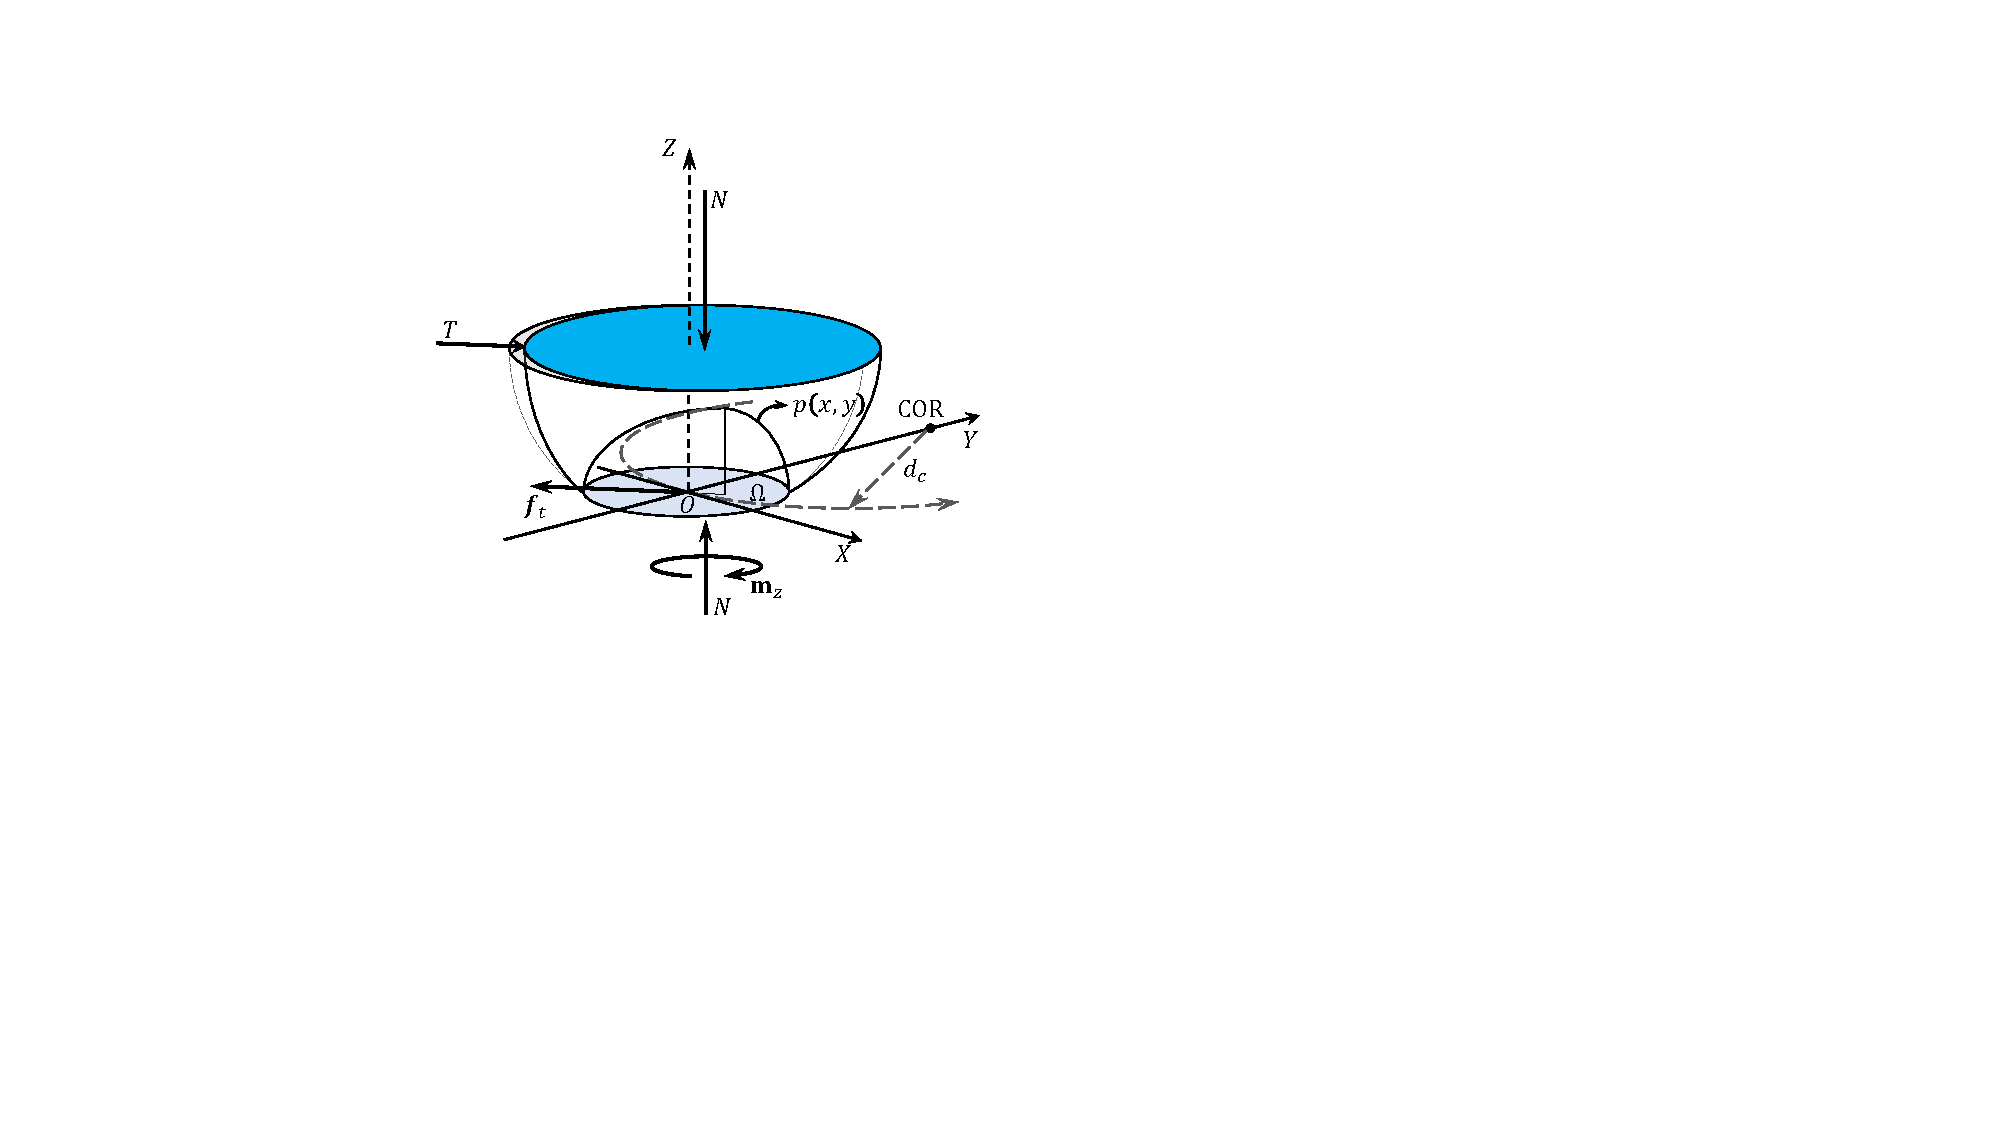
\includegraphics[scale=1]{Figures/SampleFigure.pdf}
\caption{شکل نمونه}
\label{Fig:SampleFigure1}
\end{figure}

نمونه‌ای از قرار دادن دو شکل در کنار یکدیگر در شکل
\ref{Fig:SampleFigure2}
آورده شده است.

\begin{figure}[!htb]
\centering
\subfloat[زیرنویس شکل اول]{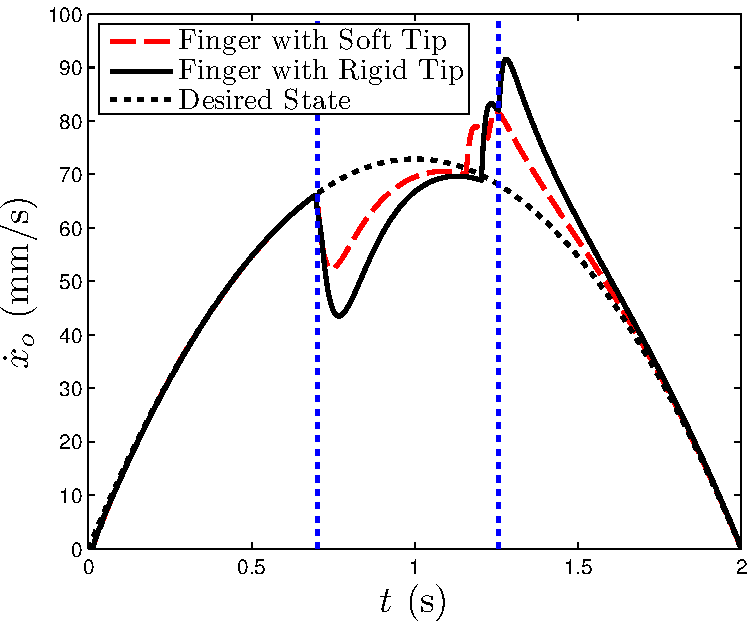
\includegraphics[scale=0.56]{Figures/FigureA.pdf}}
\quad
\subfloat[زیرنویس شکل دوم]{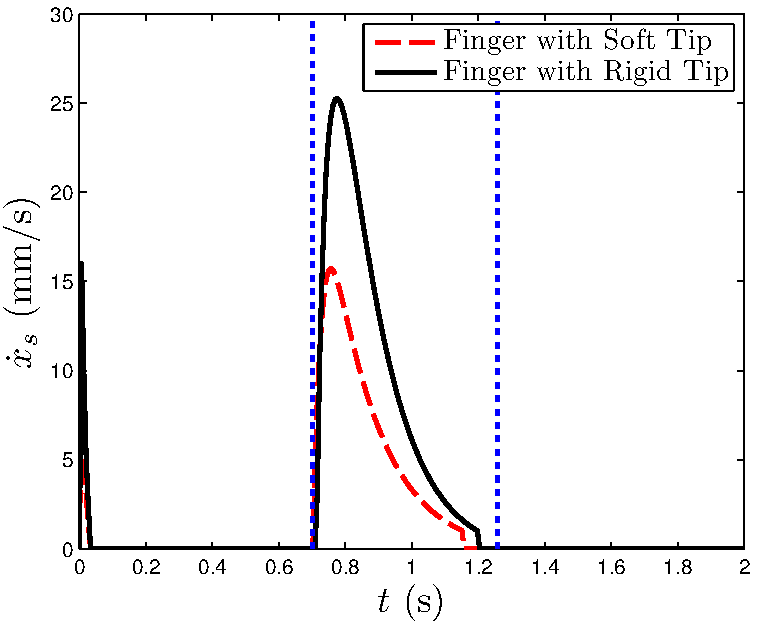
\includegraphics[scale=0.56]{Figures/FigureB.pdf}}
\caption{
قرار دادن دو شکل در کنار یکدیگر، الف) شکل نمونه اول،
ب) شکل نمونه دوم
}
\label{Fig:SampleFigure2}
\end{figure}





آیتم‌های مختلف به‌صورت زیر آورده می‌شود:
\begin{itemize}[label=-]
\item
مورد اول
\item
مورد دوم
\item
مورد سوم
\end{itemize}

نمونه‌ای از آیتم‌های شماره‌دار نیز در ادامه آورده شده است. به طور کلی معماری برداشت انرژی به دو دسته‌ی کلی تقسیم می‌شود:
\begin{enumerate}[label=\arabic*)]
\item
برداشت-استفاده:

در این حالت سیستم بلافاصله انرژی برداشت‌شده را مصرف می‌کند. واضح است اگر انرژی کافی در محیط وجود نداشته باشد دستگاه از کار می‌افتد. این نوع سیستم‌ها بیشتر در فشار دادن کلید‌ها، پدال‌ها و دستگاه‌های ردیابی برای انسان‌ها استفاده می‌شود. به طور مثال در پاشنه‌ی کفش دونده‌ای مواد پیزوالکتریک کار گذاشته می‌شود و با فشار پا بر روی کفش و فشرده شدن پیزوالکتریک داخل کفش، انرژی الکتریکی برای ارسال سیگنال 
\lr{RF}
و در نتیجه ردیابی دونده تامین می‌شود. 
\item
برداشت-ذخیره-استفاده:

در این روش سیستم برای ذخیره‌ی انرژی برداشت‌شده به باتری مجهز شده است. این روش برای زمانی‌که انرژی زیادی در محیط وجود داشته باشد و برای منابعی مانند انرژی خورشیدی  کاربرد دارد. روش‌های زیادی برای تبدیل انرژی خورشیدی به انرژی الکتریکی از جمله سلول‌های خورشیدی وجود دارد. در این حالت چگونگی ذخیره‌ی انرژی و بهینه‌سازی مصرف انرژی مطرح می‌شود.
\end{enumerate}




\subsection{زیربخش اول}
لورم ایپسوم متن ساختگی با تولید سادگی نامفهوم از صنعت چاپ و با استفاده از طراحان گرافیک است. چاپگرها و متون بلکه روزنامه و مجله در ستون و سطرآنچنان که لازم است و برای شرایط فعلی تکنولوژی مورد نیاز و کاربردهای متنوع با هدف بهبود ابزارهای کاربردی می باشد. کتابهای زیادی در شصت و سه درصد گذشته، حال و آینده شناخت فراوان جامعه و متخصصان را می طلبد تا با نرم افزارها شناخت بیشتری را برای طراحان رایانه ای علی الخصوص طراحان خلاقی و فرهنگ پیشرو در زبان فارسی ایجاد کرد. در این صورت می توان امید داشت که تمام و دشواری موجود در ارائه راهکارها و شرایط سخت تایپ به پایان رسد وزمان مورد نیاز شامل حروفچینی دستاوردهای اصلی و جوابگوی سوالات پیوسته اهل دنیای موجود طراحی اساسا مورد استفاده قرار گیرد. در جدول
\ref{Tbl:SampleTable1}،
نمونه‌ای از یک جدول واردشده در لاتک و در جدول
\ref{Tbl:SampleTable2}،
نمونه‌ای از یک جدول نوشته‌شده در لاتک آورده شده است.

\begin{table}[!htb]
\caption{پارامترهای شبیه‌سازی}
\centering
\begin{tabular}{c}
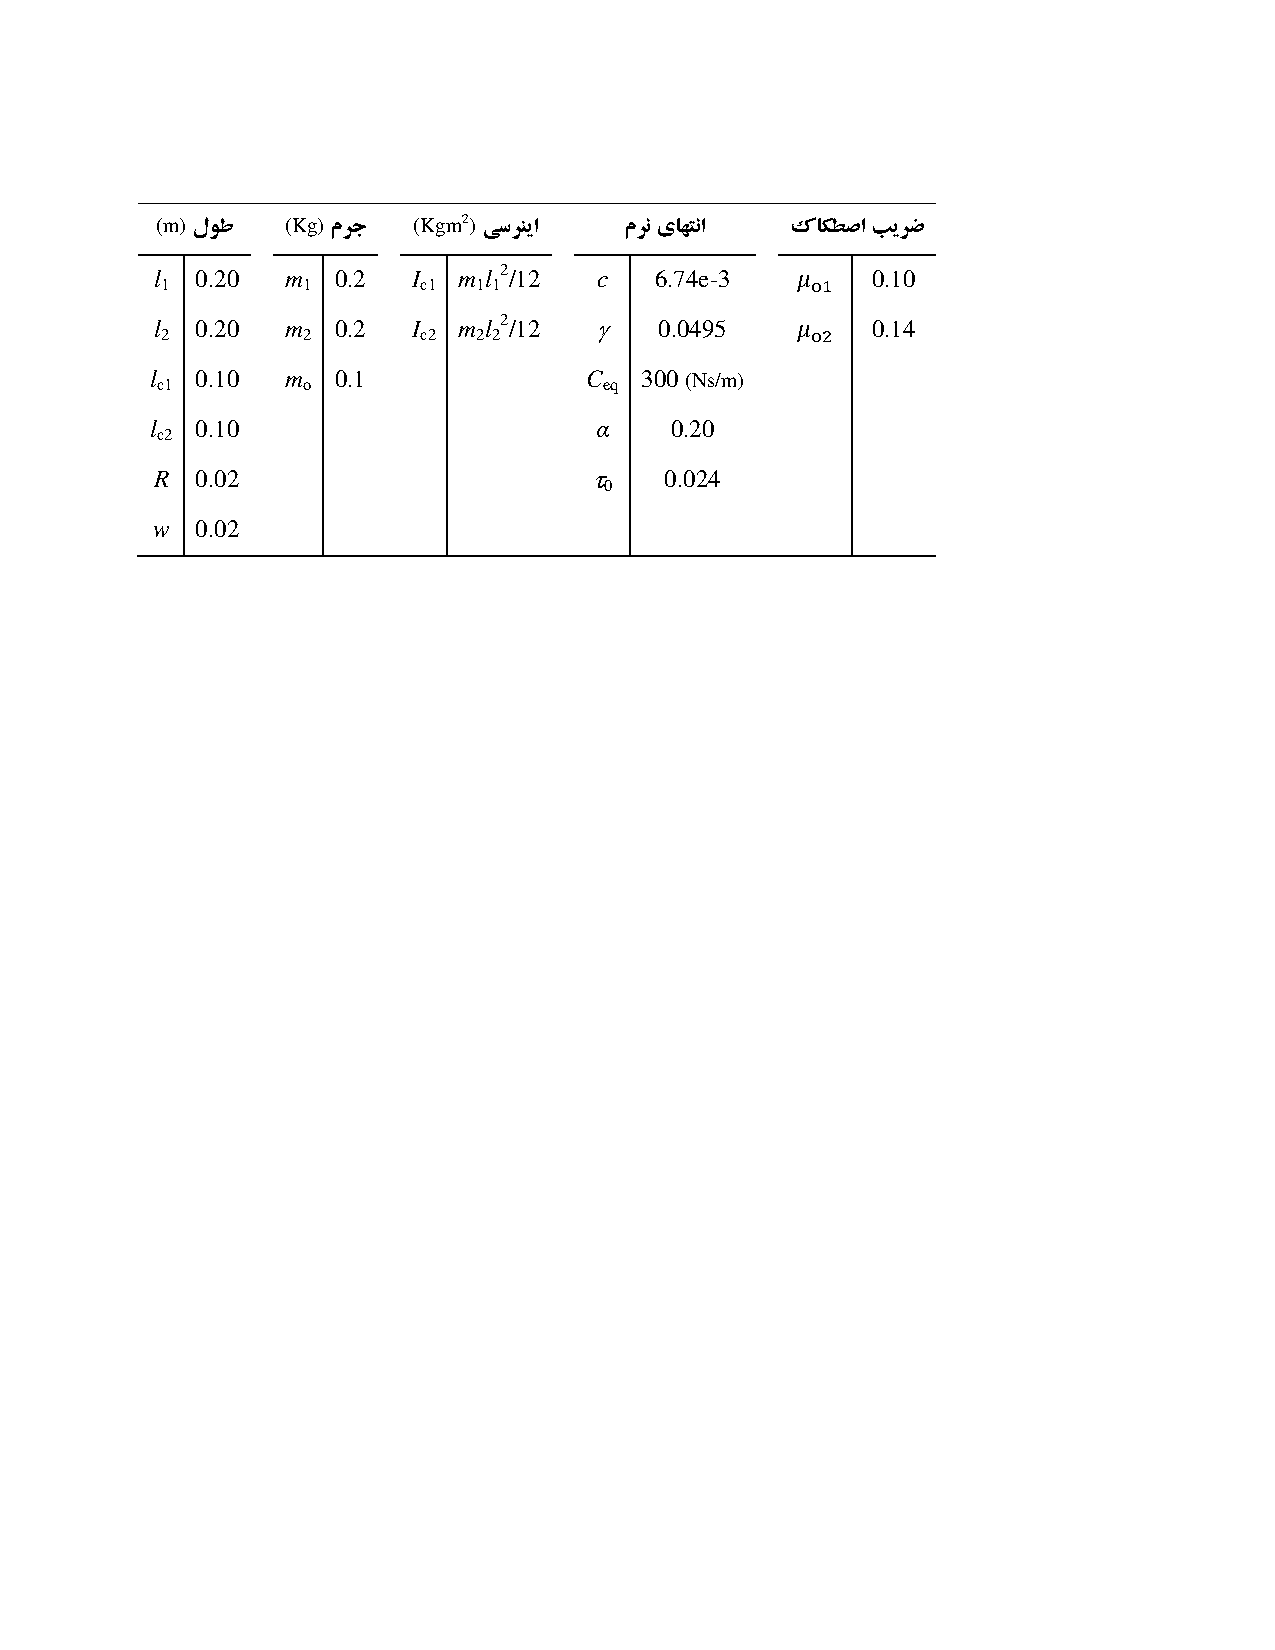
\includegraphics[scale=0.9]{Figures/SampleTable1.pdf} 
\end{tabular}
\vspace{-\baselineskip}
\label{Tbl:SampleTable1}
\end{table}

\begin{table}[!htb]
\caption{مقايسه‌ی روش‌هاي برداشت انرژي مبتني بر لرزش‌هاي مکانيکی}
\centering
\begin{tabular}{@{}|p{.15\textwidth}|p{.25\textwidth}|p{.25\textwidth}|p{.25\textwidth}|@{}}
\hline
روش
& 
چگالی انرژی
& 
ابعاد
& 
عیب اصلی
\\ \hline \hline
پیزوالکتریک
& 
$\mathrm{mJ/cm^3}$ 35/4
& 
بزرگ
& 
ولتاژ خروجی کم
\\ \hline
الکترومغناطیس
& 
$\mathrm{mJ/cm^3}$ 24/8
& 
بزرگ
& 
ولتاژ خروجی بسیار کم
\\ \hline
الکترواستاتیک
& 
$\mathrm{mJ/cm^3}$ 4
& 
فشرده در تراشه‌ها
& 
نیاز به منبع شارژ اولیه
\\ \hline
\end{tabular}
\label{Tbl:SampleTable2}
\vspace{-\baselineskip}
\end{table}

نمونه‌ای از یک رابطه به‌صورت
\begin{equation}
p\left( r \right) = {C_k}\frac{N}{{\pi {a^2}}}{\left[{1 - {{\left( {\frac{r}{a}} \right)}^k}} \right]^{\frac{1}{k}}},
\label{Eq:Pressure}
\end{equation}
است. در رابطه
\ref{Eq:Pressure}،
$N$
نیروی عمودی است. نمونه‌ای از استفاده از روابط متوالی به‌صورت
\begin{equation}
\sum \limits_{i = 1}^{k + 1} {E_s}\left( i \right) - T \sum \limits_{i = 1}^k {P_s}\left( i \right) \le B_s^{max},\quad k = 1, \ldots ,N - 1,
\label{Eq:batterysource}
\end{equation}\vspace{-\baselineskip}
\begin{equation}
\sum \limits_{i = 1}^{k + 1} {E_r}\left( i \right) - T \sum \limits_{i = 1}^k {P_r}\left( i \right) \le B_r^{max},\quad k = 1, \ldots ,N - 1,
\label{Eq:batteryrellay}
\end{equation}
است. نمونه‌ای از یک قضیه و تبصره نیز در ادامه آورده شده است.
\begin{theorem}
اگر ظرفیت باتری‌ها به اندازه کافی بزرگ باشد، جواب بهینه‌ی 
$P_s^*(i)$
و
$P_r^*(i)$
وجود دارد به نحوی که تابع هدف را بیشینه می‌کند و در رابطه‌ی زیر صدق می‌کند:
\begin{equation}
C\left( {{{\left| {{h_{sr}}\left( i \right)} \right|}^2}{P_s}^*\left( i \right)} \right) \ge C\left( {{{\left| {{h_{sd}}\left( i \right)} \right|}^2}{P_s}^*\left( i \right)} \right) + C\left( {{{\left| {{h_{rd}}\left( {i + 1} \right)} \right|}^2}P_r^*\left( {i} \right)} \right).
\label{Eq:theorem1}
\end{equation}

\begin{proof}
بار دیگر فرم تابع هدف را در نظر می‌گیریم. لازم به ذکر است اینجا تابع هدف یک تابع دومتغیره است.
\begin{equation}
{R({\mathbf{P}_s},{\mathbf{P}_r}) = {\frac{1}{2}\sum\limits_{i = 1}^N {\min } \left\{ {C\left( {{{\left| {{h_{sr}}\left( i \right)} \right|}^2}{P_s}\left( i \right)} \right),} C\left( {{{\left| {{h_{sd}}\left( i \right)} \right|}^2}{P_s}\left( i \right)} \right) \right\} }}.
\end{equation}
حال بلوک
$i$ام
را در نظر می‌گیریم. اگر رابطه‌ی
\ref{Eq:theorem1}
برای
$i$
برقرار نباشد، به عبارت دیگر اگر داشته باشیم،
\begin{equation}
C\left( {{{\left| {{h_{sr}}\left( i \right)} \right|}^2}{P_s}^*\left( i \right)} \right) < C\left( {{{\left| {{h_{sd}}\left( i \right)} \right|}^2}{P_s}^*\left( i \right)} \right) + C\left( {{{\left| {{h_{rd}}\left( {i + 1} \right)} \right|}^2}P_r^*\left( {i + 1} \right)} \right),
\label{Eq:theorem1(2)}
\end{equation}
بنابراین
\begin{equation}
C\left( {{{\left| {{h_{sr}}\left( i \right)} \right|}^2}{P_s}^*\left( i \right)} \right)+ C\left( {{{\left| {{h_{sd}}\left( i \right)} \right|}^2}{P_s}^*\left( i \right)} \right) =C\left( {{{\left| {{h_{sr}}\left( i \right)} \right|}^2}{P_s}^*\left( i \right)} \right).
\end{equation}
پس در تابع هدف مسئله، مقدار بهینه‌ی مسئله برابر عبارت سمت چپ رابطه‌ی
\ref{Eq:theorem1(2)}
شده است و آرگومان دوم و  هم‌چنین مقدار
$P_r^*(i)$
هیچ نقشی در مقدار بهینه ندارد. بنابراین می‌توانیم 
$P_r^*(i)$
را آنقدر کاهش دهیم تا در رابطه‌ی
\ref{Eq:theorem1(2)}
تساوی برقرار شود بدون آنکه مقدار بهینه‌ی مسئله تغییر کند.
\end{proof}
\label{theorem1}
\end{theorem}

\begin{remark}
از قضیه‌ی
\ref{theorem1}
نتیجه می‌گیریم که جواب بهینه‌ی مسئله‌ی
\lr{P}
در حالت کلی یکتا نیست. به طور مثال وقتی مقدار انرژی برداشت‌شده در رله خیلی بیشتر از این انرژی در منبع باشد مسئله می‌تواند جواب‌های زیادی داشته باشد. بنابراین همواره می‌توان برای صرفه‌جویی در مصرف انرژی، بدون کاهش مقدار نرخ گذردهی سیستم، کمترین مقدار توان را برای رله انتخاب کرد. بنابراین با توجه به رابطه
\begin{equation}
C\left( {{{\left| {{h_{sr}}\left( i \right)} \right|}^2}{P_s}^*\left( i \right)} \right) 
\ge C\left( {{{\left| {{h_{sd}}\left( i \right)} \right|}^2}{P_s}^*\left( i \right)} \right) + C\left( {{{\left| {{h_{rd}}\left( {i} \right)} \right|}^2}P_r^*\left( {i} \right)} \right),
\label{Eq:remark1}
\end{equation}
و با  استفاده از رابطه
\ref{Eq:remark1}
خواهیم داشت،
\begin{equation}
{R_r}(i) = \min \left\{ {C\left( {{{\left| {{h_{rd}}(i)} \right|}^2}{P_r}(i)} \right),C\left( {{{\left| {{h_{sr}}(i)} \right|}^2}{P_s}(i)} \right)} \right\}.
\end{equation}

بنابراین می‌توان با انتخاب کمترین توان و نرخ برای رله از مصرف بی‌رویه‌ی انرژی جلوگیری کرد. فرض بزرگ بودن ظرفیت باتری‌ به این دلیل است که اگر ظرفیت باتری محدود باشد برای کاهش
$P_r^*(i)$
با محدودیت مواجه هستیم. چون در صورت کاهش بی از حد توان رله ممکن است از ناحیه‌ی شدنی مسئله خارج شویم. به هر حال برای هر دو حالت ظرفیت نامحدود و محدود باتری جواب مسئله یکتا نیست و همواره می‌توان با کاهش توان رله مصرف انرژی را کاهش داد.
\end{remark}

\section{نام بخش همراه با کلمه انگلیسی
 \mylr{Some English Words} در آن}





%\chapter{مطالب اصلی}
\section{پیش‌گفتار}
در این قالب سعی شده است که از تمامی بخش‌های موجود در پایان‌نامه‌ها نمونه‌ای آورده شود. در این قالب سعی شده است که از تمامی بخش‌های موجود در پایان‌نامه‌ها نمونه‌ای آورده شود. در این قالب سعی شده است که از تمامی بخش‌های موجود در پایان‌نامه‌ها نمونه‌ای آورده شود. در این قالب سعی شده است که از تمامی بخش‌های موجود در پایان‌نامه‌ها نمونه‌ای آورده شود. در این قالب سعی شده است که از تمامی بخش‌های موجود در پایان‌نامه‌ها نمونه‌ای آورده شود. در این قالب سعی شده است که از تمامی بخش‌های موجود در پایان‌نامه‌ها نمونه‌ای آورده شود. در این قالب سعی شده است که از تمامی بخش‌های موجود در پایان‌نامه‌ها نمونه‌ای آورده شود. در این قالب سعی شده است که از تمامی بخش‌های موجود در پایان‌نامه‌ها نمونه‌ای آورده شود. در این قالب سعی شده است که از تمامی بخش‌های موجود در پایان‌نامه‌ها نمونه‌ای آورده شود. در این قالب سعی شده است که از تمامی بخش‌های موجود در پایان‌نامه‌ها نمونه‌ای آورده شود. در این قالب سعی شده است که از تمامی بخش‌های موجود در پایان‌نامه‌ها نمونه‌ای آورده شود. در این قالب سعی شده است که از تمامی بخش‌های موجود در پایان‌نامه‌ها نمونه‌ای آورده شود. در این قالب سعی شده است که از تمامی بخش‌های موجود در پایان‌نامه‌ها نمونه‌ای آورده شود. در این قالب سعی شده است که از تمامی بخش‌های موجود در پایان‌نامه‌ها نمونه‌ای آورده شود.
\section{بخش اول}
نمونه‌ای از یک عبارت انگلیسی در متن به‌صورت
\lr{English Sentence}
است. نمونه‌ای از یک عبارت ریاضی در متن نیز به‌صورت
$x^2 + y^2$
است. ارجاع به مراجع انگلیسی
\cite{Fakhari2015a,Lewis2003}.
ارجاع به مراجع فارسی
\cite{Fakhari2015b,HadianThesis2008}.
این نمونه‌ای از یک زیرنویس انگلیسی%
\LTRfootnote{English Footnote}
است. این نمونه‌ای از یک زیرنویس فارسی%
\RTLfootnote{زیرنویس فارسی}
است. در شکل
\ref{Fig:SampleFigure1_2}،
نمونه‌ای از یک شکل آورده شده است. 

\begin{figure}[!htb]
\centering
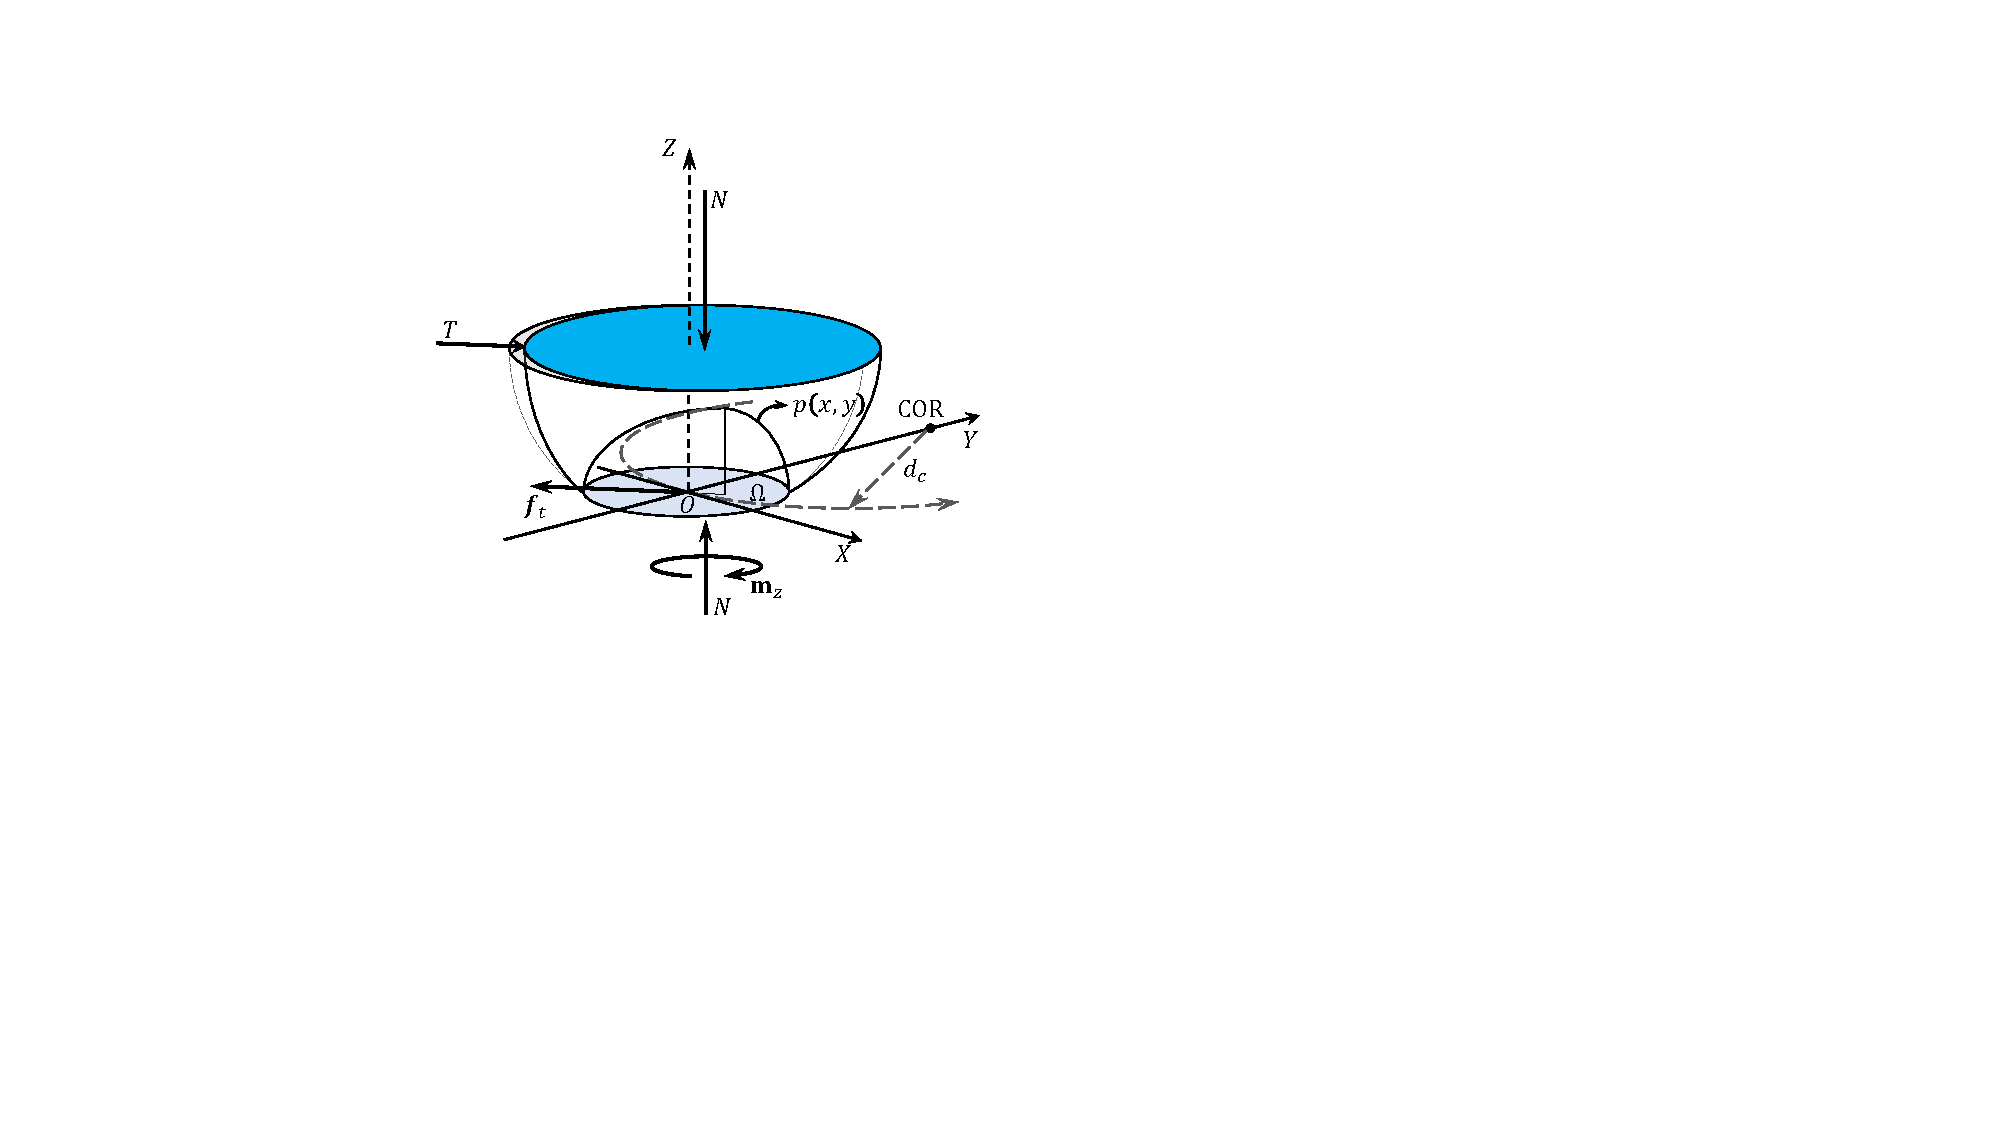
\includegraphics[scale=1]{Figures/SampleFigure.pdf}
\caption{شکل نمونه}
\label{Fig:SampleFigure1_2}
\end{figure}

نمونه‌ای از قرار دادن دو شکل در کنار یکدیگر در شکل
\ref{Fig:SampleFigure2_2}
آورده شده است.

\begin{figure}[!htb]
\centering
\subfloat[زیرنویس شکل اول]{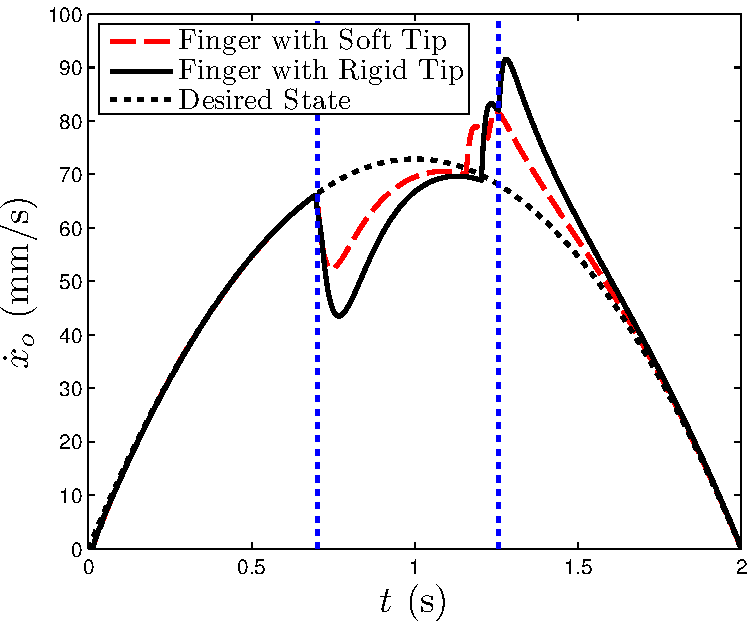
\includegraphics[scale=0.56]{Figures/FigureA.pdf}}
\quad
\subfloat[زیرنویس شکل دوم]{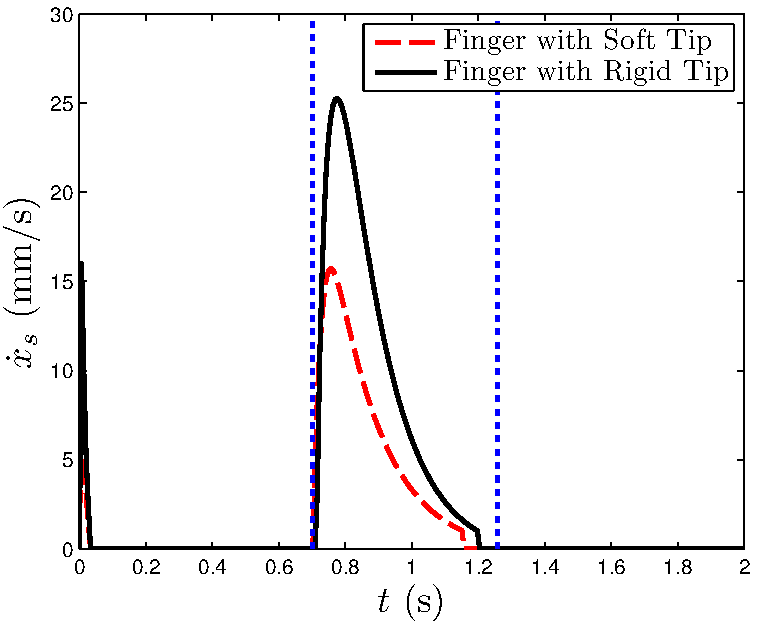
\includegraphics[scale=0.56]{Figures/FigureB.pdf}}
\caption{
قرار دادن دو شکل در کنار یکدیگر، الف) شکل نمونه اول،
ب) شکل نمونه دوم
}
\label{Fig:SampleFigure2_2}
\end{figure}





آیتم‌های مختلف به‌صورت زیر آورده می‌شود:
\begin{itemize}[label=-]
\item
مورد اول
\item
مورد دوم
\item
مورد سوم
\end{itemize}

نمونه‌ای از آیتم‌های شماره‌دار نیز در ادامه آورده شده است. به طور کلی معماری برداشت انرژی به دو دسته‌ی کلی تقسیم می‌شود:
\begin{enumerate}[label=\arabic*)]
\item
برداشت-استفاده:

در این حالت سیستم بلافاصله انرژی برداشت‌شده را مصرف می‌کند. واضح است اگر انرژی کافی در محیط وجود نداشته باشد دستگاه از کار می‌افتد. این نوع سیستم‌ها بیشتر در فشار دادن کلید‌ها، پدال‌ها و دستگاه‌های ردیابی برای انسان‌ها استفاده می‌شود. به طور مثال در پاشنه‌ی کفش دونده‌ای مواد پیزوالکتریک کار گذاشته می‌شود و با فشار پا بر روی کفش و فشرده شدن پیزوالکتریک داخل کفش، انرژی الکتریکی برای ارسال سیگنال 
\lr{RF}
و در نتیجه ردیابی دونده تامین می‌شود. 
\item
برداشت-ذخیره-استفاده:

در این روش سیستم برای ذخیره‌ی انرژی برداشت‌شده به باتری مجهز شده است. این روش برای زمانی‌که انرژی زیادی در محیط وجود داشته باشد و برای منابعی مانند انرژی خورشیدی  کاربرد دارد. روش‌های زیادی برای تبدیل انرژی خورشیدی به انرژی الکتریکی از جمله سلول‌های خورشیدی وجود دارد. در این حالت چگونگی ذخیره‌ی انرژی و بهینه‌سازی مصرف انرژی مطرح می‌شود.
\end{enumerate}




\subsection{زیربخش اول}
نوشته نمونه نوشته نمونه نوشته نمونه نوشته نمونه نوشته نمونه نوشته نمونه نوشته نمونه نوشته نمونه نوشته نمونه نوشته نمونه نوشته نمونه نوشته نمونه نوشته نمونه نوشته نمونه نوشته نمونه نوشته نمونه نوشته نمونه نوشته نمونه نوشته نمونه نوشته نمونه نوشته نمونه نوشته نمونه. در جدول
\ref{Tbl:SampleTable1_2}،
نمونه‌ای از یک جدول واردشده در لاتک و در جدول
\ref{Tbl:SampleTable2_2}،
نمونه‌ای از یک جدول نوشته‌شده در لاتک آورده شده است.

\begin{table}[!htb]
\caption{پارامترهای شبیه‌سازی}
\centering
\begin{tabular}{c}
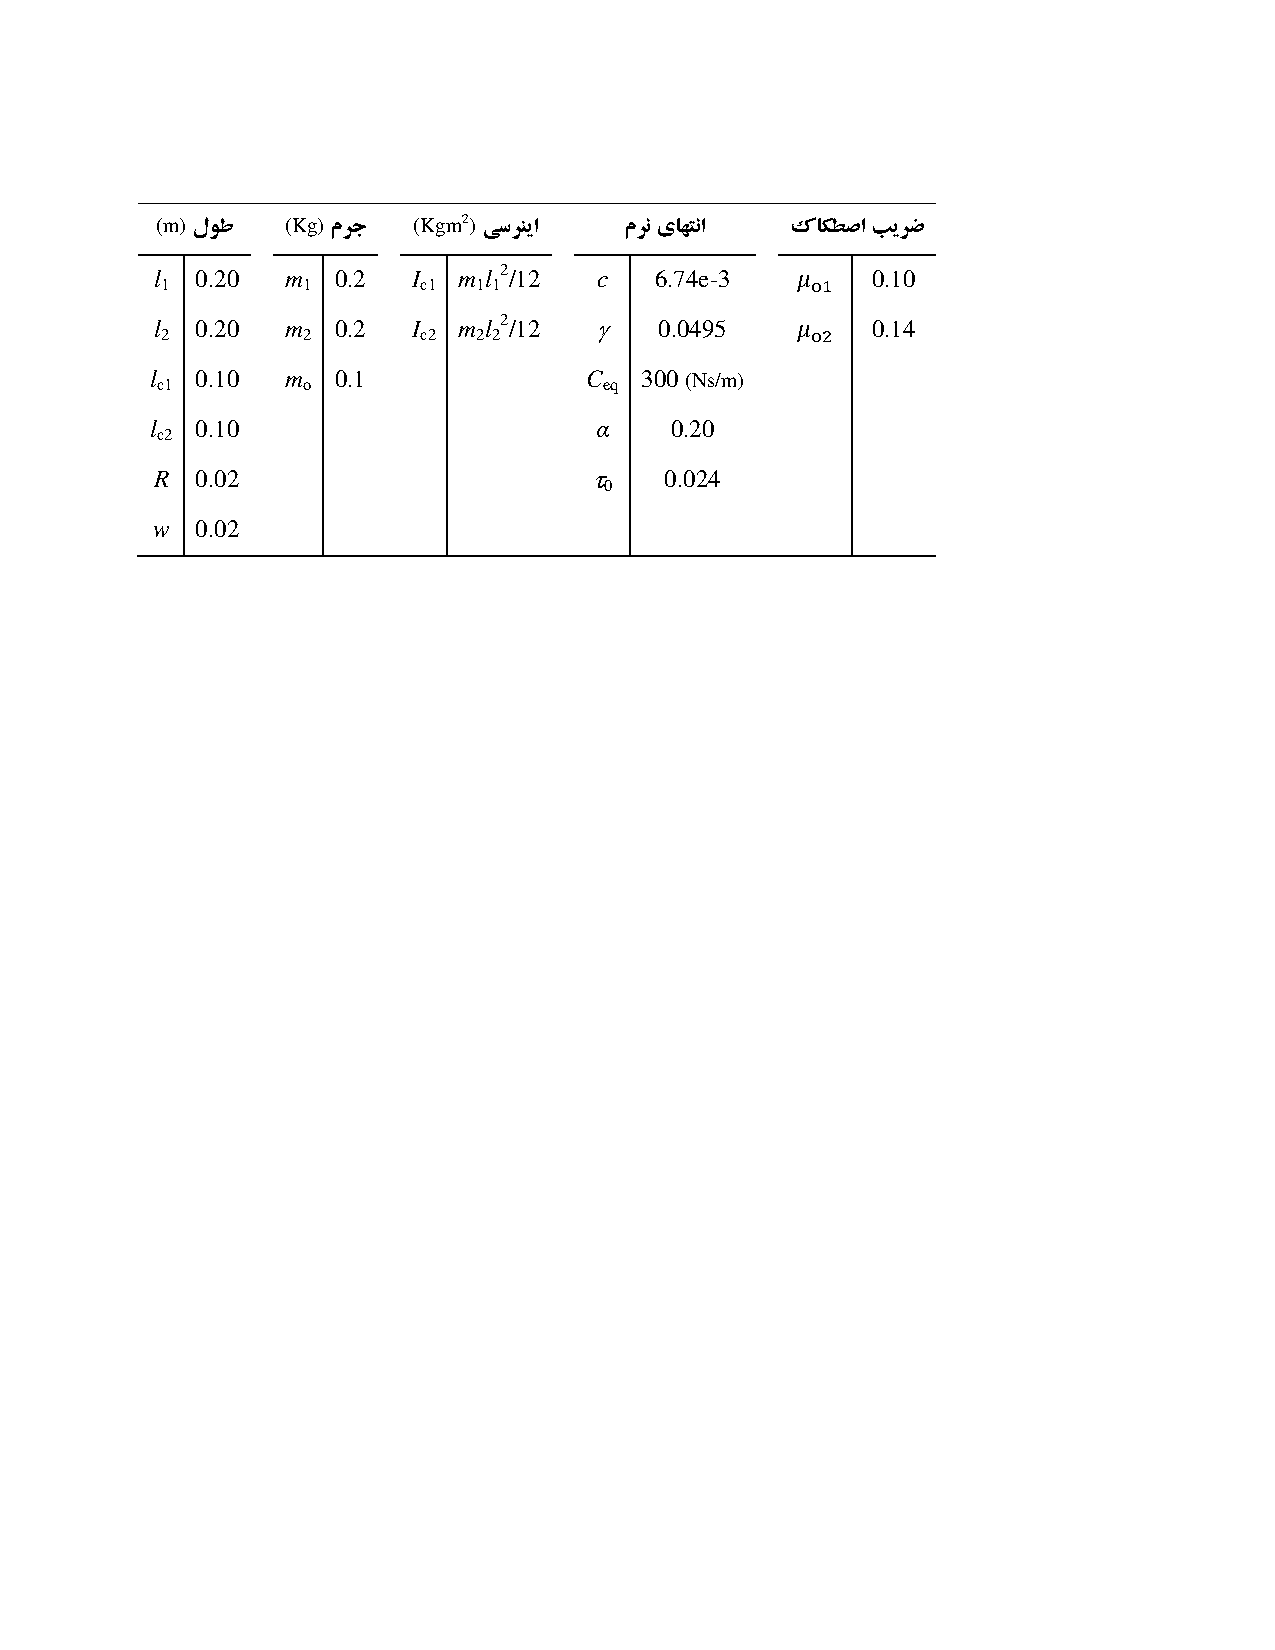
\includegraphics[scale=0.9]{Figures/SampleTable1.pdf} 
\end{tabular}
\vspace{-\baselineskip}
\label{Tbl:SampleTable1_2}
\end{table}

\begin{table}[!htb]
\caption{مقايسه‌ی روش‌هاي برداشت انرژي مبتني بر لرزش‌هاي مکانيکی}
\centering
\begin{tabular}{@{}|p{.15\textwidth}|p{.25\textwidth}|p{.25\textwidth}|p{.25\textwidth}|@{}}
\hline
روش
& 
چگالی انرژی
& 
ابعاد
& 
عیب اصلی
\\ \hline \hline
پیزوالکتریک
& 
$\mathrm{mJ/cm^3}$ 35/4
& 
بزرگ
& 
ولتاژ خروجی کم
\\ \hline
الکترومغناطیس
& 
$\mathrm{mJ/cm^3}$ 24/8
& 
بزرگ
& 
ولتاژ خروجی بسیار کم
\\ \hline
الکترواستاتیک
& 
$\mathrm{mJ/cm^3}$ 4
& 
فشرده در تراشه‌ها
& 
نیاز به منبع شارژ اولیه
\\ \hline
\end{tabular}
\label{Tbl:SampleTable2_2}
\vspace{-\baselineskip}
\end{table}

نمونه‌ای از یک رابطه به‌صورت
\begin{equation}
p\left( r \right) = {C_k}\frac{N}{{\pi {a^2}}}{\left[{1 - {{\left( {\frac{r}{a}} \right)}^k}} \right]^{\frac{1}{k}}},
\label{Eq:Pressure_2}
\end{equation}
است. در رابطه
\ref{Eq:Pressure_2}،
$N$
نیروی عمودی است. نمونه‌ای از استفاده از روابط متوالی به‌صورت
\begin{equation}
\sum \limits_{i = 1}^{k + 1} {E_s}\left( i \right) - T \sum \limits_{i = 1}^k {P_s}\left( i \right) \le B_s^{max},\quad k = 1, \ldots ,N - 1,
\label{Eq:batterysource_2}
\end{equation}\vspace{-\baselineskip}
\begin{equation}
\sum \limits_{i = 1}^{k + 1} {E_r}\left( i \right) - T \sum \limits_{i = 1}^k {P_r}\left( i \right) \le B_r^{max},\quad k = 1, \ldots ,N - 1,
\label{Eq:batteryrellay_2}
\end{equation}
است. نمونه‌ای از یک قضیه و تبصره نیز در ادامه آورده شده است.
\begin{theorem}
اگر ظرفیت باتری‌ها به اندازه کافی بزرگ باشد، جواب بهینه‌ی 
$P_s^*(i)$
و
$P_r^*(i)$
وجود دارد به نحوی که تابع هدف را بیشینه می‌کند و در رابطه‌ی زیر صدق می‌کند:
\begin{equation}
C\left( {{{\left| {{h_{sr}}\left( i \right)} \right|}^2}{P_s}^*\left( i \right)} \right) \ge C\left( {{{\left| {{h_{sd}}\left( i \right)} \right|}^2}{P_s}^*\left( i \right)} \right) + C\left( {{{\left| {{h_{rd}}\left( {i + 1} \right)} \right|}^2}P_r^*\left( {i} \right)} \right).
\label{Eq:theorem1_2}
\end{equation}

\begin{proof}
بار دیگر فرم تابع هدف را در نظر می‌گیریم. لازم به ذکر است اینجا تابع هدف یک تابع دومتغیره است.
\begin{equation}
{R({\mathbf{P}_s},{\mathbf{P}_r}) = {\frac{1}{2}\sum\limits_{i = 1}^N {\min } \left\{ {C\left( {{{\left| {{h_{sr}}\left( i \right)} \right|}^2}{P_s}\left( i \right)} \right),} C\left( {{{\left| {{h_{sd}}\left( i \right)} \right|}^2}{P_s}\left( i \right)} \right) \right\} }}.
\end{equation}
حال بلوک
$i$ام
را در نظر می‌گیریم. اگر رابطه‌ی
\ref{Eq:theorem1_2}
برای
$i$
برقرار نباشد، به عبارت دیگر اگر داشته باشیم،
\begin{equation}
C\left( {{{\left| {{h_{sr}}\left( i \right)} \right|}^2}{P_s}^*\left( i \right)} \right) < C\left( {{{\left| {{h_{sd}}\left( i \right)} \right|}^2}{P_s}^*\left( i \right)} \right) + C\left( {{{\left| {{h_{rd}}\left( {i + 1} \right)} \right|}^2}P_r^*\left( {i + 1} \right)} \right),
\label{Eq:theorem1(2)_2}
\end{equation}
بنابراین
\begin{equation}
C\left( {{{\left| {{h_{sr}}\left( i \right)} \right|}^2}{P_s}^*\left( i \right)} \right)+ C\left( {{{\left| {{h_{sd}}\left( i \right)} \right|}^2}{P_s}^*\left( i \right)} \right) =C\left( {{{\left| {{h_{sr}}\left( i \right)} \right|}^2}{P_s}^*\left( i \right)} \right).
\end{equation}
پس در تابع هدف مسئله، مقدار بهینه‌ی مسئله برابر عبارت سمت چپ رابطه‌ی
\ref{Eq:theorem1(2)_2}
شده است و آرگومان دوم و  هم‌چنین مقدار
$P_r^*(i)$
هیچ نقشی در مقدار بهینه ندارد. بنابراین می‌توانیم 
$P_r^*(i)$
را آنقدر کاهش دهیم تا در رابطه‌ی
\ref{Eq:theorem1(2)_2}
تساوی برقرار شود بدون آنکه مقدار بهینه‌ی مسئله تغییر کند.
\end{proof}
\label{theorem1_2}
\end{theorem}

\begin{remark}
از قضیه‌ی
\ref{theorem1_2}
نتیجه می‌گیریم که جواب بهینه‌ی مسئله‌ی
\lr{P}
در حالت کلی یکتا نیست. به طور مثال وقتی مقدار انرژی برداشت‌شده در رله خیلی بیشتر از این انرژی در منبع باشد مسئله می‌تواند جواب‌های زیادی داشته باشد. بنابراین همواره می‌توان برای صرفه‌جویی در مصرف انرژی، بدون کاهش مقدار نرخ گذردهی سیستم، کمترین مقدار توان را برای رله انتخاب کرد. بنابراین با توجه به رابطه
\begin{equation}
C\left( {{{\left| {{h_{sr}}\left( i \right)} \right|}^2}{P_s}^*\left( i \right)} \right) 
\ge C\left( {{{\left| {{h_{sd}}\left( i \right)} \right|}^2}{P_s}^*\left( i \right)} \right) + C\left( {{{\left| {{h_{rd}}\left( {i} \right)} \right|}^2}P_r^*\left( {i} \right)} \right),
\label{Eq:remark1_2}
\end{equation}
و با  استفاده از رابطه
\ref{Eq:remark1_2}
خواهیم داشت،
\begin{equation}
{R_r}(i) = \min \left\{ {C\left( {{{\left| {{h_{rd}}(i)} \right|}^2}{P_r}(i)} \right),C\left( {{{\left| {{h_{sr}}(i)} \right|}^2}{P_s}(i)} \right)} \right\}.
\end{equation}

بنابراین می‌توان با انتخاب کمترین توان و نرخ برای رله از مصرف بی‌رویه‌ی انرژی جلوگیری کرد. فرض بزرگ بودن ظرفیت باتری‌ به این دلیل است که اگر ظرفیت باتری محدود باشد برای کاهش
$P_r^*(i)$
با محدودیت مواجه هستیم. چون در صورت کاهش بی از حد توان رله ممکن است از ناحیه‌ی شدنی مسئله خارج شویم. به هر حال برای هر دو حالت ظرفیت نامحدود و محدود باتری جواب مسئله یکتا نیست و همواره می‌توان با کاهش توان رله مصرف انرژی را کاهش داد.
\end{remark}

\section{پیش‌گفتار}
در این قالب سعی شده است که از تمامی بخش‌های موجود در پایان‌نامه‌ها نمونه‌ای آورده شود. در این قالب سعی شده است که از تمامی بخش‌های موجود در پایان‌نامه‌ها نمونه‌ای آورده شود. در این قالب سعی شده است که از تمامی بخش‌های موجود در پایان‌نامه‌ها نمونه‌ای آورده شود. در این قالب سعی شده است که از تمامی بخش‌های موجود در پایان‌نامه‌ها نمونه‌ای آورده شود. در این قالب سعی شده است که از تمامی بخش‌های موجود در پایان‌نامه‌ها نمونه‌ای آورده شود. در این قالب سعی شده است که از تمامی بخش‌های موجود در پایان‌نامه‌ها نمونه‌ای آورده شود. در این قالب سعی شده است که از تمامی بخش‌های موجود در پایان‌نامه‌ها نمونه‌ای آورده شود. در این قالب سعی شده است که از تمامی بخش‌های موجود در پایان‌نامه‌ها نمونه‌ای آورده شود. در این قالب سعی شده است که از تمامی بخش‌های موجود در پایان‌نامه‌ها نمونه‌ای آورده شود. در این قالب سعی شده است که از تمامی بخش‌های موجود در پایان‌نامه‌ها نمونه‌ای آورده شود. در این قالب سعی شده است که از تمامی بخش‌های موجود در پایان‌نامه‌ها نمونه‌ای آورده شود. در این قالب سعی شده است که از تمامی بخش‌های موجود در پایان‌نامه‌ها نمونه‌ای آورده شود. در این قالب سعی شده است که از تمامی بخش‌های موجود در پایان‌نامه‌ها نمونه‌ای آورده شود. در این قالب سعی شده است که از تمامی بخش‌های موجود در پایان‌نامه‌ها نمونه‌ای آورده شود.
\section{بخش اول}
نمونه‌ای از یک عبارت انگلیسی در متن به‌صورت
\lr{English Sentence}
است. نمونه‌ای از یک عبارت ریاضی در متن نیز به‌صورت
$x^2 + y^2$
است. ارجاع به مراجع انگلیسی
\cite{Fakhari2015a,Lewis2003}.
ارجاع به مراجع فارسی
\cite{Fakhari2015b,HadianThesis2008}.
این نمونه‌ای از یک زیرنویس انگلیسی%
\LTRfootnote{English Footnote}
است. این نمونه‌ای از یک زیرنویس فارسی%
\RTLfootnote{زیرنویس فارسی}
است. در شکل
\ref{Fig:SampleFigure1_2}،
نمونه‌ای از یک شکل آورده شده است. 

\begin{figure}[!htb]
\centering
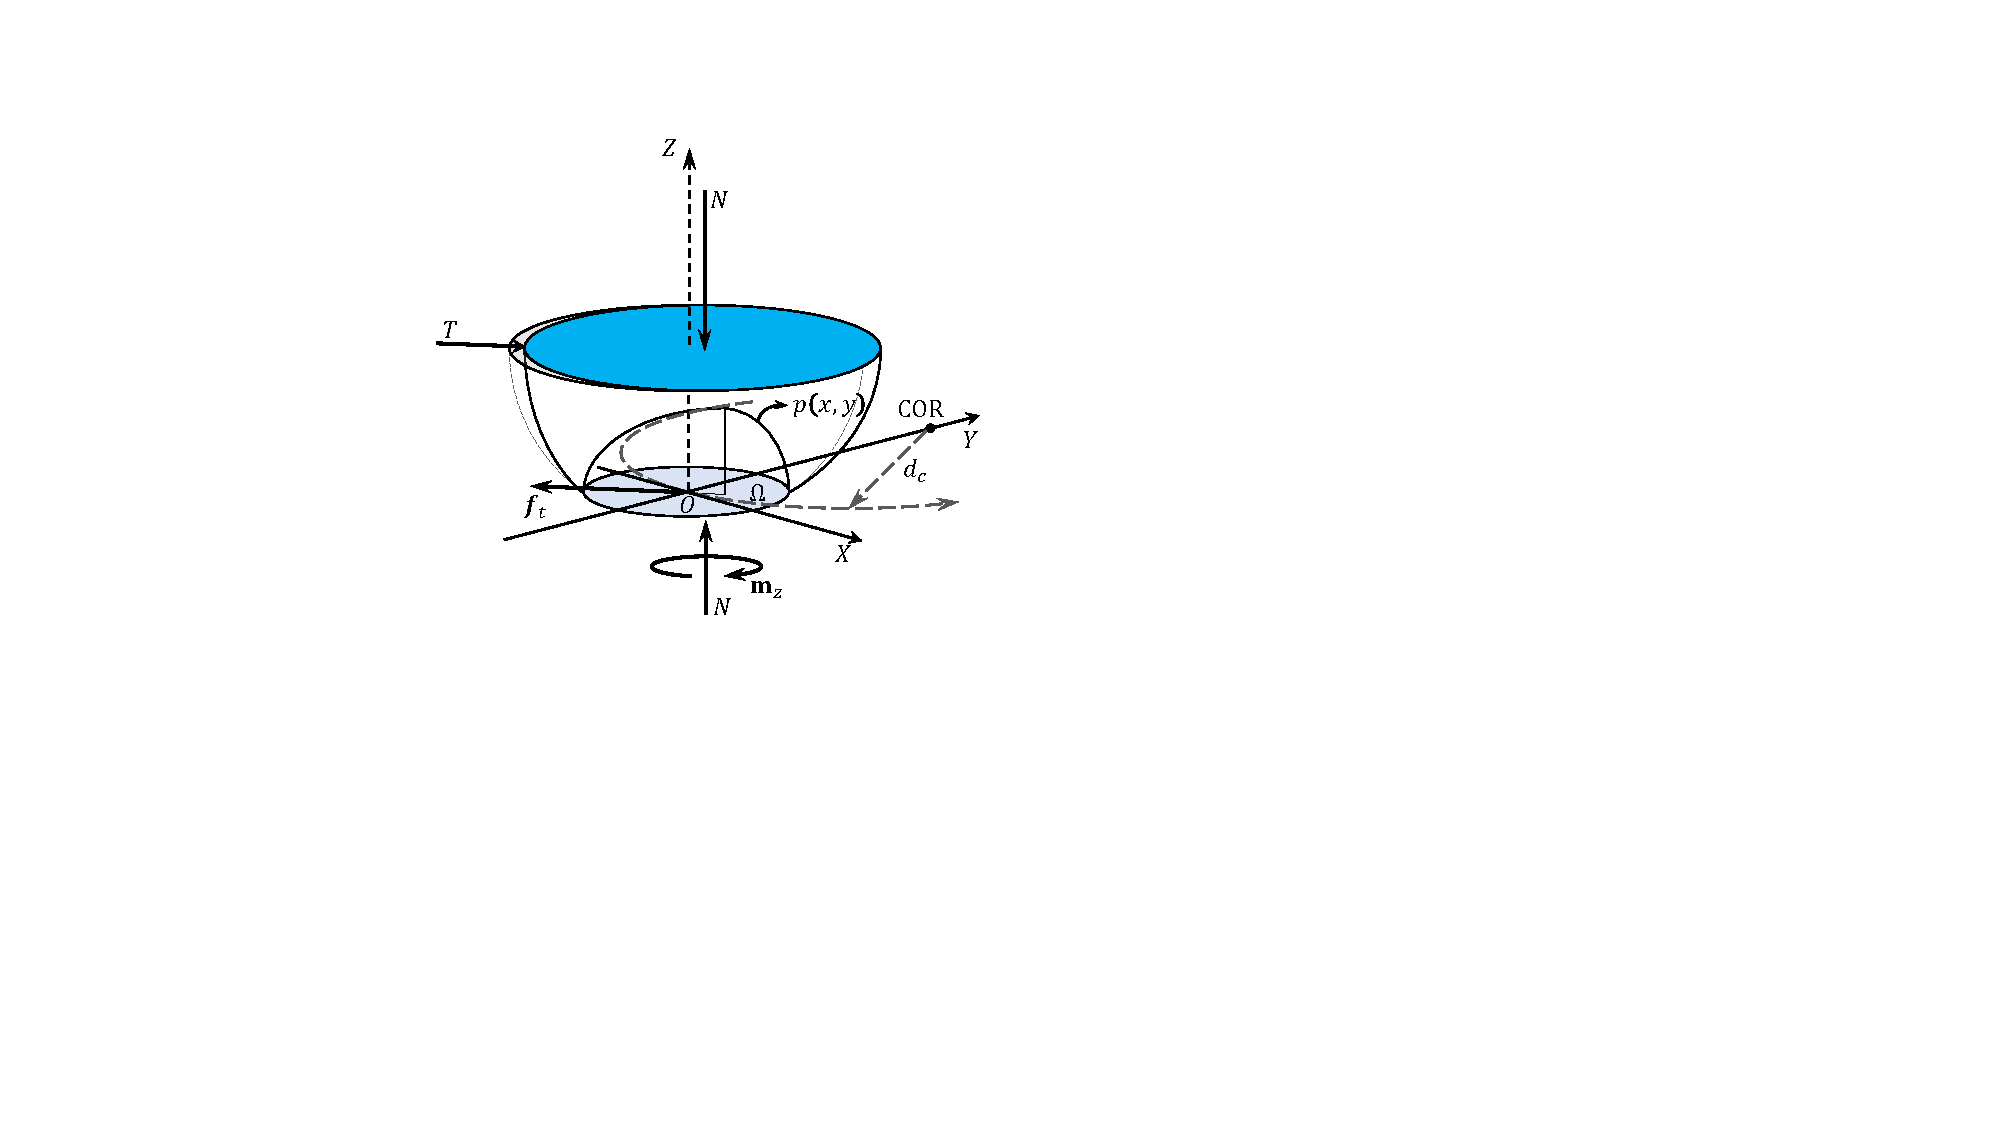
\includegraphics[scale=1]{Figures/SampleFigure.pdf}
\caption{شکل نمونه}
\label{Fig:SampleFigure1_2}
\end{figure}

نمونه‌ای از قرار دادن دو شکل در کنار یکدیگر در شکل
\ref{Fig:SampleFigure2_2}
آورده شده است.

\begin{figure}[!htb]
\centering
\subfloat[زیرنویس شکل اول]{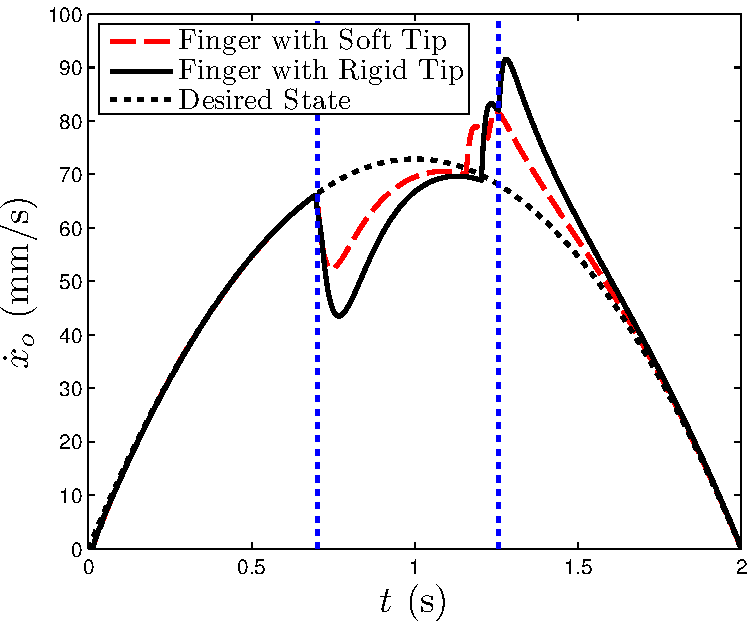
\includegraphics[scale=0.56]{Figures/FigureA.pdf}}
\quad
\subfloat[زیرنویس شکل دوم]{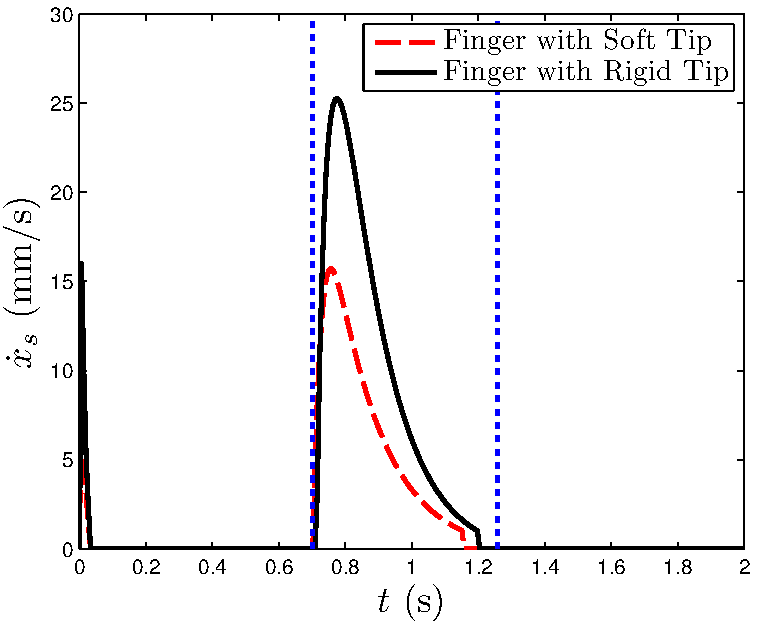
\includegraphics[scale=0.56]{Figures/FigureB.pdf}}
\caption{
قرار دادن دو شکل در کنار یکدیگر، الف) شکل نمونه اول،
ب) شکل نمونه دوم
}
\label{Fig:SampleFigure2_2}
\end{figure}





آیتم‌های مختلف به‌صورت زیر آورده می‌شود:
\begin{itemize}[label=-]
\item
مورد اول
\item
مورد دوم
\item
مورد سوم
\end{itemize}

نمونه‌ای از آیتم‌های شماره‌دار نیز در ادامه آورده شده است. به طور کلی معماری برداشت انرژی به دو دسته‌ی کلی تقسیم می‌شود:
\begin{enumerate}[label=\arabic*)]
\item
برداشت-استفاده:

در این حالت سیستم بلافاصله انرژی برداشت‌شده را مصرف می‌کند. واضح است اگر انرژی کافی در محیط وجود نداشته باشد دستگاه از کار می‌افتد. این نوع سیستم‌ها بیشتر در فشار دادن کلید‌ها، پدال‌ها و دستگاه‌های ردیابی برای انسان‌ها استفاده می‌شود. به طور مثال در پاشنه‌ی کفش دونده‌ای مواد پیزوالکتریک کار گذاشته می‌شود و با فشار پا بر روی کفش و فشرده شدن پیزوالکتریک داخل کفش، انرژی الکتریکی برای ارسال سیگنال 
\lr{RF}
و در نتیجه ردیابی دونده تامین می‌شود. 
\item
برداشت-ذخیره-استفاده:

در این روش سیستم برای ذخیره‌ی انرژی برداشت‌شده به باتری مجهز شده است. این روش برای زمانی‌که انرژی زیادی در محیط وجود داشته باشد و برای منابعی مانند انرژی خورشیدی  کاربرد دارد. روش‌های زیادی برای تبدیل انرژی خورشیدی به انرژی الکتریکی از جمله سلول‌های خورشیدی وجود دارد. در این حالت چگونگی ذخیره‌ی انرژی و بهینه‌سازی مصرف انرژی مطرح می‌شود.
\end{enumerate}




\subsection{زیربخش اول}
نوشته نمونه نوشته نمونه نوشته نمونه نوشته نمونه نوشته نمونه نوشته نمونه نوشته نمونه نوشته نمونه نوشته نمونه نوشته نمونه نوشته نمونه نوشته نمونه نوشته نمونه نوشته نمونه نوشته نمونه نوشته نمونه نوشته نمونه نوشته نمونه نوشته نمونه نوشته نمونه نوشته نمونه نوشته نمونه. در جدول
\ref{Tbl:SampleTable1_2}،
نمونه‌ای از یک جدول واردشده در لاتک و در جدول
\ref{Tbl:SampleTable2_2}،
نمونه‌ای از یک جدول نوشته‌شده در لاتک آورده شده است.

\begin{table}[!htb]
\caption{پارامترهای شبیه‌سازی}
\centering
\begin{tabular}{c}
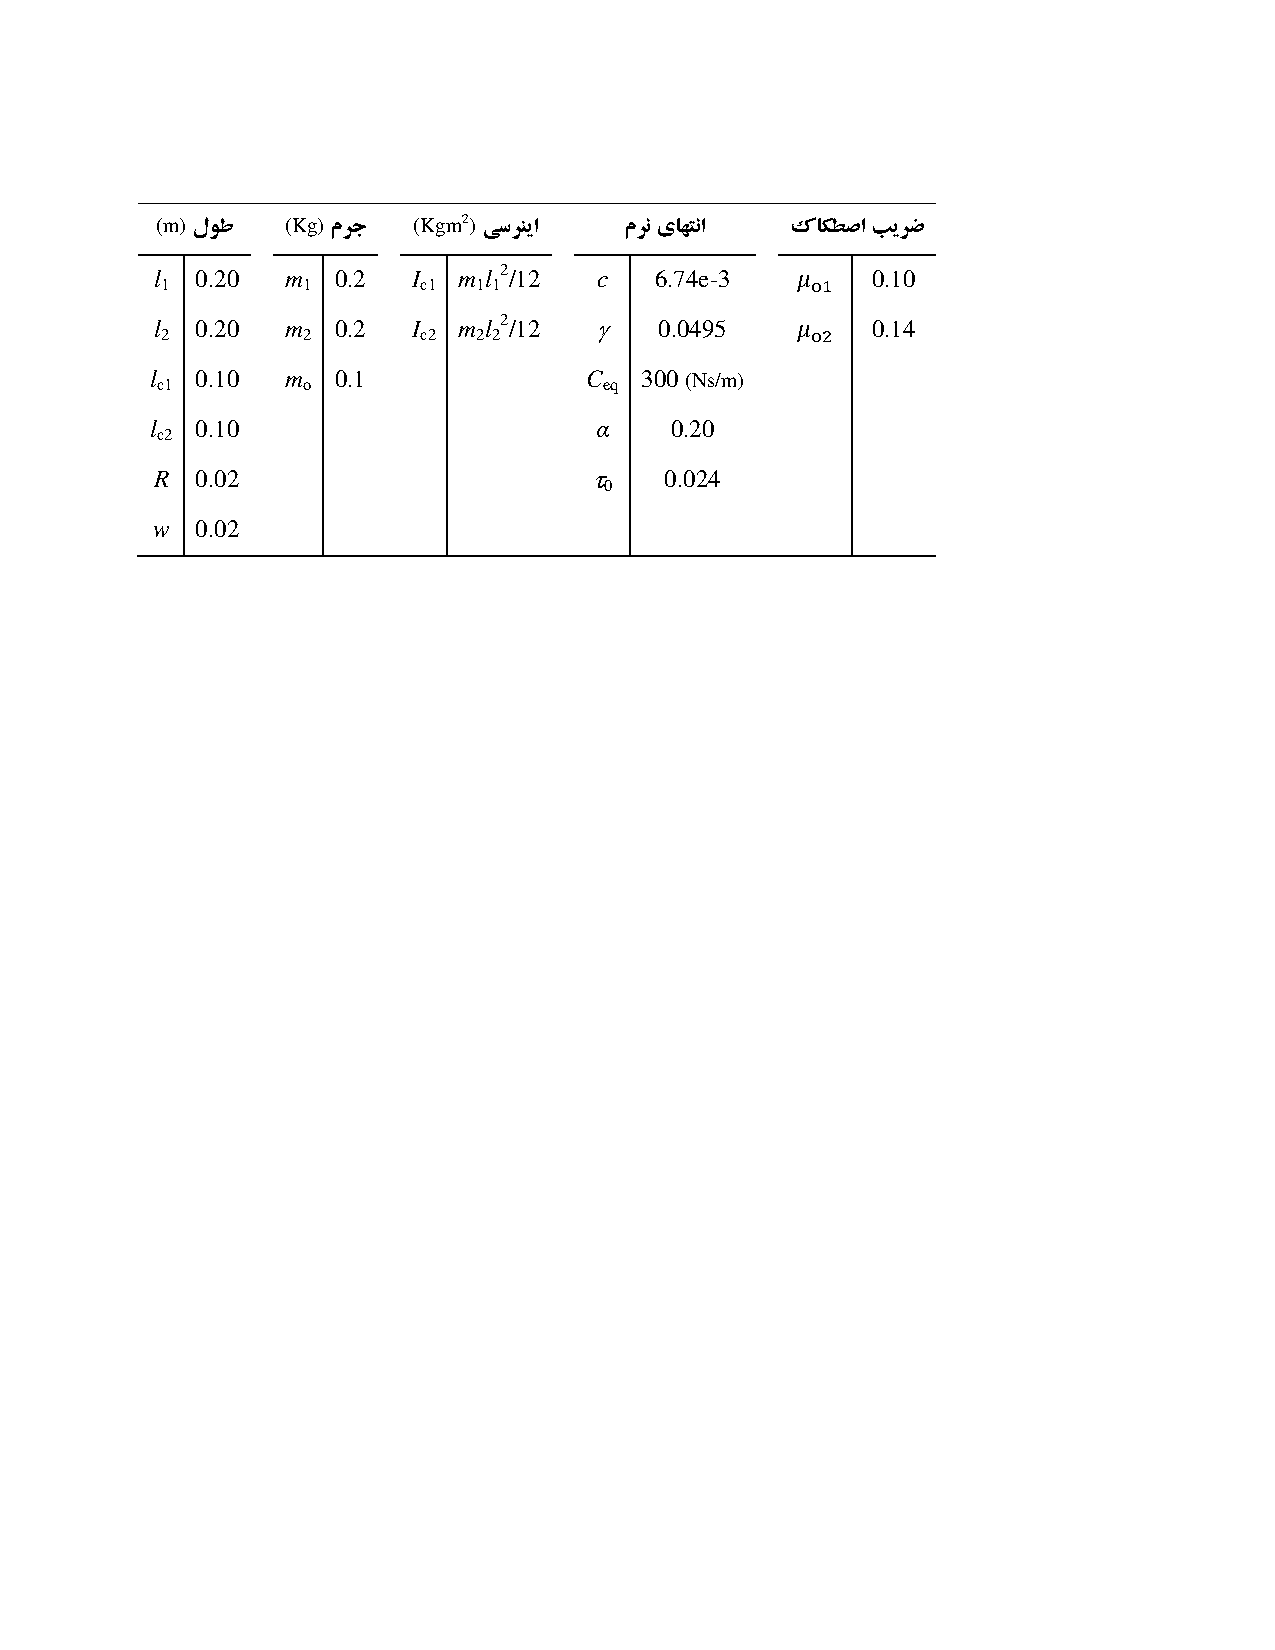
\includegraphics[scale=0.9]{Figures/SampleTable1.pdf} 
\end{tabular}
\vspace{-\baselineskip}
\label{Tbl:SampleTable1_2}
\end{table}

\begin{table}[!htb]
\caption{مقايسه‌ی روش‌هاي برداشت انرژي مبتني بر لرزش‌هاي مکانيکی}
\centering
\begin{tabular}{@{}|p{.15\textwidth}|p{.25\textwidth}|p{.25\textwidth}|p{.25\textwidth}|@{}}
\hline
روش
& 
چگالی انرژی
& 
ابعاد
& 
عیب اصلی
\\ \hline \hline
پیزوالکتریک
& 
$\mathrm{mJ/cm^3}$ 35/4
& 
بزرگ
& 
ولتاژ خروجی کم
\\ \hline
الکترومغناطیس
& 
$\mathrm{mJ/cm^3}$ 24/8
& 
بزرگ
& 
ولتاژ خروجی بسیار کم
\\ \hline
الکترواستاتیک
& 
$\mathrm{mJ/cm^3}$ 4
& 
فشرده در تراشه‌ها
& 
نیاز به منبع شارژ اولیه
\\ \hline
\end{tabular}
\label{Tbl:SampleTable2_2}
\vspace{-\baselineskip}
\end{table}

نمونه‌ای از یک رابطه به‌صورت
\begin{equation}
p\left( r \right) = {C_k}\frac{N}{{\pi {a^2}}}{\left[{1 - {{\left( {\frac{r}{a}} \right)}^k}} \right]^{\frac{1}{k}}},
\label{Eq:Pressure_2}
\end{equation}
است. در رابطه
\ref{Eq:Pressure_2}،
$N$
نیروی عمودی است. نمونه‌ای از استفاده از روابط متوالی به‌صورت
\begin{equation}
\sum \limits_{i = 1}^{k + 1} {E_s}\left( i \right) - T \sum \limits_{i = 1}^k {P_s}\left( i \right) \le B_s^{max},\quad k = 1, \ldots ,N - 1,
\label{Eq:batterysource_2}
\end{equation}\vspace{-\baselineskip}
\begin{equation}
\sum \limits_{i = 1}^{k + 1} {E_r}\left( i \right) - T \sum \limits_{i = 1}^k {P_r}\left( i \right) \le B_r^{max},\quad k = 1, \ldots ,N - 1,
\label{Eq:batteryrellay_2}
\end{equation}
است. نمونه‌ای از یک قضیه و تبصره نیز در ادامه آورده شده است.
\begin{theorem}
اگر ظرفیت باتری‌ها به اندازه کافی بزرگ باشد، جواب بهینه‌ی 
$P_s^*(i)$
و
$P_r^*(i)$
وجود دارد به نحوی که تابع هدف را بیشینه می‌کند و در رابطه‌ی زیر صدق می‌کند:
\begin{equation}
C\left( {{{\left| {{h_{sr}}\left( i \right)} \right|}^2}{P_s}^*\left( i \right)} \right) \ge C\left( {{{\left| {{h_{sd}}\left( i \right)} \right|}^2}{P_s}^*\left( i \right)} \right) + C\left( {{{\left| {{h_{rd}}\left( {i + 1} \right)} \right|}^2}P_r^*\left( {i} \right)} \right).
\label{Eq:theorem1_2}
\end{equation}

\begin{proof}
بار دیگر فرم تابع هدف را در نظر می‌گیریم. لازم به ذکر است اینجا تابع هدف یک تابع دومتغیره است.
\begin{equation}
{R({\mathbf{P}_s},{\mathbf{P}_r}) = {\frac{1}{2}\sum\limits_{i = 1}^N {\min } \left\{ {C\left( {{{\left| {{h_{sr}}\left( i \right)} \right|}^2}{P_s}\left( i \right)} \right),} C\left( {{{\left| {{h_{sd}}\left( i \right)} \right|}^2}{P_s}\left( i \right)} \right) \right\} }}.
\end{equation}
حال بلوک
$i$ام
را در نظر می‌گیریم. اگر رابطه‌ی
\ref{Eq:theorem1_2}
برای
$i$
برقرار نباشد، به عبارت دیگر اگر داشته باشیم،
\begin{equation}
C\left( {{{\left| {{h_{sr}}\left( i \right)} \right|}^2}{P_s}^*\left( i \right)} \right) < C\left( {{{\left| {{h_{sd}}\left( i \right)} \right|}^2}{P_s}^*\left( i \right)} \right) + C\left( {{{\left| {{h_{rd}}\left( {i + 1} \right)} \right|}^2}P_r^*\left( {i + 1} \right)} \right),
\label{Eq:theorem1(2)_2}
\end{equation}
بنابراین
\begin{equation}
C\left( {{{\left| {{h_{sr}}\left( i \right)} \right|}^2}{P_s}^*\left( i \right)} \right)+ C\left( {{{\left| {{h_{sd}}\left( i \right)} \right|}^2}{P_s}^*\left( i \right)} \right) =C\left( {{{\left| {{h_{sr}}\left( i \right)} \right|}^2}{P_s}^*\left( i \right)} \right).
\end{equation}
پس در تابع هدف مسئله، مقدار بهینه‌ی مسئله برابر عبارت سمت چپ رابطه‌ی
\ref{Eq:theorem1(2)_2}
شده است و آرگومان دوم و  هم‌چنین مقدار
$P_r^*(i)$
هیچ نقشی در مقدار بهینه ندارد. بنابراین می‌توانیم 
$P_r^*(i)$
را آنقدر کاهش دهیم تا در رابطه‌ی
\ref{Eq:theorem1(2)_2}
تساوی برقرار شود بدون آنکه مقدار بهینه‌ی مسئله تغییر کند.
\end{proof}
\label{theorem1_2}
\end{theorem}

\begin{remark}
از قضیه‌ی
\ref{theorem1_2}
نتیجه می‌گیریم که جواب بهینه‌ی مسئله‌ی
\lr{P}
در حالت کلی یکتا نیست. به طور مثال وقتی مقدار انرژی برداشت‌شده در رله خیلی بیشتر از این انرژی در منبع باشد مسئله می‌تواند جواب‌های زیادی داشته باشد. بنابراین همواره می‌توان برای صرفه‌جویی در مصرف انرژی، بدون کاهش مقدار نرخ گذردهی سیستم، کمترین مقدار توان را برای رله انتخاب کرد. بنابراین با توجه به رابطه
\begin{equation}
C\left( {{{\left| {{h_{sr}}\left( i \right)} \right|}^2}{P_s}^*\left( i \right)} \right) 
\ge C\left( {{{\left| {{h_{sd}}\left( i \right)} \right|}^2}{P_s}^*\left( i \right)} \right) + C\left( {{{\left| {{h_{rd}}\left( {i} \right)} \right|}^2}P_r^*\left( {i} \right)} \right),
\label{Eq:remark1_2}
\end{equation}
و با  استفاده از رابطه
\ref{Eq:remark1_2}
خواهیم داشت،
\begin{equation}
{R_r}(i) = \min \left\{ {C\left( {{{\left| {{h_{rd}}(i)} \right|}^2}{P_r}(i)} \right),C\left( {{{\left| {{h_{sr}}(i)} \right|}^2}{P_s}(i)} \right)} \right\}.
\end{equation}

بنابراین می‌توان با انتخاب کمترین توان و نرخ برای رله از مصرف بی‌رویه‌ی انرژی جلوگیری کرد. فرض بزرگ بودن ظرفیت باتری‌ به این دلیل است که اگر ظرفیت باتری محدود باشد برای کاهش
$P_r^*(i)$
با محدودیت مواجه هستیم. چون در صورت کاهش بی از حد توان رله ممکن است از ناحیه‌ی شدنی مسئله خارج شویم. به هر حال برای هر دو حالت ظرفیت نامحدود و محدود باتری جواب مسئله یکتا نیست و همواره می‌توان با کاهش توان رله مصرف انرژی را کاهش داد.
\end{remark}


\section{پیش‌گفتار}
در این قالب سعی شده است که از تمامی بخش‌های موجود در پایان‌نامه‌ها نمونه‌ای آورده شود. در این قالب سعی شده است که از تمامی بخش‌های موجود در پایان‌نامه‌ها نمونه‌ای آورده شود. در این قالب سعی شده است که از تمامی بخش‌های موجود در پایان‌نامه‌ها نمونه‌ای آورده شود. در این قالب سعی شده است که از تمامی بخش‌های موجود در پایان‌نامه‌ها نمونه‌ای آورده شود. در این قالب سعی شده است که از تمامی بخش‌های موجود در پایان‌نامه‌ها نمونه‌ای آورده شود. در این قالب سعی شده است که از تمامی بخش‌های موجود در پایان‌نامه‌ها نمونه‌ای آورده شود. در این قالب سعی شده است که از تمامی بخش‌های موجود در پایان‌نامه‌ها نمونه‌ای آورده شود. در این قالب سعی شده است که از تمامی بخش‌های موجود در پایان‌نامه‌ها نمونه‌ای آورده شود. در این قالب سعی شده است که از تمامی بخش‌های موجود در پایان‌نامه‌ها نمونه‌ای آورده شود. در این قالب سعی شده است که از تمامی بخش‌های موجود در پایان‌نامه‌ها نمونه‌ای آورده شود. در این قالب سعی شده است که از تمامی بخش‌های موجود در پایان‌نامه‌ها نمونه‌ای آورده شود. در این قالب سعی شده است که از تمامی بخش‌های موجود در پایان‌نامه‌ها نمونه‌ای آورده شود. در این قالب سعی شده است که از تمامی بخش‌های موجود در پایان‌نامه‌ها نمونه‌ای آورده شود. در این قالب سعی شده است که از تمامی بخش‌های موجود در پایان‌نامه‌ها نمونه‌ای آورده شود.
\section{بخش اول}
نمونه‌ای از یک عبارت انگلیسی در متن به‌صورت
\lr{English Sentence}
است. نمونه‌ای از یک عبارت ریاضی در متن نیز به‌صورت
$x^2 + y^2$
است. ارجاع به مراجع انگلیسی
\cite{Fakhari2015a,Lewis2003}.
ارجاع به مراجع فارسی
\cite{Fakhari2015b,HadianThesis2008}.
این نمونه‌ای از یک زیرنویس انگلیسی%
\LTRfootnote{English Footnote}
است. این نمونه‌ای از یک زیرنویس فارسی%
\RTLfootnote{زیرنویس فارسی}
است. در شکل
\ref{Fig:SampleFigure1_2}،
نمونه‌ای از یک شکل آورده شده است. 

\begin{figure}[!htb]
\centering
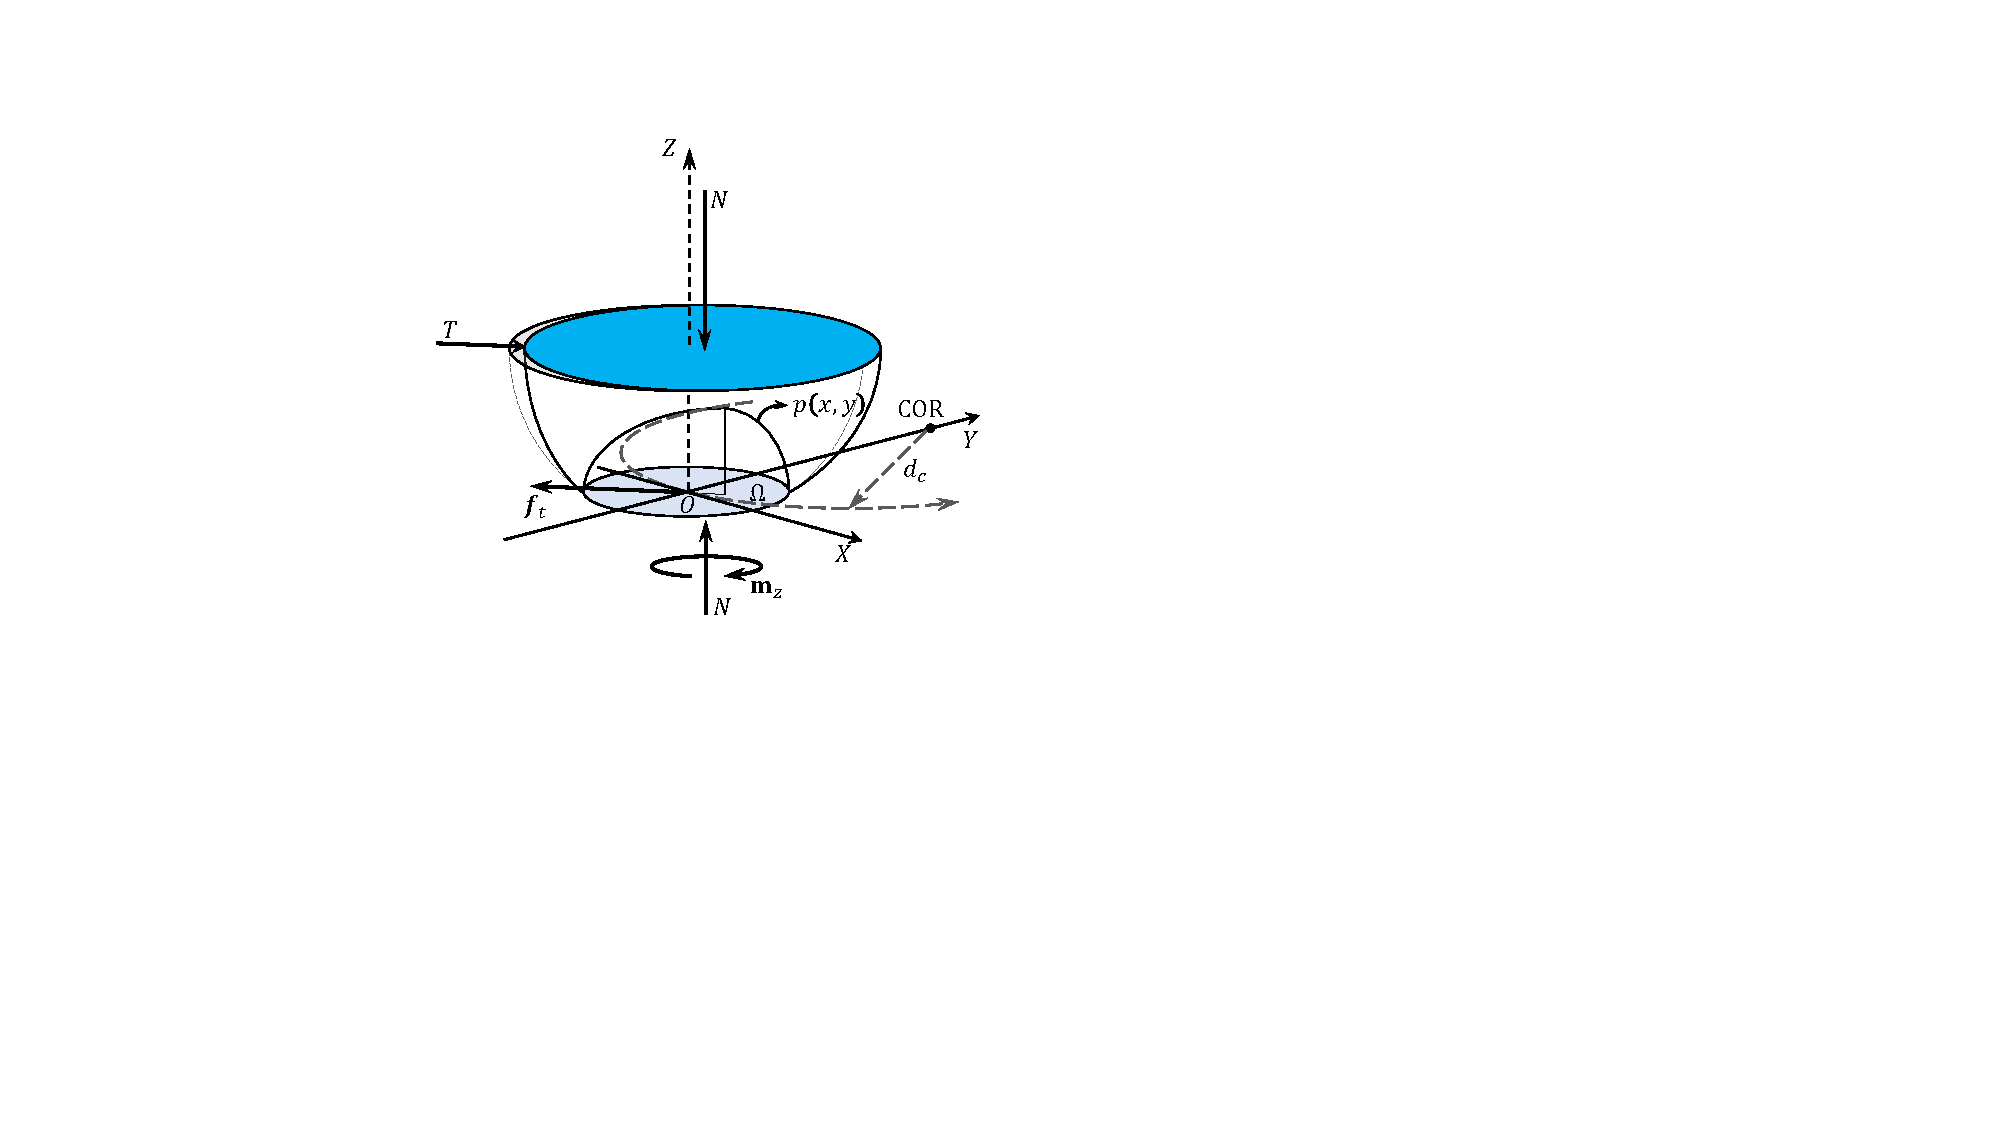
\includegraphics[scale=1]{Figures/SampleFigure.pdf}
\caption{شکل نمونه}
\label{Fig:SampleFigure1_2}
\end{figure}

نمونه‌ای از قرار دادن دو شکل در کنار یکدیگر در شکل
\ref{Fig:SampleFigure2_2}
آورده شده است.

\begin{figure}[!htb]
\centering
\subfloat[زیرنویس شکل اول]{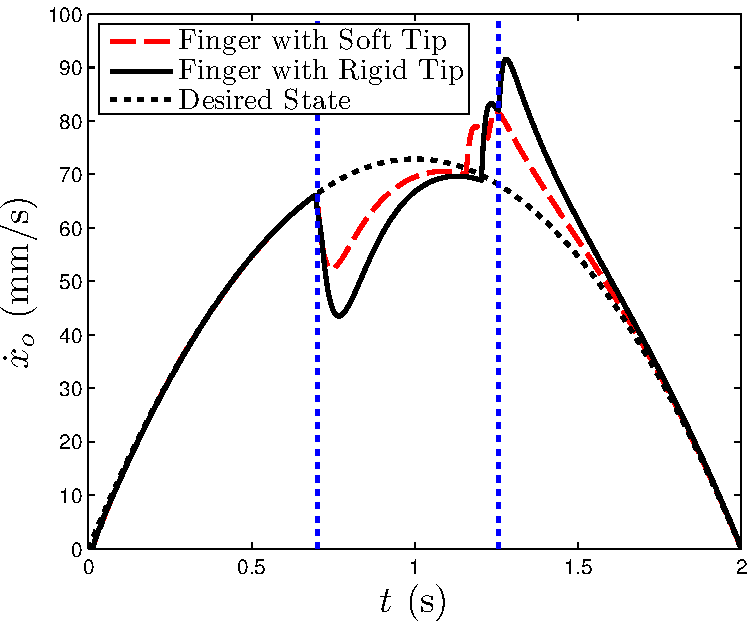
\includegraphics[scale=0.56]{Figures/FigureA.pdf}}
\quad
\subfloat[زیرنویس شکل دوم]{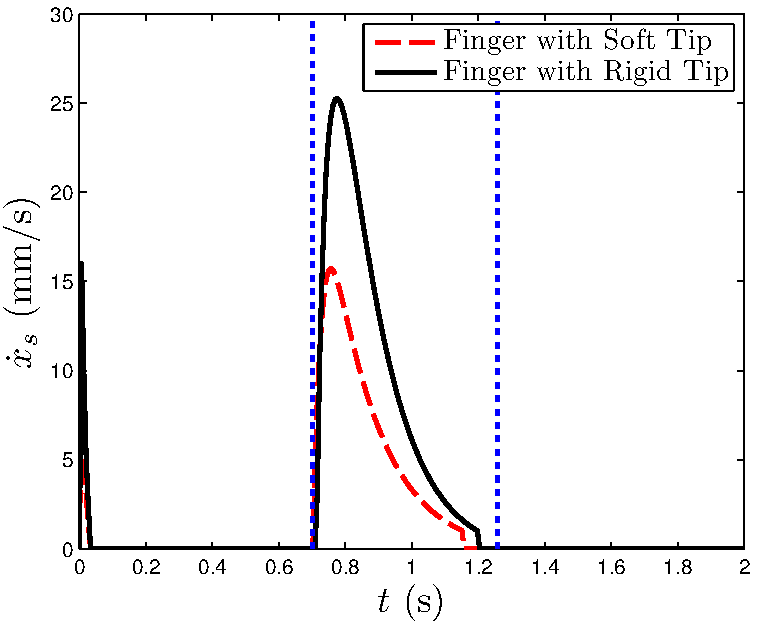
\includegraphics[scale=0.56]{Figures/FigureB.pdf}}
\caption{
قرار دادن دو شکل در کنار یکدیگر، الف) شکل نمونه اول،
ب) شکل نمونه دوم
}
\label{Fig:SampleFigure2_2}
\end{figure}





آیتم‌های مختلف به‌صورت زیر آورده می‌شود:
\begin{itemize}[label=-]
\item
مورد اول
\item
مورد دوم
\item
مورد سوم
\end{itemize}

نمونه‌ای از آیتم‌های شماره‌دار نیز در ادامه آورده شده است. به طور کلی معماری برداشت انرژی به دو دسته‌ی کلی تقسیم می‌شود:
\begin{enumerate}[label=\arabic*)]
\item
برداشت-استفاده:

در این حالت سیستم بلافاصله انرژی برداشت‌شده را مصرف می‌کند. واضح است اگر انرژی کافی در محیط وجود نداشته باشد دستگاه از کار می‌افتد. این نوع سیستم‌ها بیشتر در فشار دادن کلید‌ها، پدال‌ها و دستگاه‌های ردیابی برای انسان‌ها استفاده می‌شود. به طور مثال در پاشنه‌ی کفش دونده‌ای مواد پیزوالکتریک کار گذاشته می‌شود و با فشار پا بر روی کفش و فشرده شدن پیزوالکتریک داخل کفش، انرژی الکتریکی برای ارسال سیگنال 
\lr{RF}
و در نتیجه ردیابی دونده تامین می‌شود. 
\item
برداشت-ذخیره-استفاده:

در این روش سیستم برای ذخیره‌ی انرژی برداشت‌شده به باتری مجهز شده است. این روش برای زمانی‌که انرژی زیادی در محیط وجود داشته باشد و برای منابعی مانند انرژی خورشیدی  کاربرد دارد. روش‌های زیادی برای تبدیل انرژی خورشیدی به انرژی الکتریکی از جمله سلول‌های خورشیدی وجود دارد. در این حالت چگونگی ذخیره‌ی انرژی و بهینه‌سازی مصرف انرژی مطرح می‌شود.
\end{enumerate}




\subsection{زیربخش اول}
نوشته نمونه نوشته نمونه نوشته نمونه نوشته نمونه نوشته نمونه نوشته نمونه نوشته نمونه نوشته نمونه نوشته نمونه نوشته نمونه نوشته نمونه نوشته نمونه نوشته نمونه نوشته نمونه نوشته نمونه نوشته نمونه نوشته نمونه نوشته نمونه نوشته نمونه نوشته نمونه نوشته نمونه نوشته نمونه. در جدول
\ref{Tbl:SampleTable1_2}،
نمونه‌ای از یک جدول واردشده در لاتک و در جدول
\ref{Tbl:SampleTable2_2}،
نمونه‌ای از یک جدول نوشته‌شده در لاتک آورده شده است.

\begin{table}[!htb]
\caption{پارامترهای شبیه‌سازی}
\centering
\begin{tabular}{c}
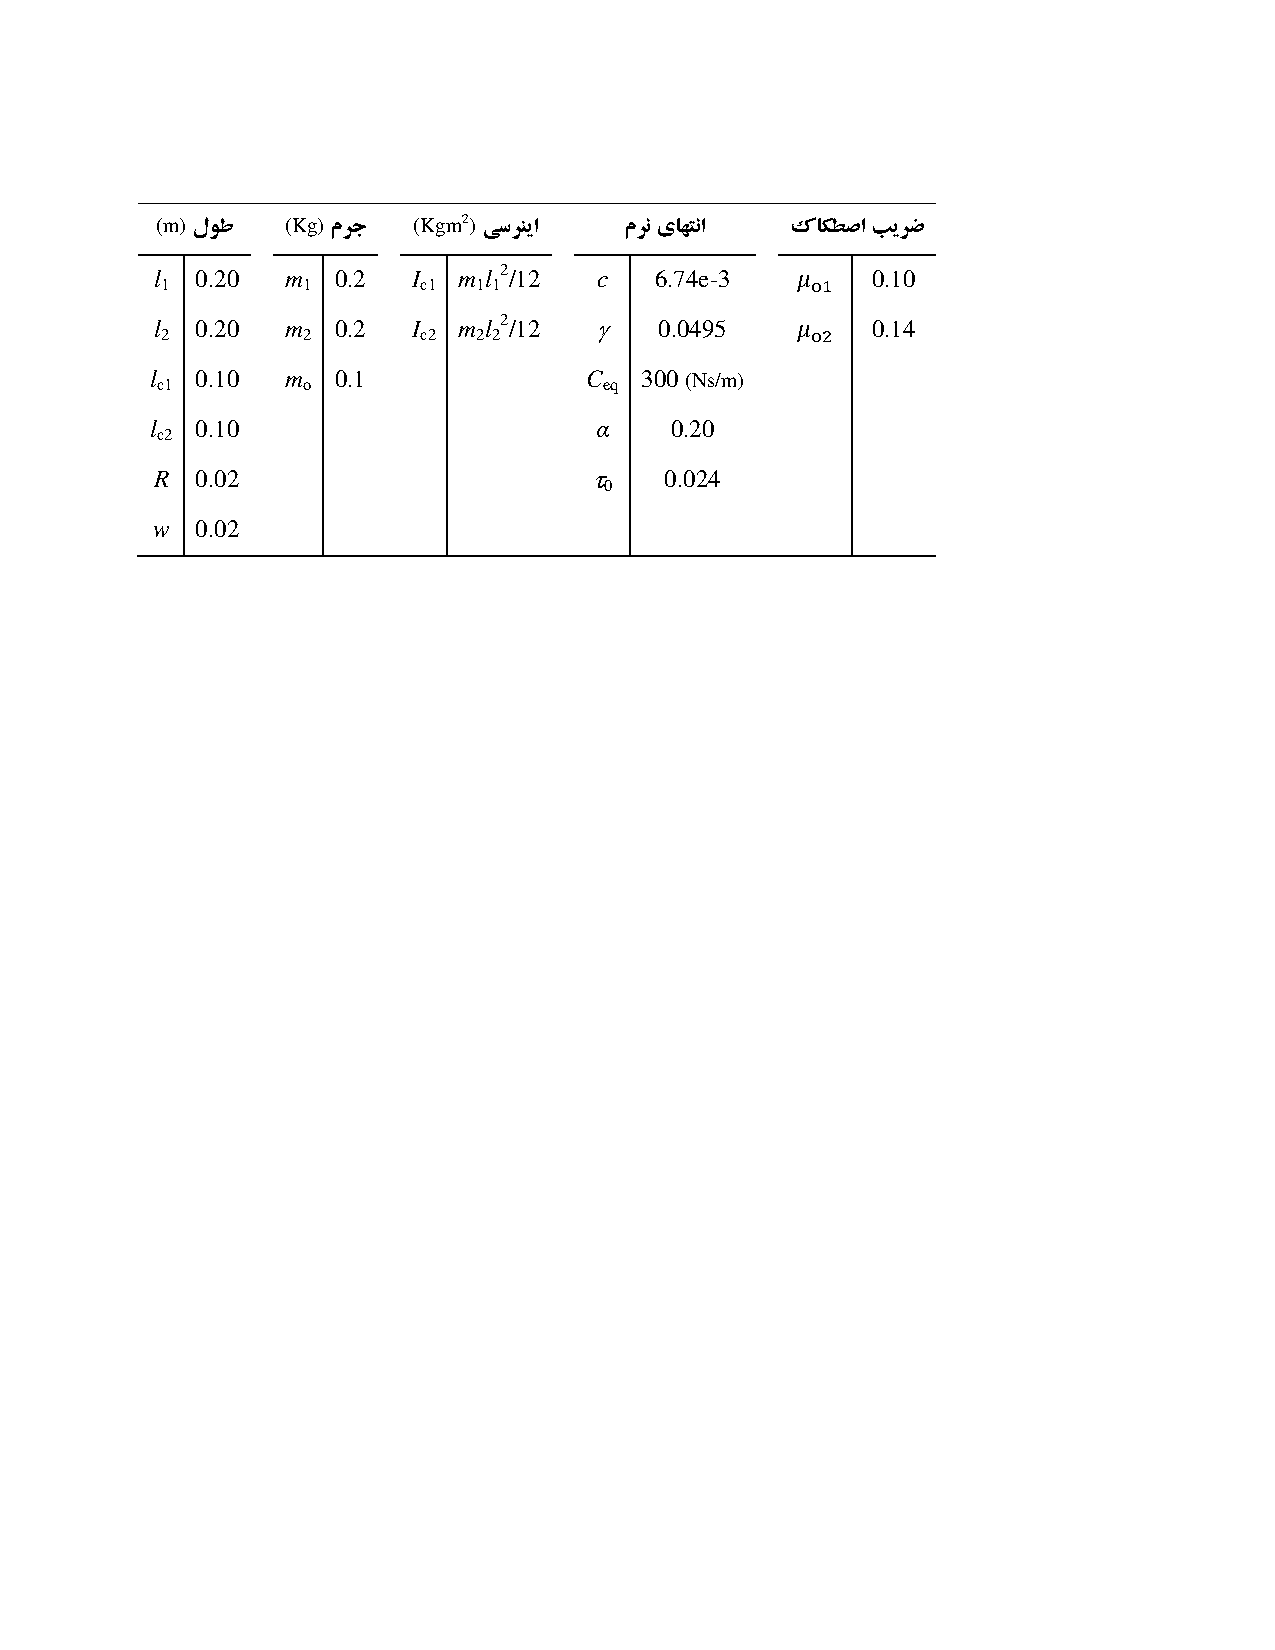
\includegraphics[scale=0.9]{Figures/SampleTable1.pdf} 
\end{tabular}
\vspace{-\baselineskip}
\label{Tbl:SampleTable1_2}
\end{table}

\begin{table}[!htb]
\caption{مقايسه‌ی روش‌هاي برداشت انرژي مبتني بر لرزش‌هاي مکانيکی}
\centering
\begin{tabular}{@{}|p{.15\textwidth}|p{.25\textwidth}|p{.25\textwidth}|p{.25\textwidth}|@{}}
\hline
روش
& 
چگالی انرژی
& 
ابعاد
& 
عیب اصلی
\\ \hline \hline
پیزوالکتریک
& 
$\mathrm{mJ/cm^3}$ 35/4
& 
بزرگ
& 
ولتاژ خروجی کم
\\ \hline
الکترومغناطیس
& 
$\mathrm{mJ/cm^3}$ 24/8
& 
بزرگ
& 
ولتاژ خروجی بسیار کم
\\ \hline
الکترواستاتیک
& 
$\mathrm{mJ/cm^3}$ 4
& 
فشرده در تراشه‌ها
& 
نیاز به منبع شارژ اولیه
\\ \hline
\end{tabular}
\label{Tbl:SampleTable2_2}
\vspace{-\baselineskip}
\end{table}

نمونه‌ای از یک رابطه به‌صورت
\begin{equation}
p\left( r \right) = {C_k}\frac{N}{{\pi {a^2}}}{\left[{1 - {{\left( {\frac{r}{a}} \right)}^k}} \right]^{\frac{1}{k}}},
\label{Eq:Pressure_2}
\end{equation}
است. در رابطه
\ref{Eq:Pressure_2}،
$N$
نیروی عمودی است. نمونه‌ای از استفاده از روابط متوالی به‌صورت
\begin{equation}
\sum \limits_{i = 1}^{k + 1} {E_s}\left( i \right) - T \sum \limits_{i = 1}^k {P_s}\left( i \right) \le B_s^{max},\quad k = 1, \ldots ,N - 1,
\label{Eq:batterysource_2}
\end{equation}\vspace{-\baselineskip}
\begin{equation}
\sum \limits_{i = 1}^{k + 1} {E_r}\left( i \right) - T \sum \limits_{i = 1}^k {P_r}\left( i \right) \le B_r^{max},\quad k = 1, \ldots ,N - 1,
\label{Eq:batteryrellay_2}
\end{equation}
است. نمونه‌ای از یک قضیه و تبصره نیز در ادامه آورده شده است.
\begin{theorem}
اگر ظرفیت باتری‌ها به اندازه کافی بزرگ باشد، جواب بهینه‌ی 
$P_s^*(i)$
و
$P_r^*(i)$
وجود دارد به نحوی که تابع هدف را بیشینه می‌کند و در رابطه‌ی زیر صدق می‌کند:
\begin{equation}
C\left( {{{\left| {{h_{sr}}\left( i \right)} \right|}^2}{P_s}^*\left( i \right)} \right) \ge C\left( {{{\left| {{h_{sd}}\left( i \right)} \right|}^2}{P_s}^*\left( i \right)} \right) + C\left( {{{\left| {{h_{rd}}\left( {i + 1} \right)} \right|}^2}P_r^*\left( {i} \right)} \right).
\label{Eq:theorem1_2}
\end{equation}

\begin{proof}
بار دیگر فرم تابع هدف را در نظر می‌گیریم. لازم به ذکر است اینجا تابع هدف یک تابع دومتغیره است.
\begin{equation}
{R({\mathbf{P}_s},{\mathbf{P}_r}) = {\frac{1}{2}\sum\limits_{i = 1}^N {\min } \left\{ {C\left( {{{\left| {{h_{sr}}\left( i \right)} \right|}^2}{P_s}\left( i \right)} \right),} C\left( {{{\left| {{h_{sd}}\left( i \right)} \right|}^2}{P_s}\left( i \right)} \right) \right\} }}.
\end{equation}
حال بلوک
$i$ام
را در نظر می‌گیریم. اگر رابطه‌ی
\ref{Eq:theorem1_2}
برای
$i$
برقرار نباشد، به عبارت دیگر اگر داشته باشیم،
\begin{equation}
C\left( {{{\left| {{h_{sr}}\left( i \right)} \right|}^2}{P_s}^*\left( i \right)} \right) < C\left( {{{\left| {{h_{sd}}\left( i \right)} \right|}^2}{P_s}^*\left( i \right)} \right) + C\left( {{{\left| {{h_{rd}}\left( {i + 1} \right)} \right|}^2}P_r^*\left( {i + 1} \right)} \right),
\label{Eq:theorem1(2)_2}
\end{equation}
بنابراین
\begin{equation}
C\left( {{{\left| {{h_{sr}}\left( i \right)} \right|}^2}{P_s}^*\left( i \right)} \right)+ C\left( {{{\left| {{h_{sd}}\left( i \right)} \right|}^2}{P_s}^*\left( i \right)} \right) =C\left( {{{\left| {{h_{sr}}\left( i \right)} \right|}^2}{P_s}^*\left( i \right)} \right).
\end{equation}
پس در تابع هدف مسئله، مقدار بهینه‌ی مسئله برابر عبارت سمت چپ رابطه‌ی
\ref{Eq:theorem1(2)_2}
شده است و آرگومان دوم و  هم‌چنین مقدار
$P_r^*(i)$
هیچ نقشی در مقدار بهینه ندارد. بنابراین می‌توانیم 
$P_r^*(i)$
را آنقدر کاهش دهیم تا در رابطه‌ی
\ref{Eq:theorem1(2)_2}
تساوی برقرار شود بدون آنکه مقدار بهینه‌ی مسئله تغییر کند.
\end{proof}
\label{theorem1_2}
\end{theorem}

\begin{remark}
از قضیه‌ی
\ref{theorem1_2}
نتیجه می‌گیریم که جواب بهینه‌ی مسئله‌ی
\lr{P}
در حالت کلی یکتا نیست. به طور مثال وقتی مقدار انرژی برداشت‌شده در رله خیلی بیشتر از این انرژی در منبع باشد مسئله می‌تواند جواب‌های زیادی داشته باشد. بنابراین همواره می‌توان برای صرفه‌جویی در مصرف انرژی، بدون کاهش مقدار نرخ گذردهی سیستم، کمترین مقدار توان را برای رله انتخاب کرد. بنابراین با توجه به رابطه
\begin{equation}
C\left( {{{\left| {{h_{sr}}\left( i \right)} \right|}^2}{P_s}^*\left( i \right)} \right) 
\ge C\left( {{{\left| {{h_{sd}}\left( i \right)} \right|}^2}{P_s}^*\left( i \right)} \right) + C\left( {{{\left| {{h_{rd}}\left( {i} \right)} \right|}^2}P_r^*\left( {i} \right)} \right),
\label{Eq:remark1_2}
\end{equation}
و با  استفاده از رابطه
\ref{Eq:remark1_2}
خواهیم داشت،
\begin{equation}
{R_r}(i) = \min \left\{ {C\left( {{{\left| {{h_{rd}}(i)} \right|}^2}{P_r}(i)} \right),C\left( {{{\left| {{h_{sr}}(i)} \right|}^2}{P_s}(i)} \right)} \right\}.
\end{equation}

بنابراین می‌توان با انتخاب کمترین توان و نرخ برای رله از مصرف بی‌رویه‌ی انرژی جلوگیری کرد. فرض بزرگ بودن ظرفیت باتری‌ به این دلیل است که اگر ظرفیت باتری محدود باشد برای کاهش
$P_r^*(i)$
با محدودیت مواجه هستیم. چون در صورت کاهش بی از حد توان رله ممکن است از ناحیه‌ی شدنی مسئله خارج شویم. به هر حال برای هر دو حالت ظرفیت نامحدود و محدود باتری جواب مسئله یکتا نیست و همواره می‌توان با کاهش توان رله مصرف انرژی را کاهش داد.
\end{remark}




\section{پیش‌گفتار}
در این قالب سعی شده است که از تمامی بخش‌های موجود در پایان‌نامه‌ها نمونه‌ای آورده شود. در این قالب سعی شده است که از تمامی بخش‌های موجود در پایان‌نامه‌ها نمونه‌ای آورده شود. در این قالب سعی شده است که از تمامی بخش‌های موجود در پایان‌نامه‌ها نمونه‌ای آورده شود. در این قالب سعی شده است که از تمامی بخش‌های موجود در پایان‌نامه‌ها نمونه‌ای آورده شود. در این قالب سعی شده است که از تمامی بخش‌های موجود در پایان‌نامه‌ها نمونه‌ای آورده شود. در این قالب سعی شده است که از تمامی بخش‌های موجود در پایان‌نامه‌ها نمونه‌ای آورده شود. در این قالب سعی شده است که از تمامی بخش‌های موجود در پایان‌نامه‌ها نمونه‌ای آورده شود. در این قالب سعی شده است که از تمامی بخش‌های موجود در پایان‌نامه‌ها نمونه‌ای آورده شود. در این قالب سعی شده است که از تمامی بخش‌های موجود در پایان‌نامه‌ها نمونه‌ای آورده شود. در این قالب سعی شده است که از تمامی بخش‌های موجود در پایان‌نامه‌ها نمونه‌ای آورده شود. در این قالب سعی شده است که از تمامی بخش‌های موجود در پایان‌نامه‌ها نمونه‌ای آورده شود. در این قالب سعی شده است که از تمامی بخش‌های موجود در پایان‌نامه‌ها نمونه‌ای آورده شود. در این قالب سعی شده است که از تمامی بخش‌های موجود در پایان‌نامه‌ها نمونه‌ای آورده شود. در این قالب سعی شده است که از تمامی بخش‌های موجود در پایان‌نامه‌ها نمونه‌ای آورده شود.
\section{بخش اول}
نمونه‌ای از یک عبارت انگلیسی در متن به‌صورت
\lr{English Sentence}
است. نمونه‌ای از یک عبارت ریاضی در متن نیز به‌صورت
$x^2 + y^2$
است. ارجاع به مراجع انگلیسی
\cite{Fakhari2015a,Lewis2003}.
ارجاع به مراجع فارسی
\cite{Fakhari2015b,HadianThesis2008}.
این نمونه‌ای از یک زیرنویس انگلیسی%
\LTRfootnote{English Footnote}
است. این نمونه‌ای از یک زیرنویس فارسی%
\RTLfootnote{زیرنویس فارسی}
است. در شکل
\ref{Fig:SampleFigure1_2}،
نمونه‌ای از یک شکل آورده شده است. 

\begin{figure}[!htb]
\centering
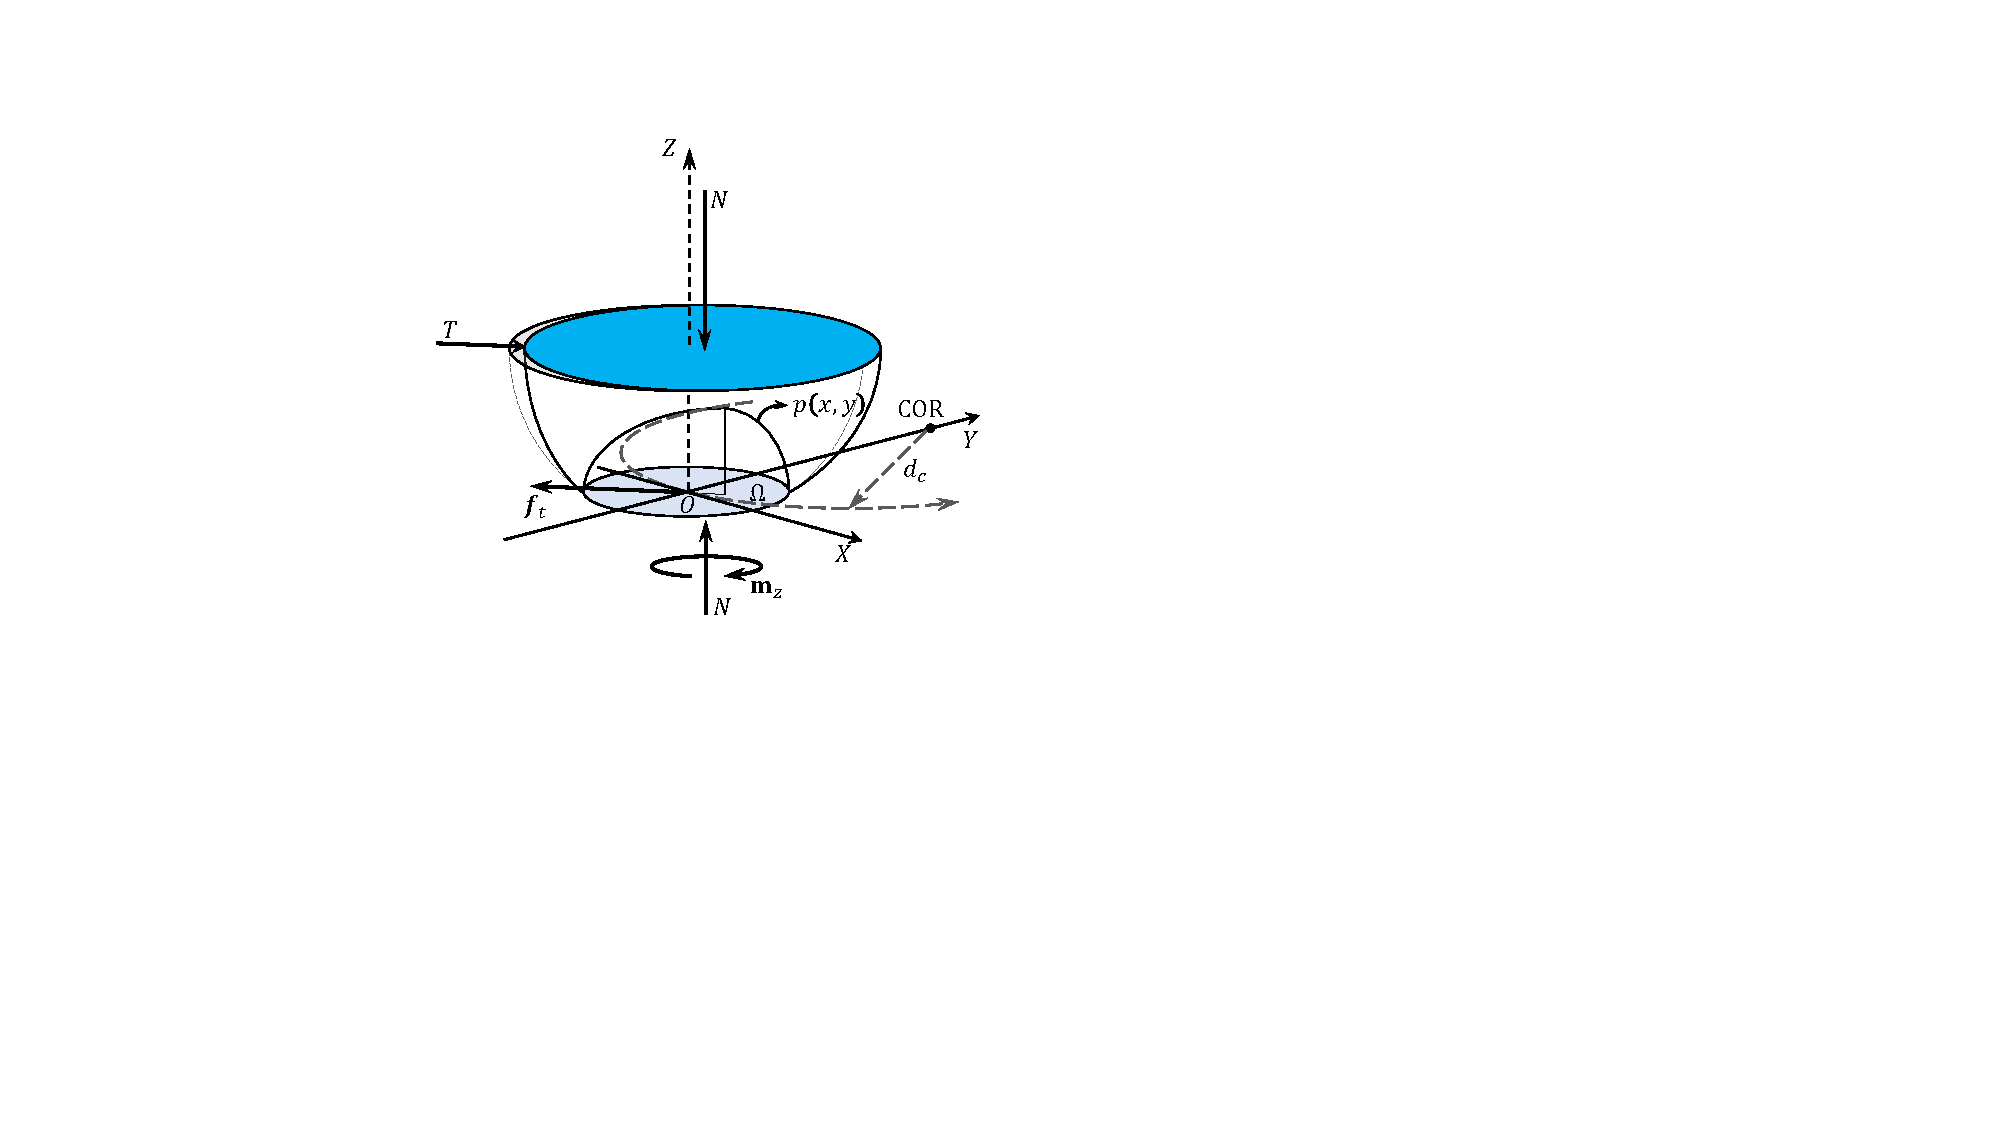
\includegraphics[scale=1]{Figures/SampleFigure.pdf}
\caption{شکل نمونه}
\label{Fig:SampleFigure1_2}
\end{figure}

نمونه‌ای از قرار دادن دو شکل در کنار یکدیگر در شکل
\ref{Fig:SampleFigure2_2}
آورده شده است.

\begin{figure}[!htb]
\centering
\subfloat[زیرنویس شکل اول]{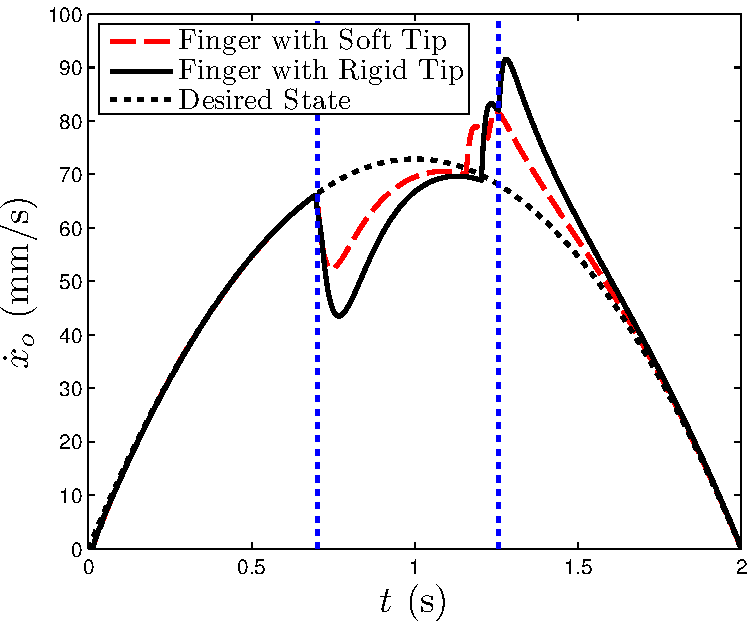
\includegraphics[scale=0.56]{Figures/FigureA.pdf}}
\quad
\subfloat[زیرنویس شکل دوم]{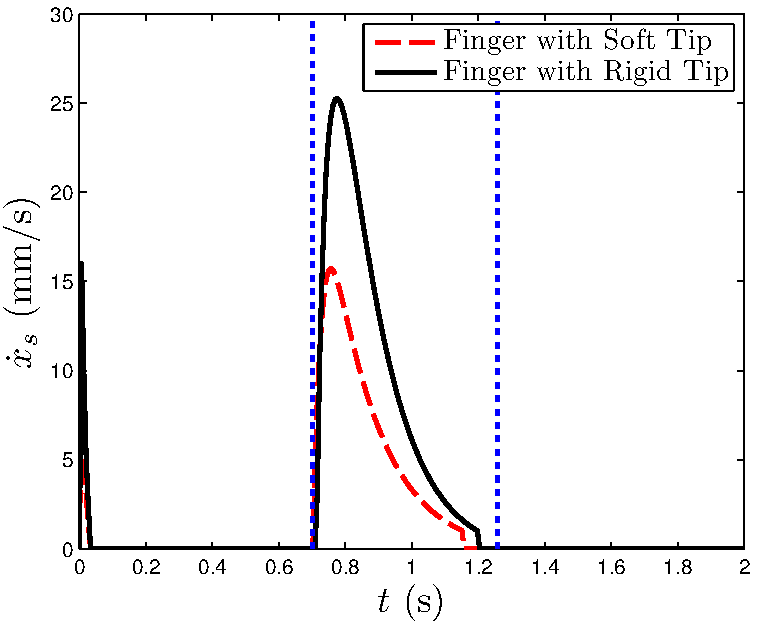
\includegraphics[scale=0.56]{Figures/FigureB.pdf}}
\caption{
قرار دادن دو شکل در کنار یکدیگر، الف) شکل نمونه اول،
ب) شکل نمونه دوم
}
\label{Fig:SampleFigure2_2}
\end{figure}





آیتم‌های مختلف به‌صورت زیر آورده می‌شود:
\begin{itemize}[label=-]
\item
مورد اول
\item
مورد دوم
\item
مورد سوم
\end{itemize}

نمونه‌ای از آیتم‌های شماره‌دار نیز در ادامه آورده شده است. به طور کلی معماری برداشت انرژی به دو دسته‌ی کلی تقسیم می‌شود:
\begin{enumerate}[label=\arabic*)]
\item
برداشت-استفاده:

در این حالت سیستم بلافاصله انرژی برداشت‌شده را مصرف می‌کند. واضح است اگر انرژی کافی در محیط وجود نداشته باشد دستگاه از کار می‌افتد. این نوع سیستم‌ها بیشتر در فشار دادن کلید‌ها، پدال‌ها و دستگاه‌های ردیابی برای انسان‌ها استفاده می‌شود. به طور مثال در پاشنه‌ی کفش دونده‌ای مواد پیزوالکتریک کار گذاشته می‌شود و با فشار پا بر روی کفش و فشرده شدن پیزوالکتریک داخل کفش، انرژی الکتریکی برای ارسال سیگنال 
\lr{RF}
و در نتیجه ردیابی دونده تامین می‌شود. 
\item
برداشت-ذخیره-استفاده:

در این روش سیستم برای ذخیره‌ی انرژی برداشت‌شده به باتری مجهز شده است. این روش برای زمانی‌که انرژی زیادی در محیط وجود داشته باشد و برای منابعی مانند انرژی خورشیدی  کاربرد دارد. روش‌های زیادی برای تبدیل انرژی خورشیدی به انرژی الکتریکی از جمله سلول‌های خورشیدی وجود دارد. در این حالت چگونگی ذخیره‌ی انرژی و بهینه‌سازی مصرف انرژی مطرح می‌شود.
\end{enumerate}




\subsection{زیربخش اول}
نوشته نمونه نوشته نمونه نوشته نمونه نوشته نمونه نوشته نمونه نوشته نمونه نوشته نمونه نوشته نمونه نوشته نمونه نوشته نمونه نوشته نمونه نوشته نمونه نوشته نمونه نوشته نمونه نوشته نمونه نوشته نمونه نوشته نمونه نوشته نمونه نوشته نمونه نوشته نمونه نوشته نمونه نوشته نمونه. در جدول
\ref{Tbl:SampleTable1_2}،
نمونه‌ای از یک جدول واردشده در لاتک و در جدول
\ref{Tbl:SampleTable2_2}،
نمونه‌ای از یک جدول نوشته‌شده در لاتک آورده شده است.

\begin{table}[!htb]
\caption{پارامترهای شبیه‌سازی}
\centering
\begin{tabular}{c}
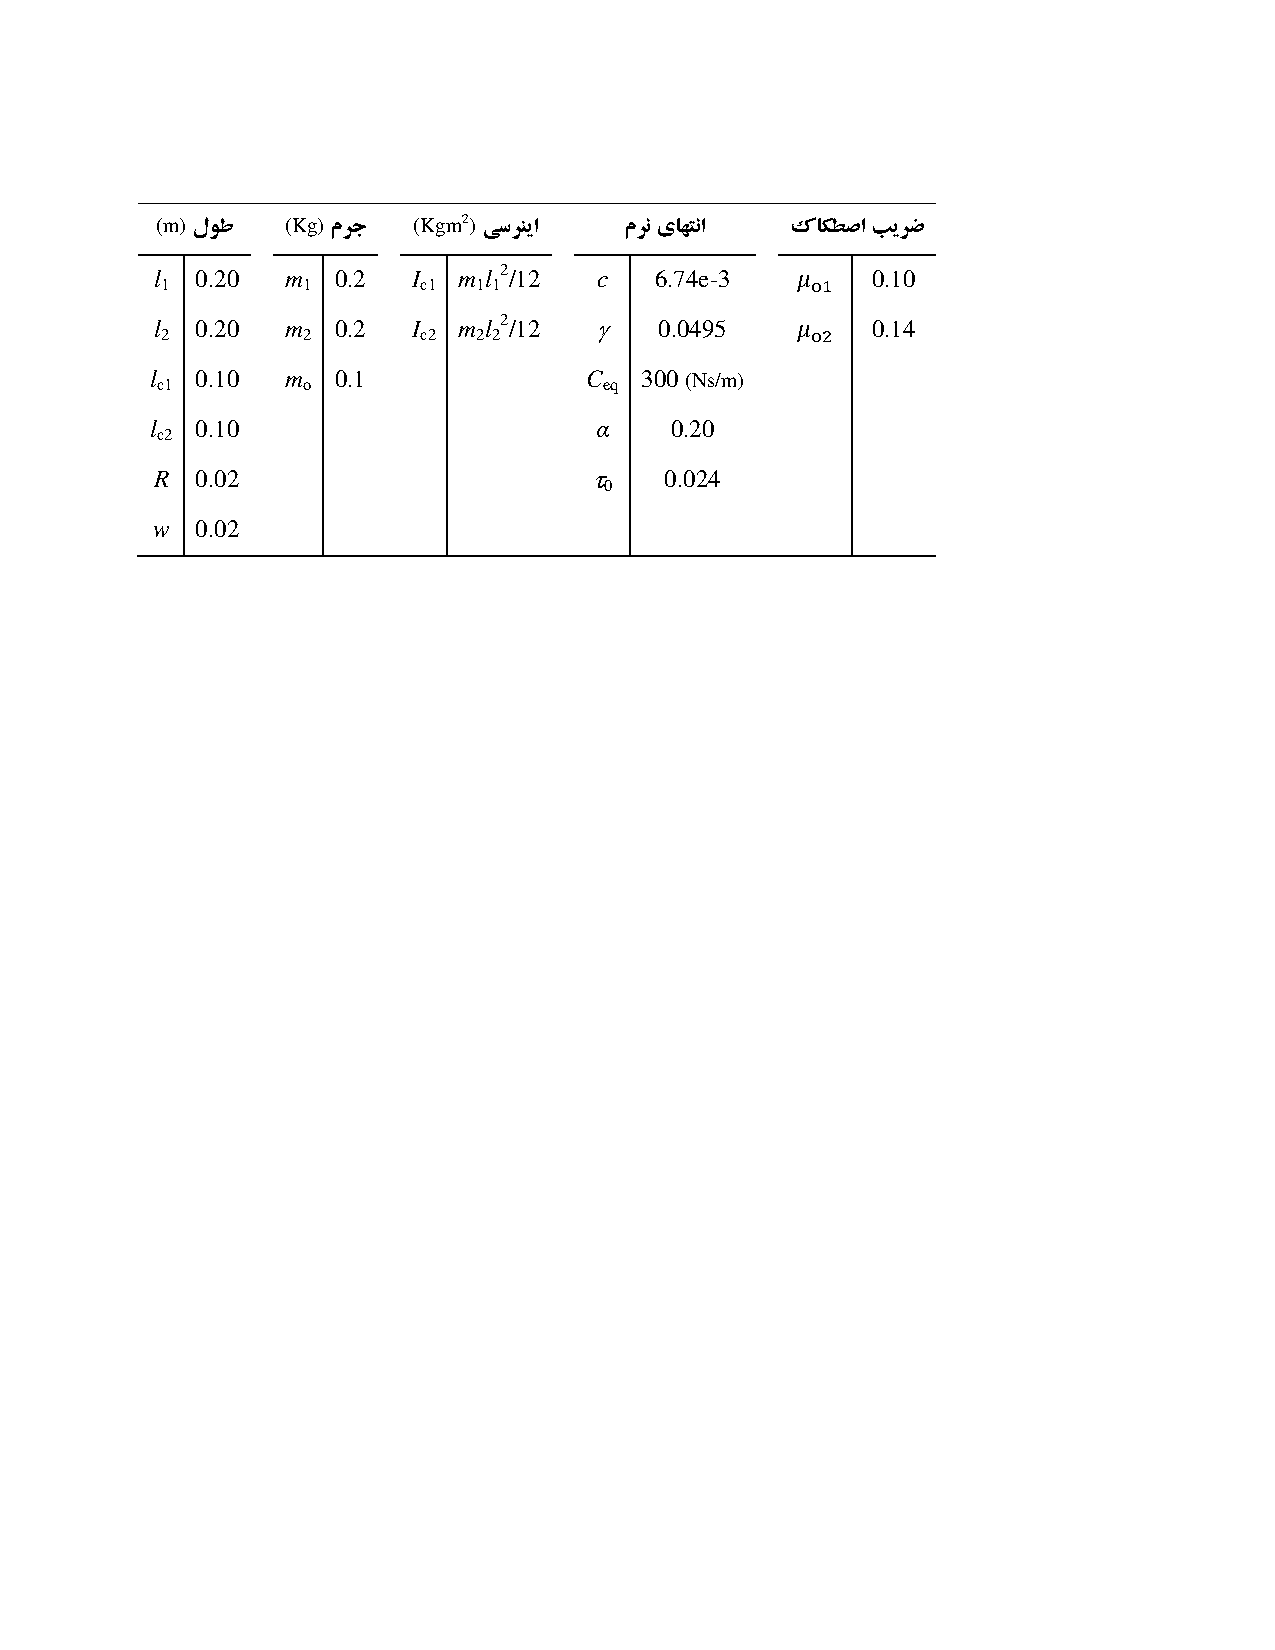
\includegraphics[scale=0.9]{Figures/SampleTable1.pdf} 
\end{tabular}
\vspace{-\baselineskip}
\label{Tbl:SampleTable1_2}
\end{table}

\begin{table}[!htb]
\caption{مقايسه‌ی روش‌هاي برداشت انرژي مبتني بر لرزش‌هاي مکانيکی}
\centering
\begin{tabular}{@{}|p{.15\textwidth}|p{.25\textwidth}|p{.25\textwidth}|p{.25\textwidth}|@{}}
\hline
روش
& 
چگالی انرژی
& 
ابعاد
& 
عیب اصلی
\\ \hline \hline
پیزوالکتریک
& 
$\mathrm{mJ/cm^3}$ 35/4
& 
بزرگ
& 
ولتاژ خروجی کم
\\ \hline
الکترومغناطیس
& 
$\mathrm{mJ/cm^3}$ 24/8
& 
بزرگ
& 
ولتاژ خروجی بسیار کم
\\ \hline
الکترواستاتیک
& 
$\mathrm{mJ/cm^3}$ 4
& 
فشرده در تراشه‌ها
& 
نیاز به منبع شارژ اولیه
\\ \hline
\end{tabular}
\label{Tbl:SampleTable2_2}
\vspace{-\baselineskip}
\end{table}

نمونه‌ای از یک رابطه به‌صورت
\begin{equation}
p\left( r \right) = {C_k}\frac{N}{{\pi {a^2}}}{\left[{1 - {{\left( {\frac{r}{a}} \right)}^k}} \right]^{\frac{1}{k}}},
\label{Eq:Pressure_2}
\end{equation}
است. در رابطه
\ref{Eq:Pressure_2}،
$N$
نیروی عمودی است. نمونه‌ای از استفاده از روابط متوالی به‌صورت
\begin{equation}
\sum \limits_{i = 1}^{k + 1} {E_s}\left( i \right) - T \sum \limits_{i = 1}^k {P_s}\left( i \right) \le B_s^{max},\quad k = 1, \ldots ,N - 1,
\label{Eq:batterysource_2}
\end{equation}\vspace{-\baselineskip}
\begin{equation}
\sum \limits_{i = 1}^{k + 1} {E_r}\left( i \right) - T \sum \limits_{i = 1}^k {P_r}\left( i \right) \le B_r^{max},\quad k = 1, \ldots ,N - 1,
\label{Eq:batteryrellay_2}
\end{equation}
است. نمونه‌ای از یک قضیه و تبصره نیز در ادامه آورده شده است.
\begin{theorem}
اگر ظرفیت باتری‌ها به اندازه کافی بزرگ باشد، جواب بهینه‌ی 
$P_s^*(i)$
و
$P_r^*(i)$
وجود دارد به نحوی که تابع هدف را بیشینه می‌کند و در رابطه‌ی زیر صدق می‌کند:
\begin{equation}
C\left( {{{\left| {{h_{sr}}\left( i \right)} \right|}^2}{P_s}^*\left( i \right)} \right) \ge C\left( {{{\left| {{h_{sd}}\left( i \right)} \right|}^2}{P_s}^*\left( i \right)} \right) + C\left( {{{\left| {{h_{rd}}\left( {i + 1} \right)} \right|}^2}P_r^*\left( {i} \right)} \right).
\label{Eq:theorem1_2}
\end{equation}

\begin{proof}
بار دیگر فرم تابع هدف را در نظر می‌گیریم. لازم به ذکر است اینجا تابع هدف یک تابع دومتغیره است.
\begin{equation}
{R({\mathbf{P}_s},{\mathbf{P}_r}) = {\frac{1}{2}\sum\limits_{i = 1}^N {\min } \left\{ {C\left( {{{\left| {{h_{sr}}\left( i \right)} \right|}^2}{P_s}\left( i \right)} \right),} C\left( {{{\left| {{h_{sd}}\left( i \right)} \right|}^2}{P_s}\left( i \right)} \right) \right\} }}.
\end{equation}
حال بلوک
$i$ام
را در نظر می‌گیریم. اگر رابطه‌ی
\ref{Eq:theorem1_2}
برای
$i$
برقرار نباشد، به عبارت دیگر اگر داشته باشیم،
\begin{equation}
C\left( {{{\left| {{h_{sr}}\left( i \right)} \right|}^2}{P_s}^*\left( i \right)} \right) < C\left( {{{\left| {{h_{sd}}\left( i \right)} \right|}^2}{P_s}^*\left( i \right)} \right) + C\left( {{{\left| {{h_{rd}}\left( {i + 1} \right)} \right|}^2}P_r^*\left( {i + 1} \right)} \right),
\label{Eq:theorem1(2)_2}
\end{equation}
بنابراین
\begin{equation}
C\left( {{{\left| {{h_{sr}}\left( i \right)} \right|}^2}{P_s}^*\left( i \right)} \right)+ C\left( {{{\left| {{h_{sd}}\left( i \right)} \right|}^2}{P_s}^*\left( i \right)} \right) =C\left( {{{\left| {{h_{sr}}\left( i \right)} \right|}^2}{P_s}^*\left( i \right)} \right).
\end{equation}
پس در تابع هدف مسئله، مقدار بهینه‌ی مسئله برابر عبارت سمت چپ رابطه‌ی
\ref{Eq:theorem1(2)_2}
شده است و آرگومان دوم و  هم‌چنین مقدار
$P_r^*(i)$
هیچ نقشی در مقدار بهینه ندارد. بنابراین می‌توانیم 
$P_r^*(i)$
را آنقدر کاهش دهیم تا در رابطه‌ی
\ref{Eq:theorem1(2)_2}
تساوی برقرار شود بدون آنکه مقدار بهینه‌ی مسئله تغییر کند.
\end{proof}
\label{theorem1_2}
\end{theorem}

\begin{remark}
از قضیه‌ی
\ref{theorem1_2}
نتیجه می‌گیریم که جواب بهینه‌ی مسئله‌ی
\lr{P}
در حالت کلی یکتا نیست. به طور مثال وقتی مقدار انرژی برداشت‌شده در رله خیلی بیشتر از این انرژی در منبع باشد مسئله می‌تواند جواب‌های زیادی داشته باشد. بنابراین همواره می‌توان برای صرفه‌جویی در مصرف انرژی، بدون کاهش مقدار نرخ گذردهی سیستم، کمترین مقدار توان را برای رله انتخاب کرد. بنابراین با توجه به رابطه
\begin{equation}
C\left( {{{\left| {{h_{sr}}\left( i \right)} \right|}^2}{P_s}^*\left( i \right)} \right) 
\ge C\left( {{{\left| {{h_{sd}}\left( i \right)} \right|}^2}{P_s}^*\left( i \right)} \right) + C\left( {{{\left| {{h_{rd}}\left( {i} \right)} \right|}^2}P_r^*\left( {i} \right)} \right),
\label{Eq:remark1_2}
\end{equation}
و با  استفاده از رابطه
\ref{Eq:remark1_2}
خواهیم داشت،
\begin{equation}
{R_r}(i) = \min \left\{ {C\left( {{{\left| {{h_{rd}}(i)} \right|}^2}{P_r}(i)} \right),C\left( {{{\left| {{h_{sr}}(i)} \right|}^2}{P_s}(i)} \right)} \right\}.
\end{equation}

بنابراین می‌توان با انتخاب کمترین توان و نرخ برای رله از مصرف بی‌رویه‌ی انرژی جلوگیری کرد. فرض بزرگ بودن ظرفیت باتری‌ به این دلیل است که اگر ظرفیت باتری محدود باشد برای کاهش
$P_r^*(i)$
با محدودیت مواجه هستیم. چون در صورت کاهش بی از حد توان رله ممکن است از ناحیه‌ی شدنی مسئله خارج شویم. به هر حال برای هر دو حالت ظرفیت نامحدود و محدود باتری جواب مسئله یکتا نیست و همواره می‌توان با کاهش توان رله مصرف انرژی را کاهش داد.
\end{remark}




\section{پیش‌گفتار}
در این قالب سعی شده است که از تمامی بخش‌های موجود در پایان‌نامه‌ها نمونه‌ای آورده شود. در این قالب سعی شده است که از تمامی بخش‌های موجود در پایان‌نامه‌ها نمونه‌ای آورده شود. در این قالب سعی شده است که از تمامی بخش‌های موجود در پایان‌نامه‌ها نمونه‌ای آورده شود. در این قالب سعی شده است که از تمامی بخش‌های موجود در پایان‌نامه‌ها نمونه‌ای آورده شود. در این قالب سعی شده است که از تمامی بخش‌های موجود در پایان‌نامه‌ها نمونه‌ای آورده شود. در این قالب سعی شده است که از تمامی بخش‌های موجود در پایان‌نامه‌ها نمونه‌ای آورده شود. در این قالب سعی شده است که از تمامی بخش‌های موجود در پایان‌نامه‌ها نمونه‌ای آورده شود. در این قالب سعی شده است که از تمامی بخش‌های موجود در پایان‌نامه‌ها نمونه‌ای آورده شود. در این قالب سعی شده است که از تمامی بخش‌های موجود در پایان‌نامه‌ها نمونه‌ای آورده شود. در این قالب سعی شده است که از تمامی بخش‌های موجود در پایان‌نامه‌ها نمونه‌ای آورده شود. در این قالب سعی شده است که از تمامی بخش‌های موجود در پایان‌نامه‌ها نمونه‌ای آورده شود. در این قالب سعی شده است که از تمامی بخش‌های موجود در پایان‌نامه‌ها نمونه‌ای آورده شود. در این قالب سعی شده است که از تمامی بخش‌های موجود در پایان‌نامه‌ها نمونه‌ای آورده شود. در این قالب سعی شده است که از تمامی بخش‌های موجود در پایان‌نامه‌ها نمونه‌ای آورده شود.
\section{بخش اول}
نمونه‌ای از یک عبارت انگلیسی در متن به‌صورت
\lr{English Sentence}
است. نمونه‌ای از یک عبارت ریاضی در متن نیز به‌صورت
$x^2 + y^2$
است. ارجاع به مراجع انگلیسی
\cite{Fakhari2015a,Lewis2003}.
ارجاع به مراجع فارسی
\cite{Fakhari2015b,HadianThesis2008}.
این نمونه‌ای از یک زیرنویس انگلیسی%
\LTRfootnote{English Footnote}
است. این نمونه‌ای از یک زیرنویس فارسی%
\RTLfootnote{زیرنویس فارسی}
است. در شکل
\ref{Fig:SampleFigure1_2}،
نمونه‌ای از یک شکل آورده شده است. 

\begin{figure}[!htb]
\centering
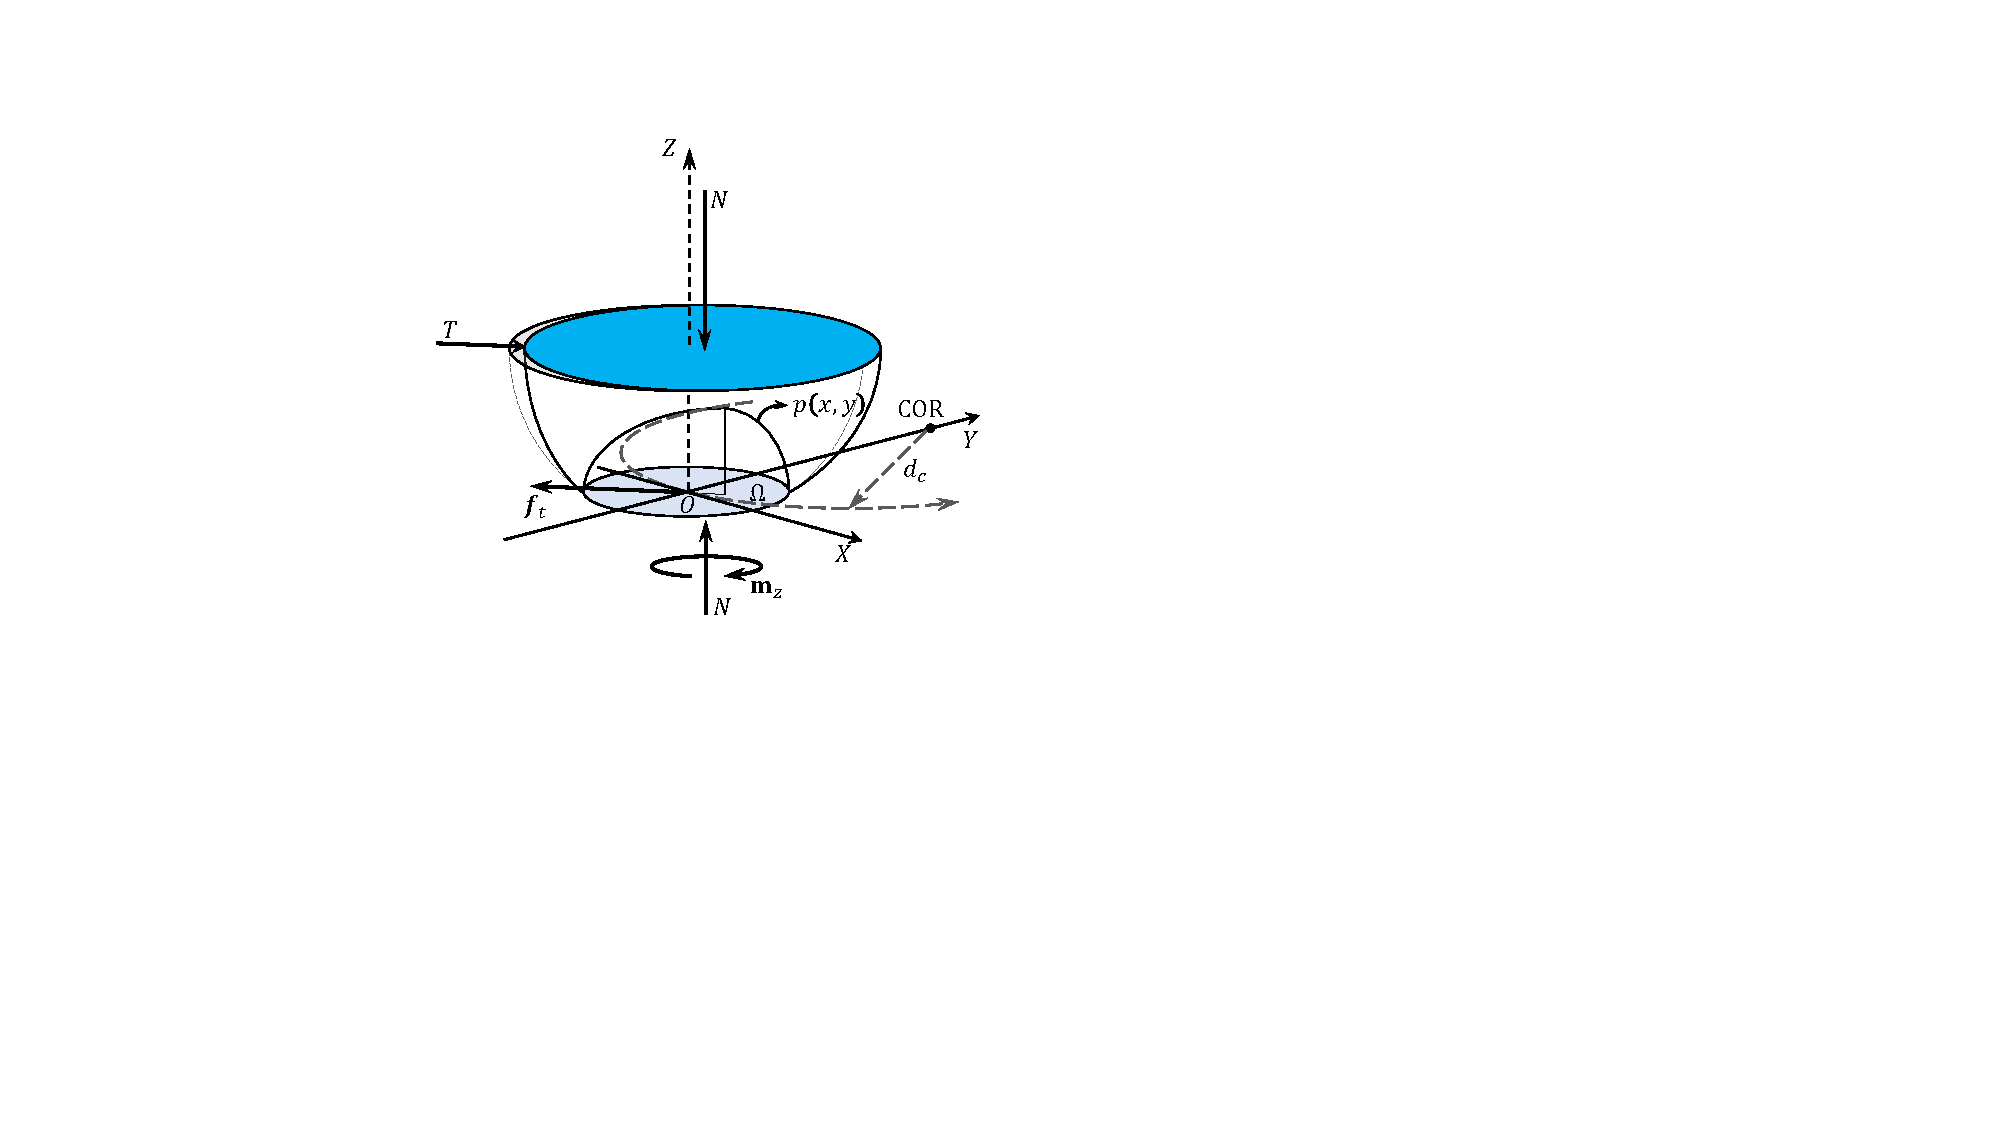
\includegraphics[scale=1]{Figures/SampleFigure.pdf}
\caption{شکل نمونه}
\label{Fig:SampleFigure1_2}
\end{figure}

نمونه‌ای از قرار دادن دو شکل در کنار یکدیگر در شکل
\ref{Fig:SampleFigure2_2}
آورده شده است.

\begin{figure}[!htb]
\centering
\subfloat[زیرنویس شکل اول]{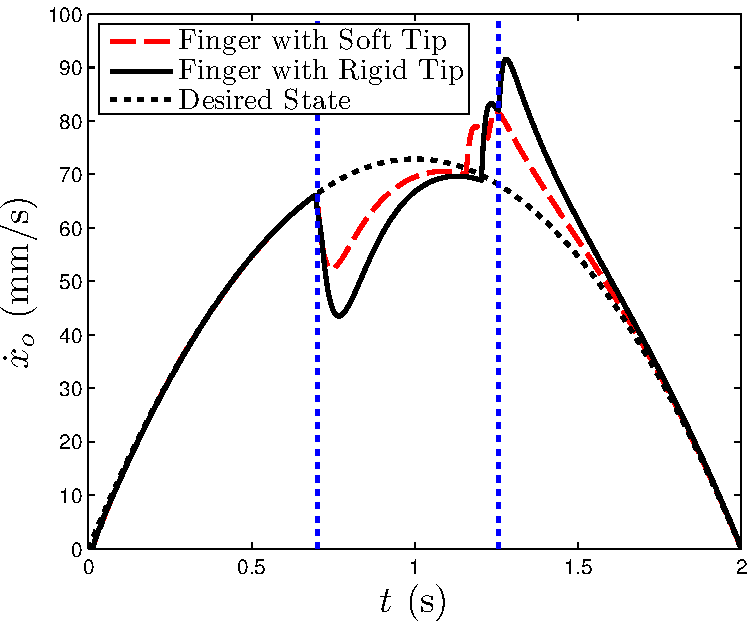
\includegraphics[scale=0.56]{Figures/FigureA.pdf}}
\quad
\subfloat[زیرنویس شکل دوم]{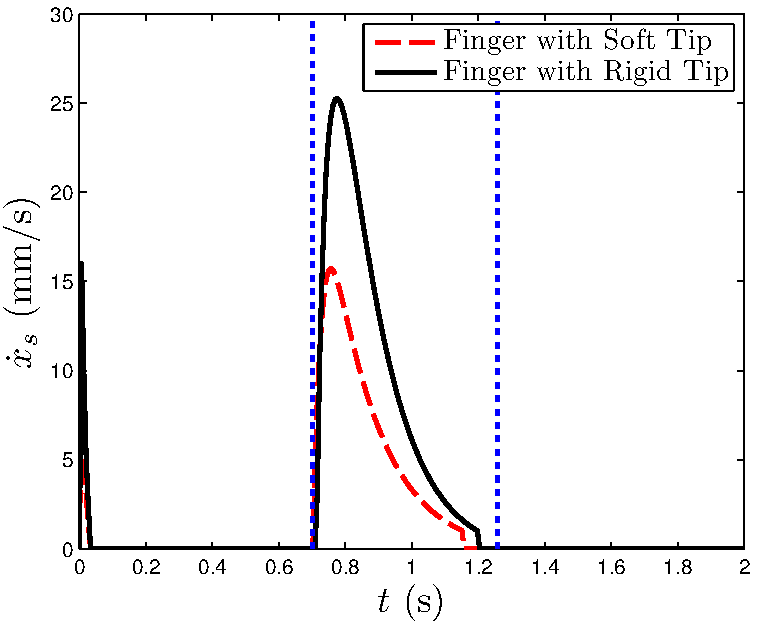
\includegraphics[scale=0.56]{Figures/FigureB.pdf}}
\caption{
قرار دادن دو شکل در کنار یکدیگر، الف) شکل نمونه اول،
ب) شکل نمونه دوم
}
\label{Fig:SampleFigure2_2}
\end{figure}





آیتم‌های مختلف به‌صورت زیر آورده می‌شود:
\begin{itemize}[label=-]
\item
مورد اول
\item
مورد دوم
\item
مورد سوم
\end{itemize}

نمونه‌ای از آیتم‌های شماره‌دار نیز در ادامه آورده شده است. به طور کلی معماری برداشت انرژی به دو دسته‌ی کلی تقسیم می‌شود:
\begin{enumerate}[label=\arabic*)]
\item
برداشت-استفاده:

در این حالت سیستم بلافاصله انرژی برداشت‌شده را مصرف می‌کند. واضح است اگر انرژی کافی در محیط وجود نداشته باشد دستگاه از کار می‌افتد. این نوع سیستم‌ها بیشتر در فشار دادن کلید‌ها، پدال‌ها و دستگاه‌های ردیابی برای انسان‌ها استفاده می‌شود. به طور مثال در پاشنه‌ی کفش دونده‌ای مواد پیزوالکتریک کار گذاشته می‌شود و با فشار پا بر روی کفش و فشرده شدن پیزوالکتریک داخل کفش، انرژی الکتریکی برای ارسال سیگنال 
\lr{RF}
و در نتیجه ردیابی دونده تامین می‌شود. 
\item
برداشت-ذخیره-استفاده:

در این روش سیستم برای ذخیره‌ی انرژی برداشت‌شده به باتری مجهز شده است. این روش برای زمانی‌که انرژی زیادی در محیط وجود داشته باشد و برای منابعی مانند انرژی خورشیدی  کاربرد دارد. روش‌های زیادی برای تبدیل انرژی خورشیدی به انرژی الکتریکی از جمله سلول‌های خورشیدی وجود دارد. در این حالت چگونگی ذخیره‌ی انرژی و بهینه‌سازی مصرف انرژی مطرح می‌شود.
\end{enumerate}




\subsection{زیربخش اول}
نوشته نمونه نوشته نمونه نوشته نمونه نوشته نمونه نوشته نمونه نوشته نمونه نوشته نمونه نوشته نمونه نوشته نمونه نوشته نمونه نوشته نمونه نوشته نمونه نوشته نمونه نوشته نمونه نوشته نمونه نوشته نمونه نوشته نمونه نوشته نمونه نوشته نمونه نوشته نمونه نوشته نمونه نوشته نمونه. در جدول
\ref{Tbl:SampleTable1_2}،
نمونه‌ای از یک جدول واردشده در لاتک و در جدول
\ref{Tbl:SampleTable2_2}،
نمونه‌ای از یک جدول نوشته‌شده در لاتک آورده شده است.

\begin{table}[!htb]
\caption{پارامترهای شبیه‌سازی}
\centering
\begin{tabular}{c}
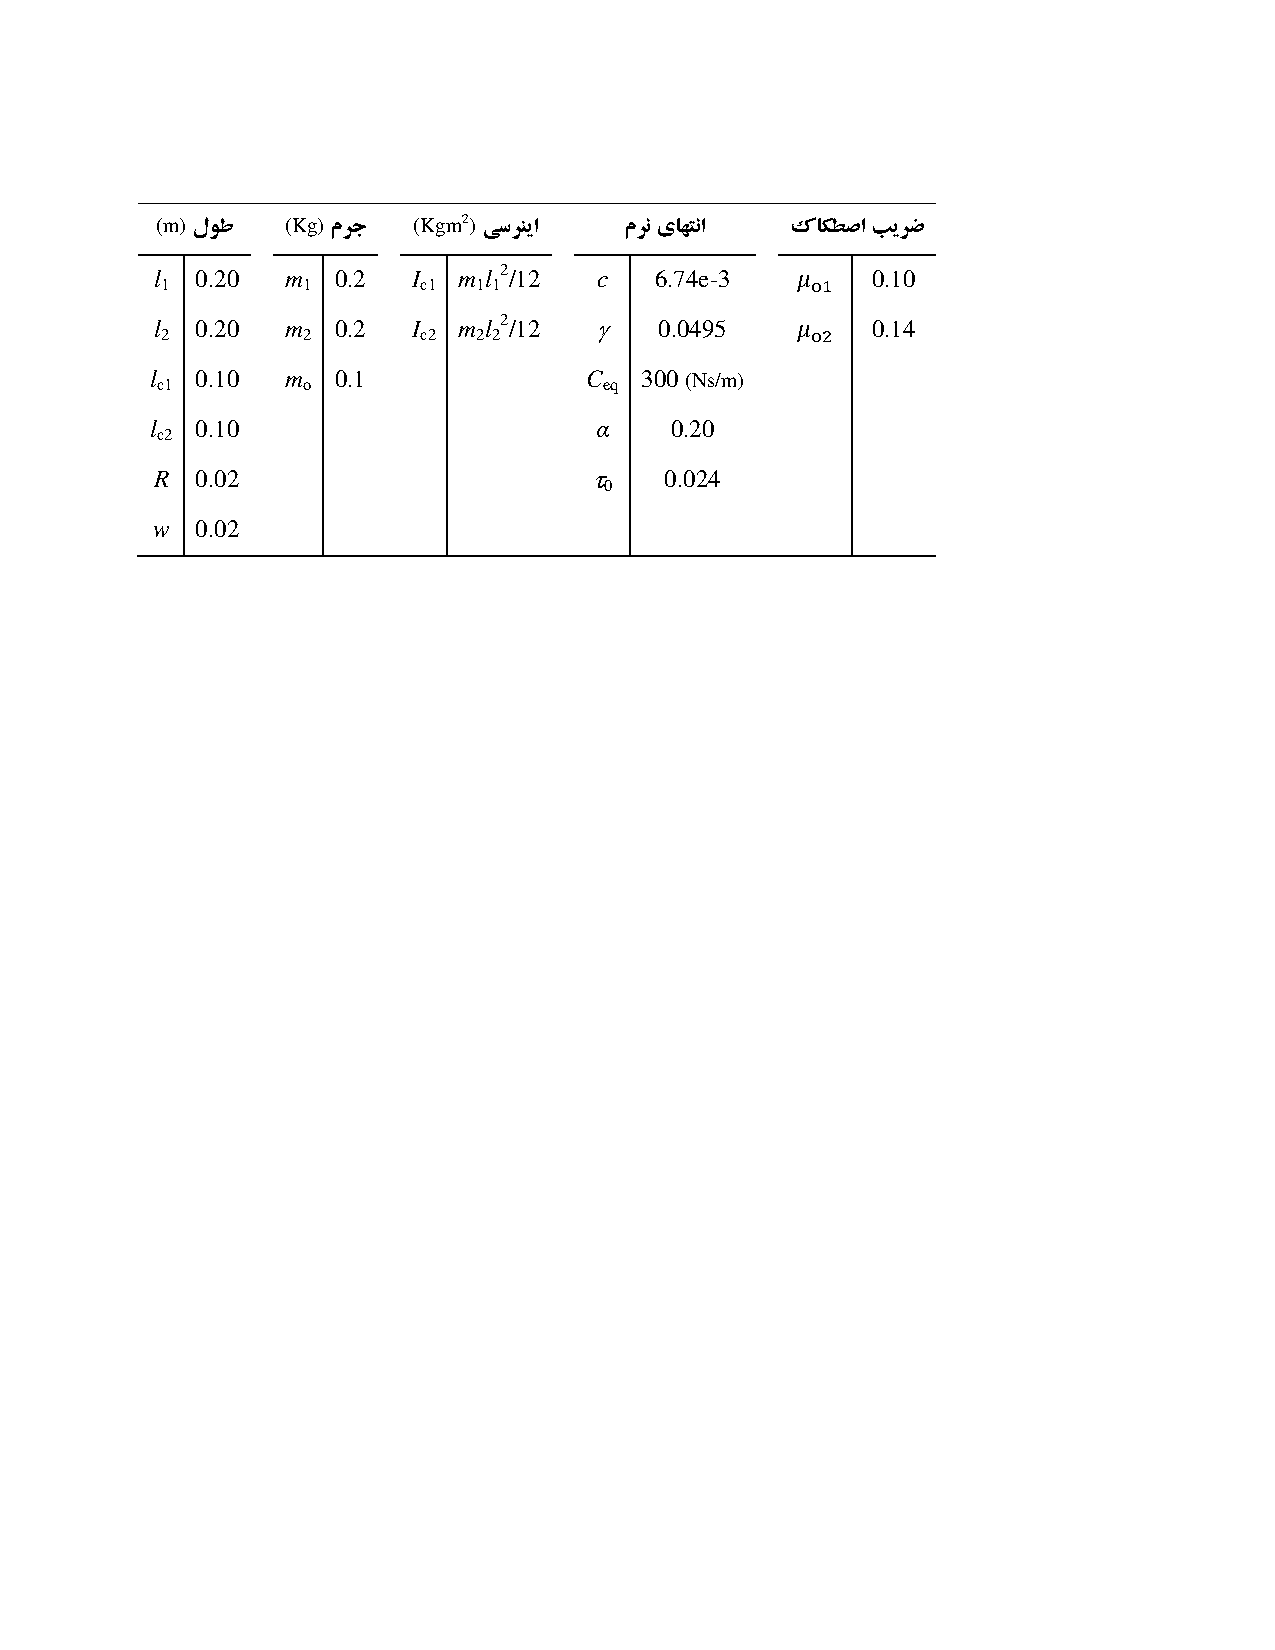
\includegraphics[scale=0.9]{Figures/SampleTable1.pdf} 
\end{tabular}
\vspace{-\baselineskip}
\label{Tbl:SampleTable1_2}
\end{table}

\begin{table}[!htb]
\caption{مقايسه‌ی روش‌هاي برداشت انرژي مبتني بر لرزش‌هاي مکانيکی}
\centering
\begin{tabular}{@{}|p{.15\textwidth}|p{.25\textwidth}|p{.25\textwidth}|p{.25\textwidth}|@{}}
\hline
روش
& 
چگالی انرژی
& 
ابعاد
& 
عیب اصلی
\\ \hline \hline
پیزوالکتریک
& 
$\mathrm{mJ/cm^3}$ 35/4
& 
بزرگ
& 
ولتاژ خروجی کم
\\ \hline
الکترومغناطیس
& 
$\mathrm{mJ/cm^3}$ 24/8
& 
بزرگ
& 
ولتاژ خروجی بسیار کم
\\ \hline
الکترواستاتیک
& 
$\mathrm{mJ/cm^3}$ 4
& 
فشرده در تراشه‌ها
& 
نیاز به منبع شارژ اولیه
\\ \hline
\end{tabular}
\label{Tbl:SampleTable2_2}
\vspace{-\baselineskip}
\end{table}

نمونه‌ای از یک رابطه به‌صورت
\begin{equation}
p\left( r \right) = {C_k}\frac{N}{{\pi {a^2}}}{\left[{1 - {{\left( {\frac{r}{a}} \right)}^k}} \right]^{\frac{1}{k}}},
\label{Eq:Pressure_2}
\end{equation}
است. در رابطه
\ref{Eq:Pressure_2}،
$N$
نیروی عمودی است. نمونه‌ای از استفاده از روابط متوالی به‌صورت
\begin{equation}
\sum \limits_{i = 1}^{k + 1} {E_s}\left( i \right) - T \sum \limits_{i = 1}^k {P_s}\left( i \right) \le B_s^{max},\quad k = 1, \ldots ,N - 1,
\label{Eq:batterysource_2}
\end{equation}\vspace{-\baselineskip}
\begin{equation}
\sum \limits_{i = 1}^{k + 1} {E_r}\left( i \right) - T \sum \limits_{i = 1}^k {P_r}\left( i \right) \le B_r^{max},\quad k = 1, \ldots ,N - 1,
\label{Eq:batteryrellay_2}
\end{equation}
است. نمونه‌ای از یک قضیه و تبصره نیز در ادامه آورده شده است.
\begin{theorem}
اگر ظرفیت باتری‌ها به اندازه کافی بزرگ باشد، جواب بهینه‌ی 
$P_s^*(i)$
و
$P_r^*(i)$
وجود دارد به نحوی که تابع هدف را بیشینه می‌کند و در رابطه‌ی زیر صدق می‌کند:
\begin{equation}
C\left( {{{\left| {{h_{sr}}\left( i \right)} \right|}^2}{P_s}^*\left( i \right)} \right) \ge C\left( {{{\left| {{h_{sd}}\left( i \right)} \right|}^2}{P_s}^*\left( i \right)} \right) + C\left( {{{\left| {{h_{rd}}\left( {i + 1} \right)} \right|}^2}P_r^*\left( {i} \right)} \right).
\label{Eq:theorem1_2}
\end{equation}

\begin{proof}
بار دیگر فرم تابع هدف را در نظر می‌گیریم. لازم به ذکر است اینجا تابع هدف یک تابع دومتغیره است.
\begin{equation}
{R({\mathbf{P}_s},{\mathbf{P}_r}) = {\frac{1}{2}\sum\limits_{i = 1}^N {\min } \left\{ {C\left( {{{\left| {{h_{sr}}\left( i \right)} \right|}^2}{P_s}\left( i \right)} \right),} C\left( {{{\left| {{h_{sd}}\left( i \right)} \right|}^2}{P_s}\left( i \right)} \right) \right\} }}.
\end{equation}
حال بلوک
$i$ام
را در نظر می‌گیریم. اگر رابطه‌ی
\ref{Eq:theorem1_2}
برای
$i$
برقرار نباشد، به عبارت دیگر اگر داشته باشیم،
\begin{equation}
C\left( {{{\left| {{h_{sr}}\left( i \right)} \right|}^2}{P_s}^*\left( i \right)} \right) < C\left( {{{\left| {{h_{sd}}\left( i \right)} \right|}^2}{P_s}^*\left( i \right)} \right) + C\left( {{{\left| {{h_{rd}}\left( {i + 1} \right)} \right|}^2}P_r^*\left( {i + 1} \right)} \right),
\label{Eq:theorem1(2)_2}
\end{equation}
بنابراین
\begin{equation}
C\left( {{{\left| {{h_{sr}}\left( i \right)} \right|}^2}{P_s}^*\left( i \right)} \right)+ C\left( {{{\left| {{h_{sd}}\left( i \right)} \right|}^2}{P_s}^*\left( i \right)} \right) =C\left( {{{\left| {{h_{sr}}\left( i \right)} \right|}^2}{P_s}^*\left( i \right)} \right).
\end{equation}
پس در تابع هدف مسئله، مقدار بهینه‌ی مسئله برابر عبارت سمت چپ رابطه‌ی
\ref{Eq:theorem1(2)_2}
شده است و آرگومان دوم و  هم‌چنین مقدار
$P_r^*(i)$
هیچ نقشی در مقدار بهینه ندارد. بنابراین می‌توانیم 
$P_r^*(i)$
را آنقدر کاهش دهیم تا در رابطه‌ی
\ref{Eq:theorem1(2)_2}
تساوی برقرار شود بدون آنکه مقدار بهینه‌ی مسئله تغییر کند.
\end{proof}
\label{theorem1_2}
\end{theorem}

\begin{remark}
از قضیه‌ی
\ref{theorem1_2}
نتیجه می‌گیریم که جواب بهینه‌ی مسئله‌ی
\lr{P}
در حالت کلی یکتا نیست. به طور مثال وقتی مقدار انرژی برداشت‌شده در رله خیلی بیشتر از این انرژی در منبع باشد مسئله می‌تواند جواب‌های زیادی داشته باشد. بنابراین همواره می‌توان برای صرفه‌جویی در مصرف انرژی، بدون کاهش مقدار نرخ گذردهی سیستم، کمترین مقدار توان را برای رله انتخاب کرد. بنابراین با توجه به رابطه
\begin{equation}
C\left( {{{\left| {{h_{sr}}\left( i \right)} \right|}^2}{P_s}^*\left( i \right)} \right) 
\ge C\left( {{{\left| {{h_{sd}}\left( i \right)} \right|}^2}{P_s}^*\left( i \right)} \right) + C\left( {{{\left| {{h_{rd}}\left( {i} \right)} \right|}^2}P_r^*\left( {i} \right)} \right),
\label{Eq:remark1_2}
\end{equation}
و با  استفاده از رابطه
\ref{Eq:remark1_2}
خواهیم داشت،
\begin{equation}
{R_r}(i) = \min \left\{ {C\left( {{{\left| {{h_{rd}}(i)} \right|}^2}{P_r}(i)} \right),C\left( {{{\left| {{h_{sr}}(i)} \right|}^2}{P_s}(i)} \right)} \right\}.
\end{equation}

بنابراین می‌توان با انتخاب کمترین توان و نرخ برای رله از مصرف بی‌رویه‌ی انرژی جلوگیری کرد. فرض بزرگ بودن ظرفیت باتری‌ به این دلیل است که اگر ظرفیت باتری محدود باشد برای کاهش
$P_r^*(i)$
با محدودیت مواجه هستیم. چون در صورت کاهش بی از حد توان رله ممکن است از ناحیه‌ی شدنی مسئله خارج شویم. به هر حال برای هر دو حالت ظرفیت نامحدود و محدود باتری جواب مسئله یکتا نیست و همواره می‌توان با کاهش توان رله مصرف انرژی را کاهش داد.
\end{remark}




\section{پیش‌گفتار}
در این قالب سعی شده است که از تمامی بخش‌های موجود در پایان‌نامه‌ها نمونه‌ای آورده شود. در این قالب سعی شده است که از تمامی بخش‌های موجود در پایان‌نامه‌ها نمونه‌ای آورده شود. در این قالب سعی شده است که از تمامی بخش‌های موجود در پایان‌نامه‌ها نمونه‌ای آورده شود. در این قالب سعی شده است که از تمامی بخش‌های موجود در پایان‌نامه‌ها نمونه‌ای آورده شود. در این قالب سعی شده است که از تمامی بخش‌های موجود در پایان‌نامه‌ها نمونه‌ای آورده شود. در این قالب سعی شده است که از تمامی بخش‌های موجود در پایان‌نامه‌ها نمونه‌ای آورده شود. در این قالب سعی شده است که از تمامی بخش‌های موجود در پایان‌نامه‌ها نمونه‌ای آورده شود. در این قالب سعی شده است که از تمامی بخش‌های موجود در پایان‌نامه‌ها نمونه‌ای آورده شود. در این قالب سعی شده است که از تمامی بخش‌های موجود در پایان‌نامه‌ها نمونه‌ای آورده شود. در این قالب سعی شده است که از تمامی بخش‌های موجود در پایان‌نامه‌ها نمونه‌ای آورده شود. در این قالب سعی شده است که از تمامی بخش‌های موجود در پایان‌نامه‌ها نمونه‌ای آورده شود. در این قالب سعی شده است که از تمامی بخش‌های موجود در پایان‌نامه‌ها نمونه‌ای آورده شود. در این قالب سعی شده است که از تمامی بخش‌های موجود در پایان‌نامه‌ها نمونه‌ای آورده شود. در این قالب سعی شده است که از تمامی بخش‌های موجود در پایان‌نامه‌ها نمونه‌ای آورده شود.
\section{بخش اول}
نمونه‌ای از یک عبارت انگلیسی در متن به‌صورت
\lr{English Sentence}
است. نمونه‌ای از یک عبارت ریاضی در متن نیز به‌صورت
$x^2 + y^2$
است. ارجاع به مراجع انگلیسی
\cite{Fakhari2015a,Lewis2003}.
ارجاع به مراجع فارسی
\cite{Fakhari2015b,HadianThesis2008}.
این نمونه‌ای از یک زیرنویس انگلیسی%
\LTRfootnote{English Footnote}
است. این نمونه‌ای از یک زیرنویس فارسی%
\RTLfootnote{زیرنویس فارسی}
است. در شکل
\ref{Fig:SampleFigure1_2}،
نمونه‌ای از یک شکل آورده شده است. 

\begin{figure}[!htb]
\centering
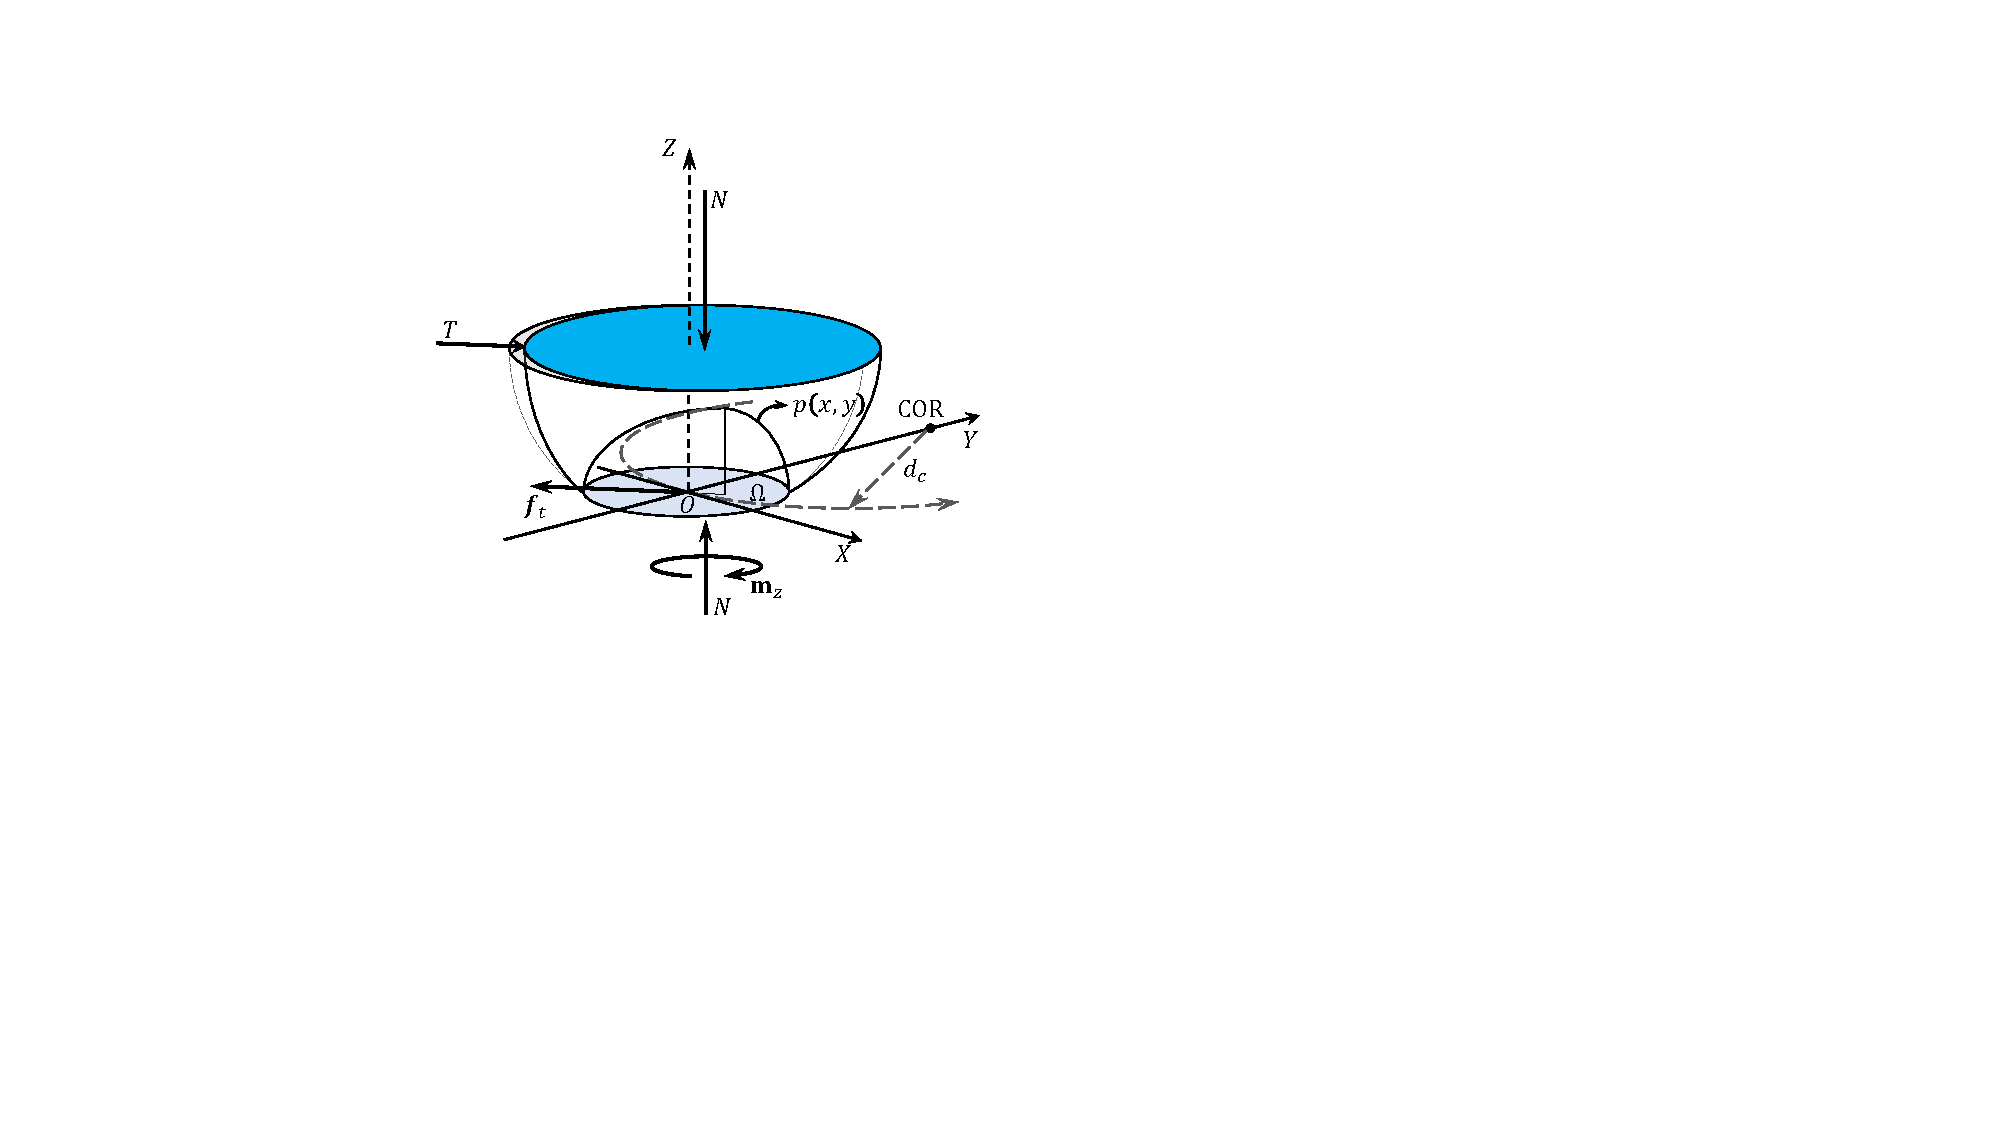
\includegraphics[scale=1]{Figures/SampleFigure.pdf}
\caption{شکل نمونه}
\label{Fig:SampleFigure1_2}
\end{figure}

نمونه‌ای از قرار دادن دو شکل در کنار یکدیگر در شکل
\ref{Fig:SampleFigure2_2}
آورده شده است.

\begin{figure}[!htb]
\centering
\subfloat[زیرنویس شکل اول]{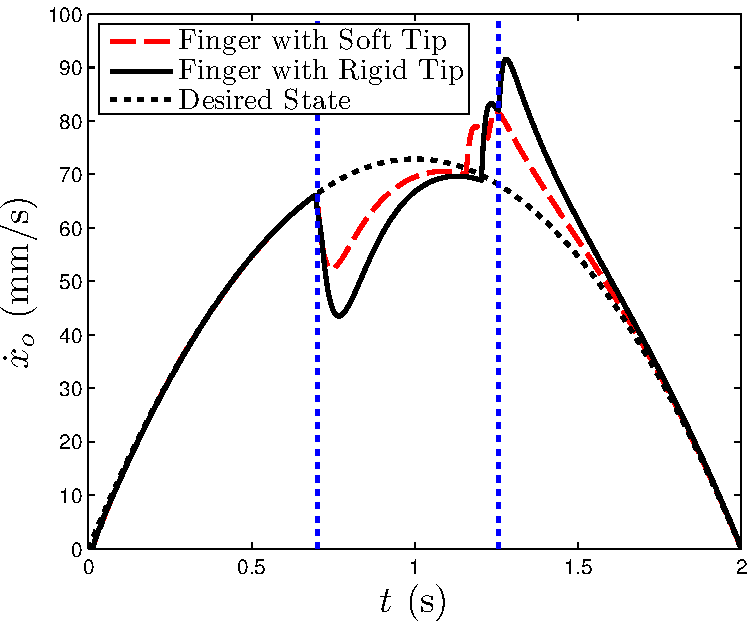
\includegraphics[scale=0.56]{Figures/FigureA.pdf}}
\quad
\subfloat[زیرنویس شکل دوم]{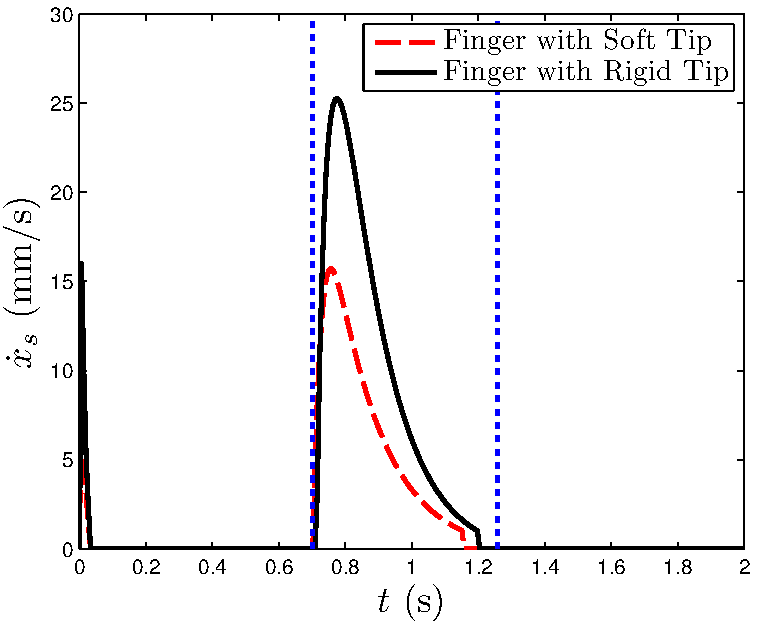
\includegraphics[scale=0.56]{Figures/FigureB.pdf}}
\caption{
قرار دادن دو شکل در کنار یکدیگر، الف) شکل نمونه اول،
ب) شکل نمونه دوم
}
\label{Fig:SampleFigure2_2}
\end{figure}





آیتم‌های مختلف به‌صورت زیر آورده می‌شود:
\begin{itemize}[label=-]
\item
مورد اول
\item
مورد دوم
\item
مورد سوم
\end{itemize}

نمونه‌ای از آیتم‌های شماره‌دار نیز در ادامه آورده شده است. به طور کلی معماری برداشت انرژی به دو دسته‌ی کلی تقسیم می‌شود:
\begin{enumerate}[label=\arabic*)]
\item
برداشت-استفاده:

در این حالت سیستم بلافاصله انرژی برداشت‌شده را مصرف می‌کند. واضح است اگر انرژی کافی در محیط وجود نداشته باشد دستگاه از کار می‌افتد. این نوع سیستم‌ها بیشتر در فشار دادن کلید‌ها، پدال‌ها و دستگاه‌های ردیابی برای انسان‌ها استفاده می‌شود. به طور مثال در پاشنه‌ی کفش دونده‌ای مواد پیزوالکتریک کار گذاشته می‌شود و با فشار پا بر روی کفش و فشرده شدن پیزوالکتریک داخل کفش، انرژی الکتریکی برای ارسال سیگنال 
\lr{RF}
و در نتیجه ردیابی دونده تامین می‌شود. 
\item
برداشت-ذخیره-استفاده:

در این روش سیستم برای ذخیره‌ی انرژی برداشت‌شده به باتری مجهز شده است. این روش برای زمانی‌که انرژی زیادی در محیط وجود داشته باشد و برای منابعی مانند انرژی خورشیدی  کاربرد دارد. روش‌های زیادی برای تبدیل انرژی خورشیدی به انرژی الکتریکی از جمله سلول‌های خورشیدی وجود دارد. در این حالت چگونگی ذخیره‌ی انرژی و بهینه‌سازی مصرف انرژی مطرح می‌شود.
\end{enumerate}




\subsection{زیربخش اول}
نوشته نمونه نوشته نمونه نوشته نمونه نوشته نمونه نوشته نمونه نوشته نمونه نوشته نمونه نوشته نمونه نوشته نمونه نوشته نمونه نوشته نمونه نوشته نمونه نوشته نمونه نوشته نمونه نوشته نمونه نوشته نمونه نوشته نمونه نوشته نمونه نوشته نمونه نوشته نمونه نوشته نمونه نوشته نمونه. در جدول
\ref{Tbl:SampleTable1_2}،
نمونه‌ای از یک جدول واردشده در لاتک و در جدول
\ref{Tbl:SampleTable2_2}،
نمونه‌ای از یک جدول نوشته‌شده در لاتک آورده شده است.

\begin{table}[!htb]
\caption{پارامترهای شبیه‌سازی}
\centering
\begin{tabular}{c}
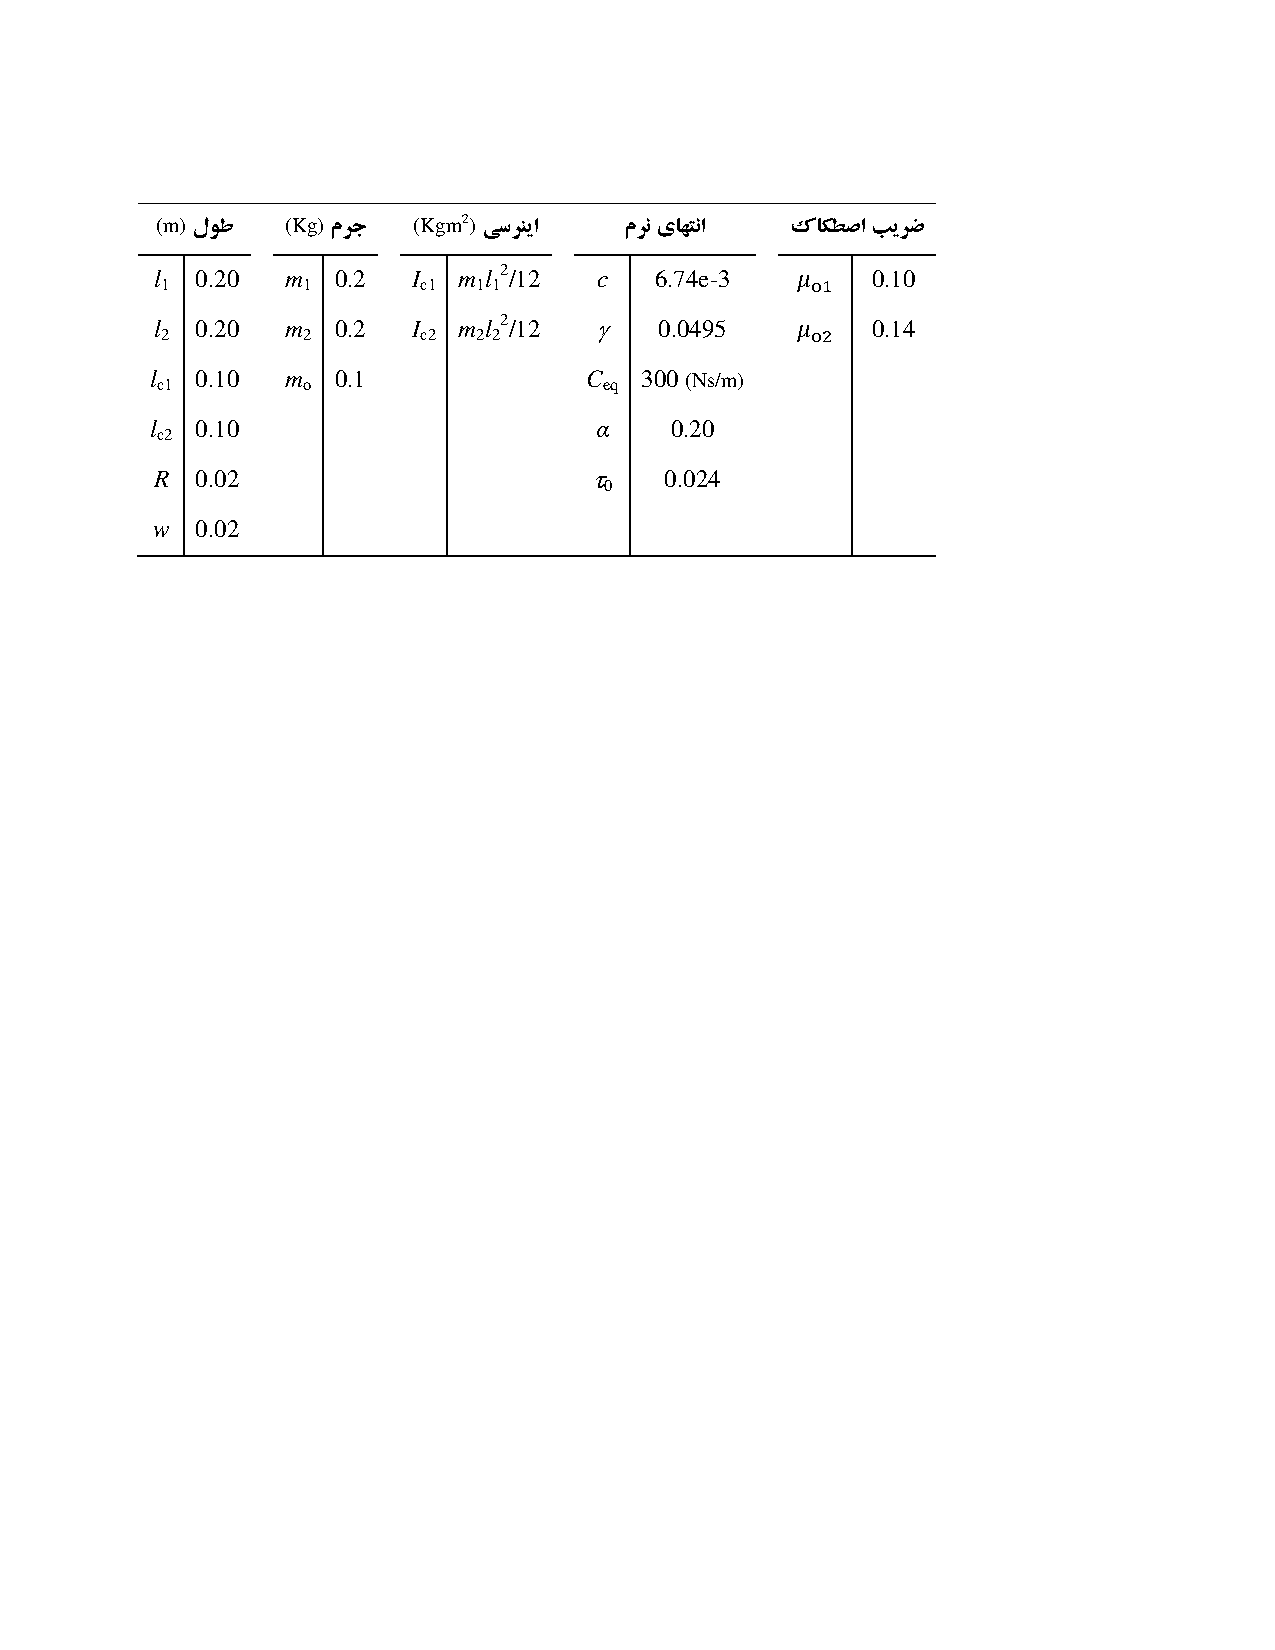
\includegraphics[scale=0.9]{Figures/SampleTable1.pdf} 
\end{tabular}
\vspace{-\baselineskip}
\label{Tbl:SampleTable1_2}
\end{table}

\begin{table}[!htb]
\caption{مقايسه‌ی روش‌هاي برداشت انرژي مبتني بر لرزش‌هاي مکانيکی}
\centering
\begin{tabular}{@{}|p{.15\textwidth}|p{.25\textwidth}|p{.25\textwidth}|p{.25\textwidth}|@{}}
\hline
روش
& 
چگالی انرژی
& 
ابعاد
& 
عیب اصلی
\\ \hline \hline
پیزوالکتریک
& 
$\mathrm{mJ/cm^3}$ 35/4
& 
بزرگ
& 
ولتاژ خروجی کم
\\ \hline
الکترومغناطیس
& 
$\mathrm{mJ/cm^3}$ 24/8
& 
بزرگ
& 
ولتاژ خروجی بسیار کم
\\ \hline
الکترواستاتیک
& 
$\mathrm{mJ/cm^3}$ 4
& 
فشرده در تراشه‌ها
& 
نیاز به منبع شارژ اولیه
\\ \hline
\end{tabular}
\label{Tbl:SampleTable2_2}
\vspace{-\baselineskip}
\end{table}

نمونه‌ای از یک رابطه به‌صورت
\begin{equation}
p\left( r \right) = {C_k}\frac{N}{{\pi {a^2}}}{\left[{1 - {{\left( {\frac{r}{a}} \right)}^k}} \right]^{\frac{1}{k}}},
\label{Eq:Pressure_2}
\end{equation}
است. در رابطه
\ref{Eq:Pressure_2}،
$N$
نیروی عمودی است. نمونه‌ای از استفاده از روابط متوالی به‌صورت
\begin{equation}
\sum \limits_{i = 1}^{k + 1} {E_s}\left( i \right) - T \sum \limits_{i = 1}^k {P_s}\left( i \right) \le B_s^{max},\quad k = 1, \ldots ,N - 1,
\label{Eq:batterysource_2}
\end{equation}\vspace{-\baselineskip}
\begin{equation}
\sum \limits_{i = 1}^{k + 1} {E_r}\left( i \right) - T \sum \limits_{i = 1}^k {P_r}\left( i \right) \le B_r^{max},\quad k = 1, \ldots ,N - 1,
\label{Eq:batteryrellay_2}
\end{equation}
است. نمونه‌ای از یک قضیه و تبصره نیز در ادامه آورده شده است.
\begin{theorem}
اگر ظرفیت باتری‌ها به اندازه کافی بزرگ باشد، جواب بهینه‌ی 
$P_s^*(i)$
و
$P_r^*(i)$
وجود دارد به نحوی که تابع هدف را بیشینه می‌کند و در رابطه‌ی زیر صدق می‌کند:
\begin{equation}
C\left( {{{\left| {{h_{sr}}\left( i \right)} \right|}^2}{P_s}^*\left( i \right)} \right) \ge C\left( {{{\left| {{h_{sd}}\left( i \right)} \right|}^2}{P_s}^*\left( i \right)} \right) + C\left( {{{\left| {{h_{rd}}\left( {i + 1} \right)} \right|}^2}P_r^*\left( {i} \right)} \right).
\label{Eq:theorem1_2}
\end{equation}

\begin{proof}
بار دیگر فرم تابع هدف را در نظر می‌گیریم. لازم به ذکر است اینجا تابع هدف یک تابع دومتغیره است.
\begin{equation}
{R({\mathbf{P}_s},{\mathbf{P}_r}) = {\frac{1}{2}\sum\limits_{i = 1}^N {\min } \left\{ {C\left( {{{\left| {{h_{sr}}\left( i \right)} \right|}^2}{P_s}\left( i \right)} \right),} C\left( {{{\left| {{h_{sd}}\left( i \right)} \right|}^2}{P_s}\left( i \right)} \right) \right\} }}.
\end{equation}
حال بلوک
$i$ام
را در نظر می‌گیریم. اگر رابطه‌ی
\ref{Eq:theorem1_2}
برای
$i$
برقرار نباشد، به عبارت دیگر اگر داشته باشیم،
\begin{equation}
C\left( {{{\left| {{h_{sr}}\left( i \right)} \right|}^2}{P_s}^*\left( i \right)} \right) < C\left( {{{\left| {{h_{sd}}\left( i \right)} \right|}^2}{P_s}^*\left( i \right)} \right) + C\left( {{{\left| {{h_{rd}}\left( {i + 1} \right)} \right|}^2}P_r^*\left( {i + 1} \right)} \right),
\label{Eq:theorem1(2)_2}
\end{equation}
بنابراین
\begin{equation}
C\left( {{{\left| {{h_{sr}}\left( i \right)} \right|}^2}{P_s}^*\left( i \right)} \right)+ C\left( {{{\left| {{h_{sd}}\left( i \right)} \right|}^2}{P_s}^*\left( i \right)} \right) =C\left( {{{\left| {{h_{sr}}\left( i \right)} \right|}^2}{P_s}^*\left( i \right)} \right).
\end{equation}
پس در تابع هدف مسئله، مقدار بهینه‌ی مسئله برابر عبارت سمت چپ رابطه‌ی
\ref{Eq:theorem1(2)_2}
شده است و آرگومان دوم و  هم‌چنین مقدار
$P_r^*(i)$
هیچ نقشی در مقدار بهینه ندارد. بنابراین می‌توانیم 
$P_r^*(i)$
را آنقدر کاهش دهیم تا در رابطه‌ی
\ref{Eq:theorem1(2)_2}
تساوی برقرار شود بدون آنکه مقدار بهینه‌ی مسئله تغییر کند.
\end{proof}
\label{theorem1_2}
\end{theorem}

\begin{remark}
از قضیه‌ی
\ref{theorem1_2}
نتیجه می‌گیریم که جواب بهینه‌ی مسئله‌ی
\lr{P}
در حالت کلی یکتا نیست. به طور مثال وقتی مقدار انرژی برداشت‌شده در رله خیلی بیشتر از این انرژی در منبع باشد مسئله می‌تواند جواب‌های زیادی داشته باشد. بنابراین همواره می‌توان برای صرفه‌جویی در مصرف انرژی، بدون کاهش مقدار نرخ گذردهی سیستم، کمترین مقدار توان را برای رله انتخاب کرد. بنابراین با توجه به رابطه
\begin{equation}
C\left( {{{\left| {{h_{sr}}\left( i \right)} \right|}^2}{P_s}^*\left( i \right)} \right) 
\ge C\left( {{{\left| {{h_{sd}}\left( i \right)} \right|}^2}{P_s}^*\left( i \right)} \right) + C\left( {{{\left| {{h_{rd}}\left( {i} \right)} \right|}^2}P_r^*\left( {i} \right)} \right),
\label{Eq:remark1_2}
\end{equation}
و با  استفاده از رابطه
\ref{Eq:remark1_2}
خواهیم داشت،
\begin{equation}
{R_r}(i) = \min \left\{ {C\left( {{{\left| {{h_{rd}}(i)} \right|}^2}{P_r}(i)} \right),C\left( {{{\left| {{h_{sr}}(i)} \right|}^2}{P_s}(i)} \right)} \right\}.
\end{equation}

بنابراین می‌توان با انتخاب کمترین توان و نرخ برای رله از مصرف بی‌رویه‌ی انرژی جلوگیری کرد. فرض بزرگ بودن ظرفیت باتری‌ به این دلیل است که اگر ظرفیت باتری محدود باشد برای کاهش
$P_r^*(i)$
با محدودیت مواجه هستیم. چون در صورت کاهش بی از حد توان رله ممکن است از ناحیه‌ی شدنی مسئله خارج شویم. به هر حال برای هر دو حالت ظرفیت نامحدود و محدود باتری جواب مسئله یکتا نیست و همواره می‌توان با کاهش توان رله مصرف انرژی را کاهش داد.
\end{remark}




\section{پیش‌گفتار}
در این قالب سعی شده است که از تمامی بخش‌های موجود در پایان‌نامه‌ها نمونه‌ای آورده شود. در این قالب سعی شده است که از تمامی بخش‌های موجود در پایان‌نامه‌ها نمونه‌ای آورده شود. در این قالب سعی شده است که از تمامی بخش‌های موجود در پایان‌نامه‌ها نمونه‌ای آورده شود. در این قالب سعی شده است که از تمامی بخش‌های موجود در پایان‌نامه‌ها نمونه‌ای آورده شود. در این قالب سعی شده است که از تمامی بخش‌های موجود در پایان‌نامه‌ها نمونه‌ای آورده شود. در این قالب سعی شده است که از تمامی بخش‌های موجود در پایان‌نامه‌ها نمونه‌ای آورده شود. در این قالب سعی شده است که از تمامی بخش‌های موجود در پایان‌نامه‌ها نمونه‌ای آورده شود. در این قالب سعی شده است که از تمامی بخش‌های موجود در پایان‌نامه‌ها نمونه‌ای آورده شود. در این قالب سعی شده است که از تمامی بخش‌های موجود در پایان‌نامه‌ها نمونه‌ای آورده شود. در این قالب سعی شده است که از تمامی بخش‌های موجود در پایان‌نامه‌ها نمونه‌ای آورده شود. در این قالب سعی شده است که از تمامی بخش‌های موجود در پایان‌نامه‌ها نمونه‌ای آورده شود. در این قالب سعی شده است که از تمامی بخش‌های موجود در پایان‌نامه‌ها نمونه‌ای آورده شود. در این قالب سعی شده است که از تمامی بخش‌های موجود در پایان‌نامه‌ها نمونه‌ای آورده شود. در این قالب سعی شده است که از تمامی بخش‌های موجود در پایان‌نامه‌ها نمونه‌ای آورده شود.
\section{بخش اول}
نمونه‌ای از یک عبارت انگلیسی در متن به‌صورت
\lr{English Sentence}
است. نمونه‌ای از یک عبارت ریاضی در متن نیز به‌صورت
$x^2 + y^2$
است. ارجاع به مراجع انگلیسی
\cite{Fakhari2015a,Lewis2003}.
ارجاع به مراجع فارسی
\cite{Fakhari2015b,HadianThesis2008}.
این نمونه‌ای از یک زیرنویس انگلیسی%
\LTRfootnote{English Footnote}
است. این نمونه‌ای از یک زیرنویس فارسی%
\RTLfootnote{زیرنویس فارسی}
است. در شکل
\ref{Fig:SampleFigure1_2}،
نمونه‌ای از یک شکل آورده شده است. 

\begin{figure}[!htb]
\centering
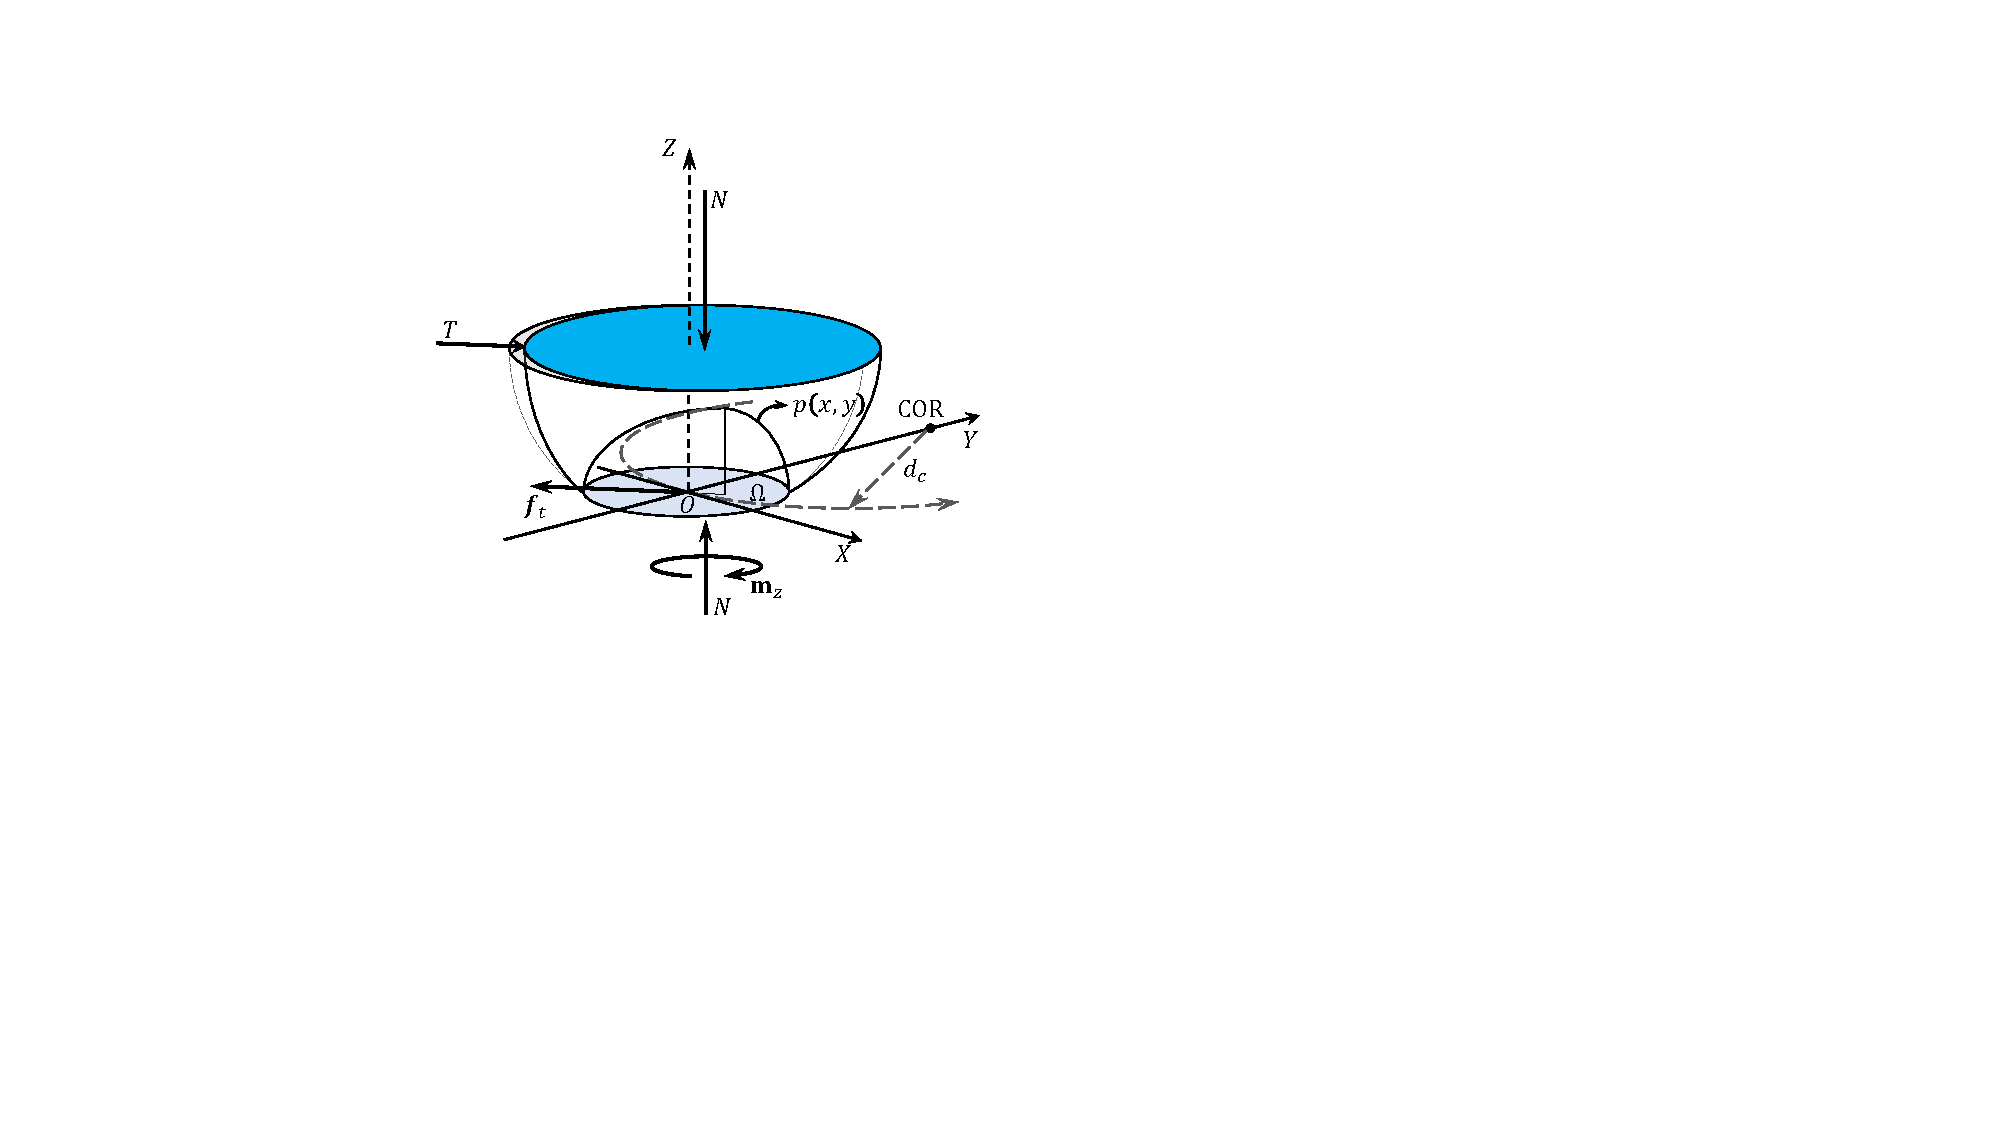
\includegraphics[scale=1]{Figures/SampleFigure.pdf}
\caption{شکل نمونه}
\label{Fig:SampleFigure1_2}
\end{figure}

نمونه‌ای از قرار دادن دو شکل در کنار یکدیگر در شکل
\ref{Fig:SampleFigure2_2}
آورده شده است.

\begin{figure}[!htb]
\centering
\subfloat[زیرنویس شکل اول]{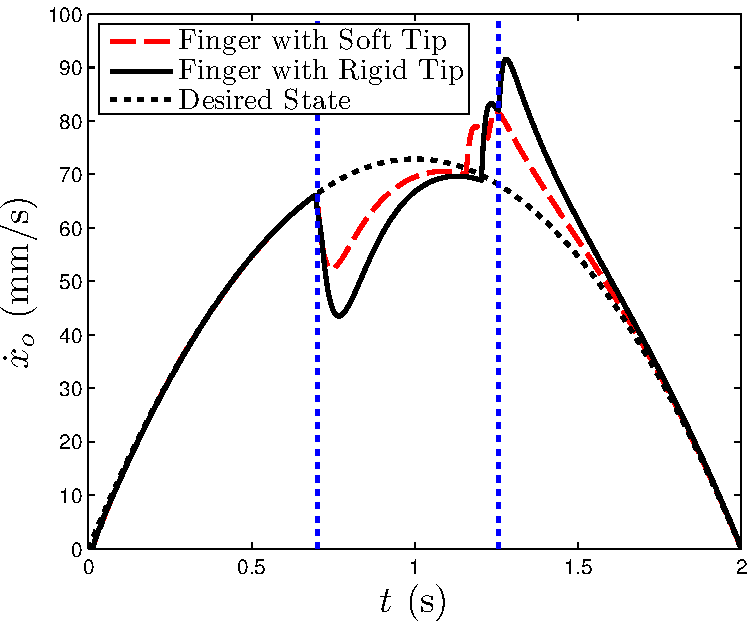
\includegraphics[scale=0.56]{Figures/FigureA.pdf}}
\quad
\subfloat[زیرنویس شکل دوم]{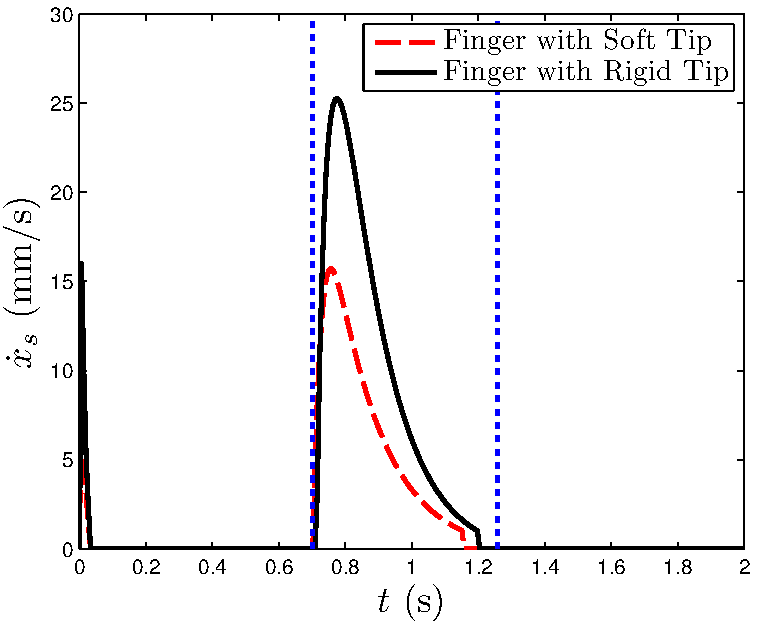
\includegraphics[scale=0.56]{Figures/FigureB.pdf}}
\caption{
قرار دادن دو شکل در کنار یکدیگر، الف) شکل نمونه اول،
ب) شکل نمونه دوم
}
\label{Fig:SampleFigure2_2}
\end{figure}





آیتم‌های مختلف به‌صورت زیر آورده می‌شود:
\begin{itemize}[label=-]
\item
مورد اول
\item
مورد دوم
\item
مورد سوم
\end{itemize}

نمونه‌ای از آیتم‌های شماره‌دار نیز در ادامه آورده شده است. به طور کلی معماری برداشت انرژی به دو دسته‌ی کلی تقسیم می‌شود:
\begin{enumerate}[label=\arabic*)]
\item
برداشت-استفاده:

در این حالت سیستم بلافاصله انرژی برداشت‌شده را مصرف می‌کند. واضح است اگر انرژی کافی در محیط وجود نداشته باشد دستگاه از کار می‌افتد. این نوع سیستم‌ها بیشتر در فشار دادن کلید‌ها، پدال‌ها و دستگاه‌های ردیابی برای انسان‌ها استفاده می‌شود. به طور مثال در پاشنه‌ی کفش دونده‌ای مواد پیزوالکتریک کار گذاشته می‌شود و با فشار پا بر روی کفش و فشرده شدن پیزوالکتریک داخل کفش، انرژی الکتریکی برای ارسال سیگنال 
\lr{RF}
و در نتیجه ردیابی دونده تامین می‌شود. 
\item
برداشت-ذخیره-استفاده:

در این روش سیستم برای ذخیره‌ی انرژی برداشت‌شده به باتری مجهز شده است. این روش برای زمانی‌که انرژی زیادی در محیط وجود داشته باشد و برای منابعی مانند انرژی خورشیدی  کاربرد دارد. روش‌های زیادی برای تبدیل انرژی خورشیدی به انرژی الکتریکی از جمله سلول‌های خورشیدی وجود دارد. در این حالت چگونگی ذخیره‌ی انرژی و بهینه‌سازی مصرف انرژی مطرح می‌شود.
\end{enumerate}




\subsection{زیربخش اول}
نوشته نمونه نوشته نمونه نوشته نمونه نوشته نمونه نوشته نمونه نوشته نمونه نوشته نمونه نوشته نمونه نوشته نمونه نوشته نمونه نوشته نمونه نوشته نمونه نوشته نمونه نوشته نمونه نوشته نمونه نوشته نمونه نوشته نمونه نوشته نمونه نوشته نمونه نوشته نمونه نوشته نمونه نوشته نمونه. در جدول
\ref{Tbl:SampleTable1_2}،
نمونه‌ای از یک جدول واردشده در لاتک و در جدول
\ref{Tbl:SampleTable2_2}،
نمونه‌ای از یک جدول نوشته‌شده در لاتک آورده شده است.

\begin{table}[!htb]
\caption{پارامترهای شبیه‌سازی}
\centering
\begin{tabular}{c}
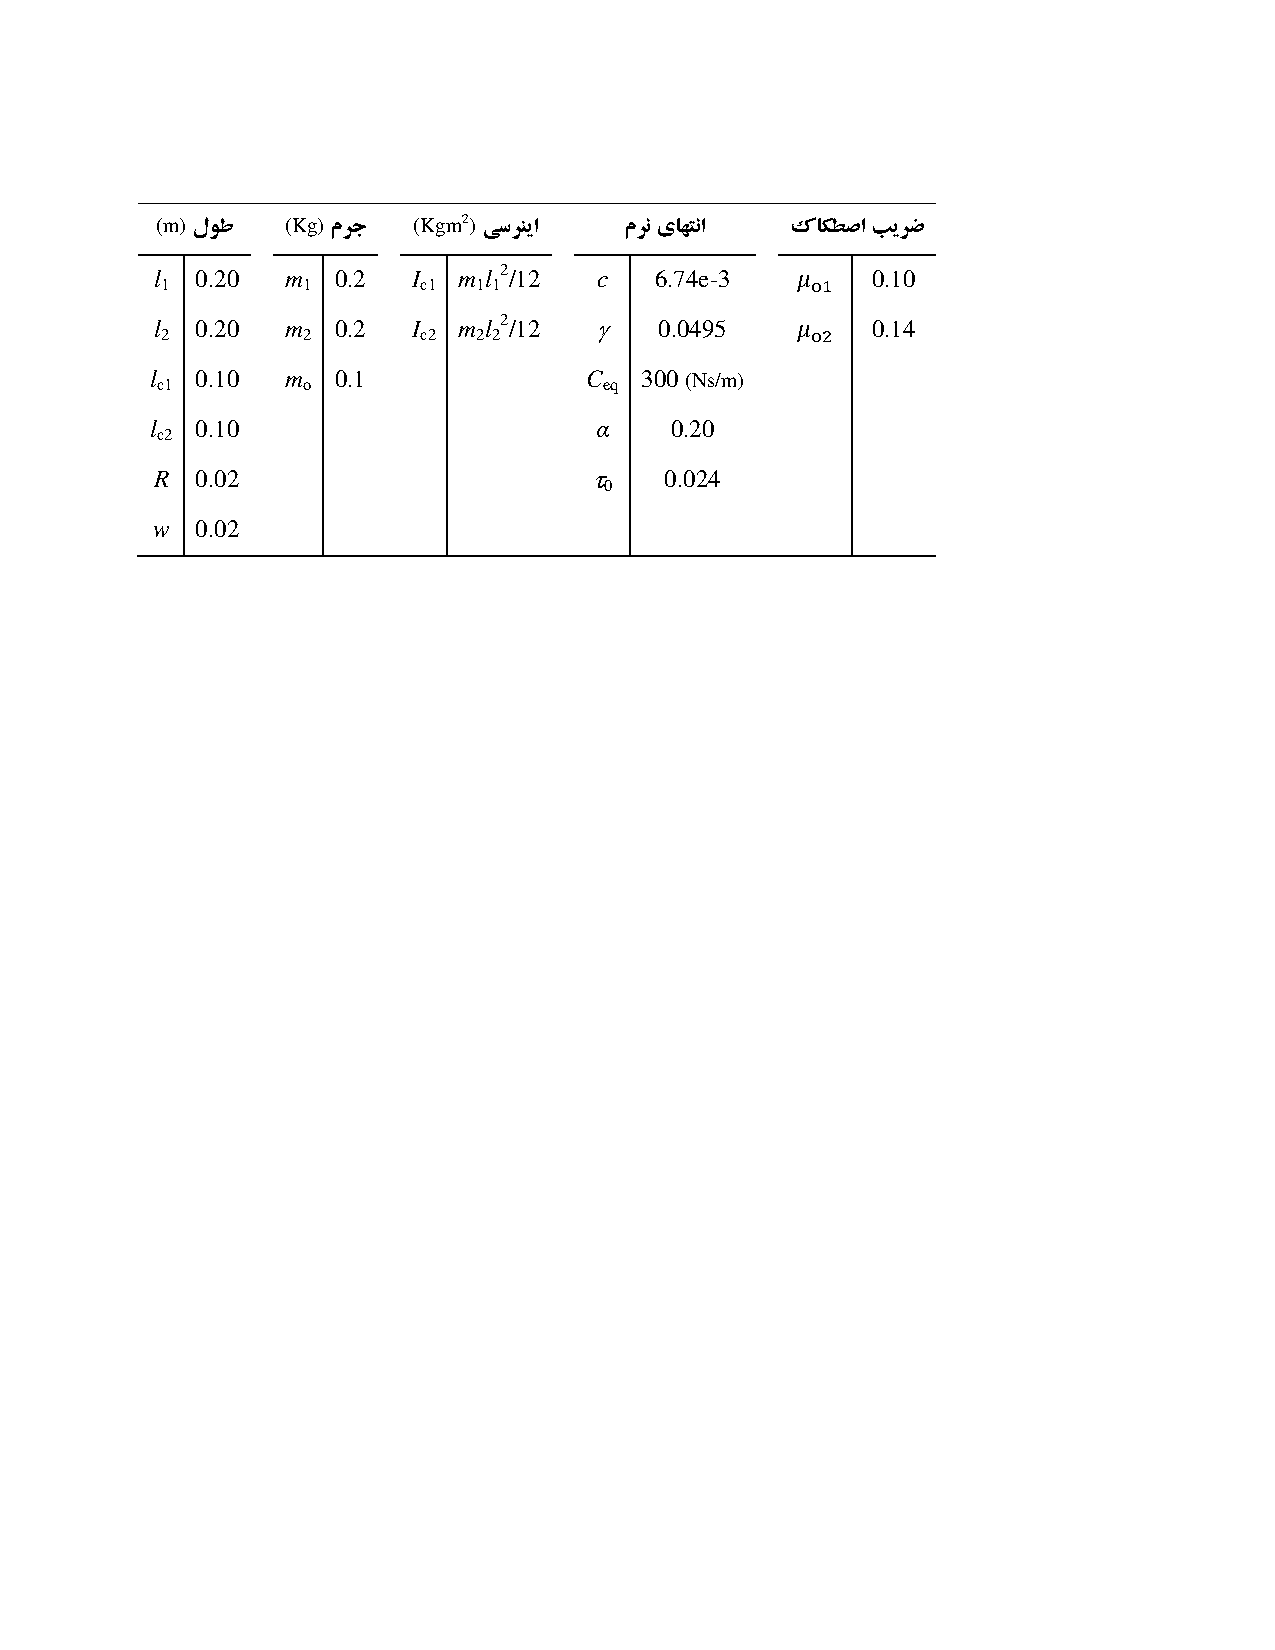
\includegraphics[scale=0.9]{Figures/SampleTable1.pdf} 
\end{tabular}
\vspace{-\baselineskip}
\label{Tbl:SampleTable1_2}
\end{table}

\begin{table}[!htb]
\caption{مقايسه‌ی روش‌هاي برداشت انرژي مبتني بر لرزش‌هاي مکانيکی}
\centering
\begin{tabular}{@{}|p{.15\textwidth}|p{.25\textwidth}|p{.25\textwidth}|p{.25\textwidth}|@{}}
\hline
روش
& 
چگالی انرژی
& 
ابعاد
& 
عیب اصلی
\\ \hline \hline
پیزوالکتریک
& 
$\mathrm{mJ/cm^3}$ 35/4
& 
بزرگ
& 
ولتاژ خروجی کم
\\ \hline
الکترومغناطیس
& 
$\mathrm{mJ/cm^3}$ 24/8
& 
بزرگ
& 
ولتاژ خروجی بسیار کم
\\ \hline
الکترواستاتیک
& 
$\mathrm{mJ/cm^3}$ 4
& 
فشرده در تراشه‌ها
& 
نیاز به منبع شارژ اولیه
\\ \hline
\end{tabular}
\label{Tbl:SampleTable2_2}
\vspace{-\baselineskip}
\end{table}

نمونه‌ای از یک رابطه به‌صورت
\begin{equation}
p\left( r \right) = {C_k}\frac{N}{{\pi {a^2}}}{\left[{1 - {{\left( {\frac{r}{a}} \right)}^k}} \right]^{\frac{1}{k}}},
\label{Eq:Pressure_2}
\end{equation}
است. در رابطه
\ref{Eq:Pressure_2}،
$N$
نیروی عمودی است. نمونه‌ای از استفاده از روابط متوالی به‌صورت
\begin{equation}
\sum \limits_{i = 1}^{k + 1} {E_s}\left( i \right) - T \sum \limits_{i = 1}^k {P_s}\left( i \right) \le B_s^{max},\quad k = 1, \ldots ,N - 1,
\label{Eq:batterysource_2}
\end{equation}\vspace{-\baselineskip}
\begin{equation}
\sum \limits_{i = 1}^{k + 1} {E_r}\left( i \right) - T \sum \limits_{i = 1}^k {P_r}\left( i \right) \le B_r^{max},\quad k = 1, \ldots ,N - 1,
\label{Eq:batteryrellay_2}
\end{equation}
است. نمونه‌ای از یک قضیه و تبصره نیز در ادامه آورده شده است.
\begin{theorem}
اگر ظرفیت باتری‌ها به اندازه کافی بزرگ باشد، جواب بهینه‌ی 
$P_s^*(i)$
و
$P_r^*(i)$
وجود دارد به نحوی که تابع هدف را بیشینه می‌کند و در رابطه‌ی زیر صدق می‌کند:
\begin{equation}
C\left( {{{\left| {{h_{sr}}\left( i \right)} \right|}^2}{P_s}^*\left( i \right)} \right) \ge C\left( {{{\left| {{h_{sd}}\left( i \right)} \right|}^2}{P_s}^*\left( i \right)} \right) + C\left( {{{\left| {{h_{rd}}\left( {i + 1} \right)} \right|}^2}P_r^*\left( {i} \right)} \right).
\label{Eq:theorem1_2}
\end{equation}

\begin{proof}
بار دیگر فرم تابع هدف را در نظر می‌گیریم. لازم به ذکر است اینجا تابع هدف یک تابع دومتغیره است.
\begin{equation}
{R({\mathbf{P}_s},{\mathbf{P}_r}) = {\frac{1}{2}\sum\limits_{i = 1}^N {\min } \left\{ {C\left( {{{\left| {{h_{sr}}\left( i \right)} \right|}^2}{P_s}\left( i \right)} \right),} C\left( {{{\left| {{h_{sd}}\left( i \right)} \right|}^2}{P_s}\left( i \right)} \right) \right\} }}.
\end{equation}
حال بلوک
$i$ام
را در نظر می‌گیریم. اگر رابطه‌ی
\ref{Eq:theorem1_2}
برای
$i$
برقرار نباشد، به عبارت دیگر اگر داشته باشیم،
\begin{equation}
C\left( {{{\left| {{h_{sr}}\left( i \right)} \right|}^2}{P_s}^*\left( i \right)} \right) < C\left( {{{\left| {{h_{sd}}\left( i \right)} \right|}^2}{P_s}^*\left( i \right)} \right) + C\left( {{{\left| {{h_{rd}}\left( {i + 1} \right)} \right|}^2}P_r^*\left( {i + 1} \right)} \right),
\label{Eq:theorem1(2)_2}
\end{equation}
بنابراین
\begin{equation}
C\left( {{{\left| {{h_{sr}}\left( i \right)} \right|}^2}{P_s}^*\left( i \right)} \right)+ C\left( {{{\left| {{h_{sd}}\left( i \right)} \right|}^2}{P_s}^*\left( i \right)} \right) =C\left( {{{\left| {{h_{sr}}\left( i \right)} \right|}^2}{P_s}^*\left( i \right)} \right).
\end{equation}
پس در تابع هدف مسئله، مقدار بهینه‌ی مسئله برابر عبارت سمت چپ رابطه‌ی
\ref{Eq:theorem1(2)_2}
شده است و آرگومان دوم و  هم‌چنین مقدار
$P_r^*(i)$
هیچ نقشی در مقدار بهینه ندارد. بنابراین می‌توانیم 
$P_r^*(i)$
را آنقدر کاهش دهیم تا در رابطه‌ی
\ref{Eq:theorem1(2)_2}
تساوی برقرار شود بدون آنکه مقدار بهینه‌ی مسئله تغییر کند.
\end{proof}
\label{theorem1_2}
\end{theorem}

\begin{remark}
از قضیه‌ی
\ref{theorem1_2}
نتیجه می‌گیریم که جواب بهینه‌ی مسئله‌ی
\lr{P}
در حالت کلی یکتا نیست. به طور مثال وقتی مقدار انرژی برداشت‌شده در رله خیلی بیشتر از این انرژی در منبع باشد مسئله می‌تواند جواب‌های زیادی داشته باشد. بنابراین همواره می‌توان برای صرفه‌جویی در مصرف انرژی، بدون کاهش مقدار نرخ گذردهی سیستم، کمترین مقدار توان را برای رله انتخاب کرد. بنابراین با توجه به رابطه
\begin{equation}
C\left( {{{\left| {{h_{sr}}\left( i \right)} \right|}^2}{P_s}^*\left( i \right)} \right) 
\ge C\left( {{{\left| {{h_{sd}}\left( i \right)} \right|}^2}{P_s}^*\left( i \right)} \right) + C\left( {{{\left| {{h_{rd}}\left( {i} \right)} \right|}^2}P_r^*\left( {i} \right)} \right),
\label{Eq:remark1_2}
\end{equation}
و با  استفاده از رابطه
\ref{Eq:remark1_2}
خواهیم داشت،
\begin{equation}
{R_r}(i) = \min \left\{ {C\left( {{{\left| {{h_{rd}}(i)} \right|}^2}{P_r}(i)} \right),C\left( {{{\left| {{h_{sr}}(i)} \right|}^2}{P_s}(i)} \right)} \right\}.
\end{equation}

بنابراین می‌توان با انتخاب کمترین توان و نرخ برای رله از مصرف بی‌رویه‌ی انرژی جلوگیری کرد. فرض بزرگ بودن ظرفیت باتری‌ به این دلیل است که اگر ظرفیت باتری محدود باشد برای کاهش
$P_r^*(i)$
با محدودیت مواجه هستیم. چون در صورت کاهش بی از حد توان رله ممکن است از ناحیه‌ی شدنی مسئله خارج شویم. به هر حال برای هر دو حالت ظرفیت نامحدود و محدود باتری جواب مسئله یکتا نیست و همواره می‌توان با کاهش توان رله مصرف انرژی را کاهش داد.
\end{remark}




\section{پیش‌گفتار}
در این قالب سعی شده است که از تمامی بخش‌های موجود در پایان‌نامه‌ها نمونه‌ای آورده شود. در این قالب سعی شده است که از تمامی بخش‌های موجود در پایان‌نامه‌ها نمونه‌ای آورده شود. در این قالب سعی شده است که از تمامی بخش‌های موجود در پایان‌نامه‌ها نمونه‌ای آورده شود. در این قالب سعی شده است که از تمامی بخش‌های موجود در پایان‌نامه‌ها نمونه‌ای آورده شود. در این قالب سعی شده است که از تمامی بخش‌های موجود در پایان‌نامه‌ها نمونه‌ای آورده شود. در این قالب سعی شده است که از تمامی بخش‌های موجود در پایان‌نامه‌ها نمونه‌ای آورده شود. در این قالب سعی شده است که از تمامی بخش‌های موجود در پایان‌نامه‌ها نمونه‌ای آورده شود. در این قالب سعی شده است که از تمامی بخش‌های موجود در پایان‌نامه‌ها نمونه‌ای آورده شود. در این قالب سعی شده است که از تمامی بخش‌های موجود در پایان‌نامه‌ها نمونه‌ای آورده شود. در این قالب سعی شده است که از تمامی بخش‌های موجود در پایان‌نامه‌ها نمونه‌ای آورده شود. در این قالب سعی شده است که از تمامی بخش‌های موجود در پایان‌نامه‌ها نمونه‌ای آورده شود. در این قالب سعی شده است که از تمامی بخش‌های موجود در پایان‌نامه‌ها نمونه‌ای آورده شود. در این قالب سعی شده است که از تمامی بخش‌های موجود در پایان‌نامه‌ها نمونه‌ای آورده شود. در این قالب سعی شده است که از تمامی بخش‌های موجود در پایان‌نامه‌ها نمونه‌ای آورده شود.
\section{بخش اول}
نمونه‌ای از یک عبارت انگلیسی در متن به‌صورت
\lr{English Sentence}
است. نمونه‌ای از یک عبارت ریاضی در متن نیز به‌صورت
$x^2 + y^2$
است. ارجاع به مراجع انگلیسی
\cite{Fakhari2015a,Lewis2003}.
ارجاع به مراجع فارسی
\cite{Fakhari2015b,HadianThesis2008}.
این نمونه‌ای از یک زیرنویس انگلیسی%
\LTRfootnote{English Footnote}
است. این نمونه‌ای از یک زیرنویس فارسی%
\RTLfootnote{زیرنویس فارسی}
است. در شکل
\ref{Fig:SampleFigure1_2}،
نمونه‌ای از یک شکل آورده شده است. 

\begin{figure}[!htb]
\centering
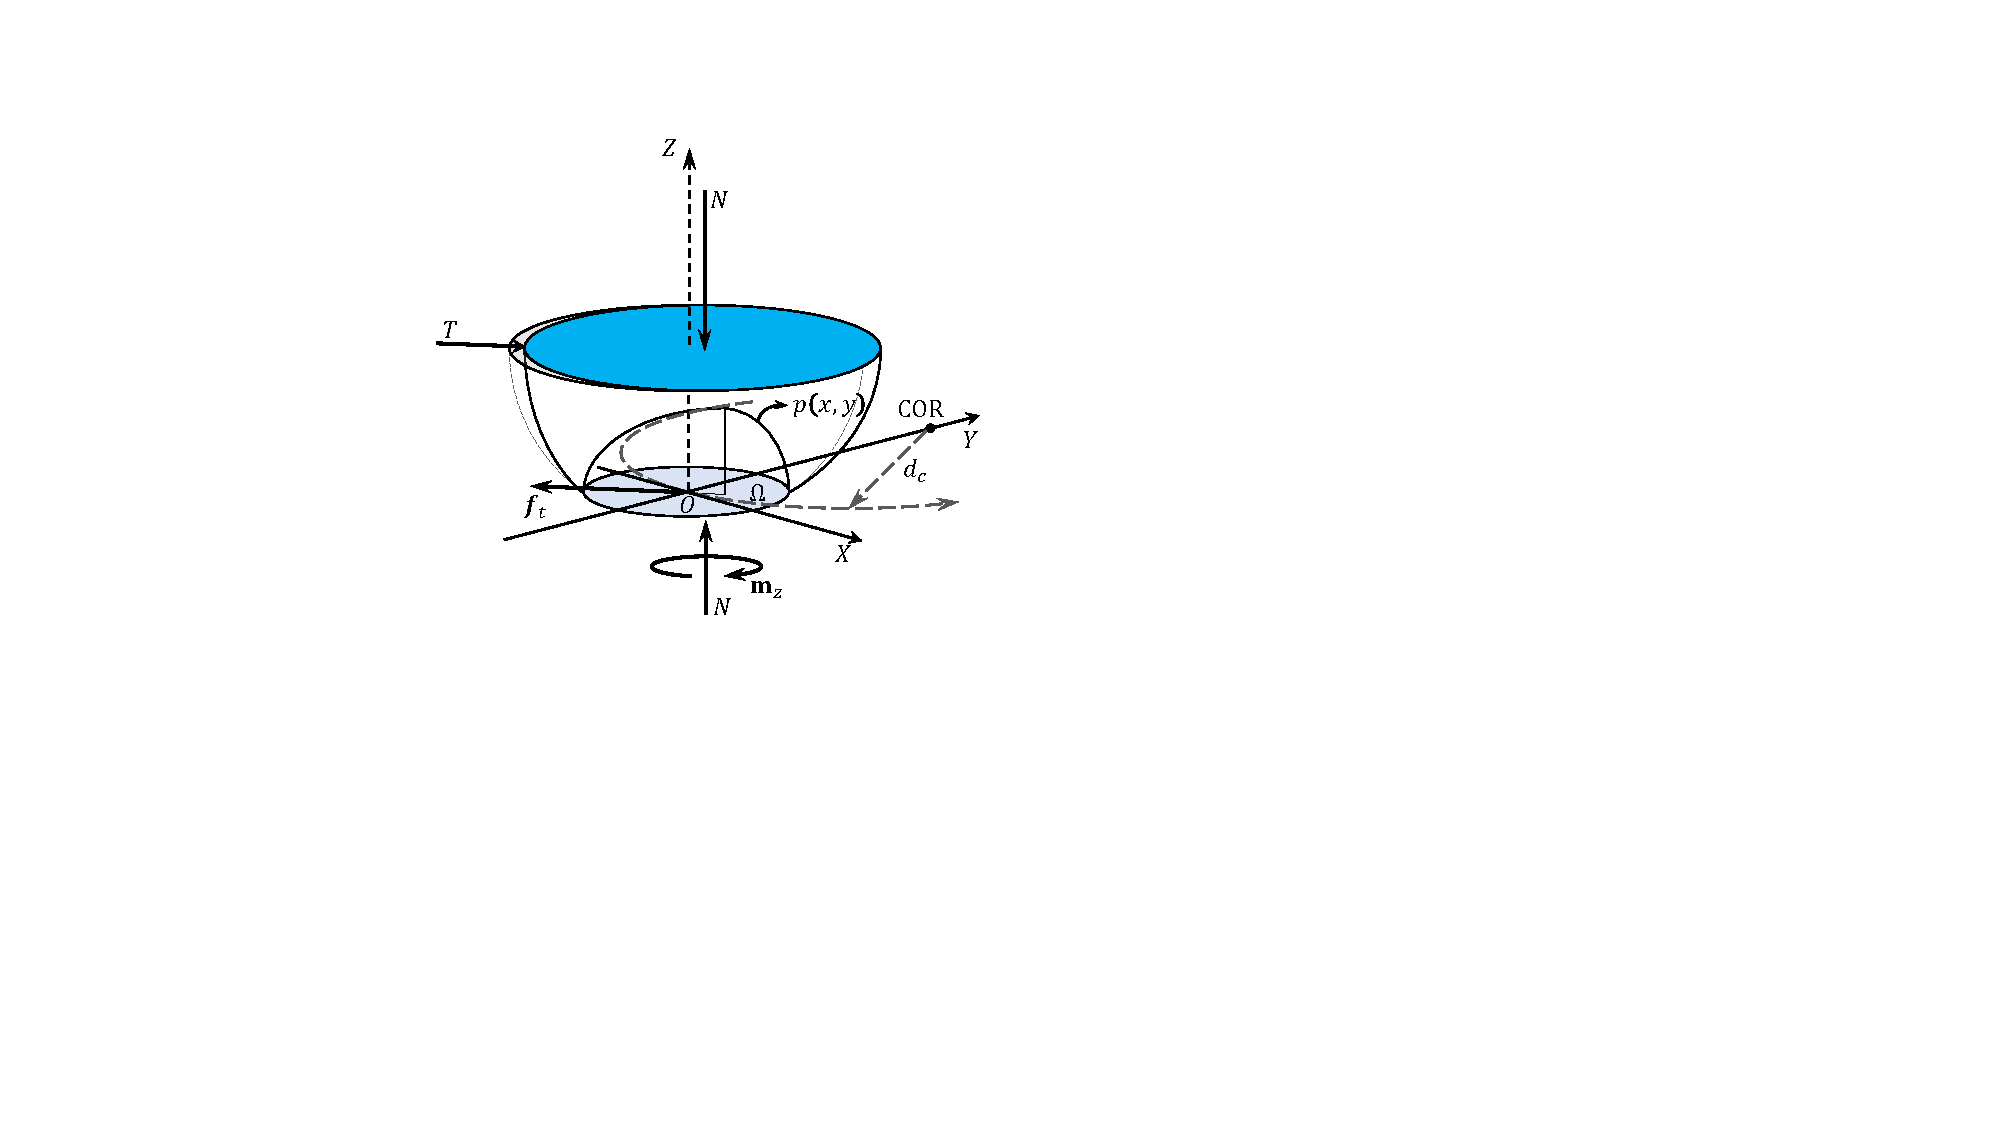
\includegraphics[scale=1]{Figures/SampleFigure.pdf}
\caption{شکل نمونه}
\label{Fig:SampleFigure1_2}
\end{figure}

نمونه‌ای از قرار دادن دو شکل در کنار یکدیگر در شکل
\ref{Fig:SampleFigure2_2}
آورده شده است.

\begin{figure}[!htb]
\centering
\subfloat[زیرنویس شکل اول]{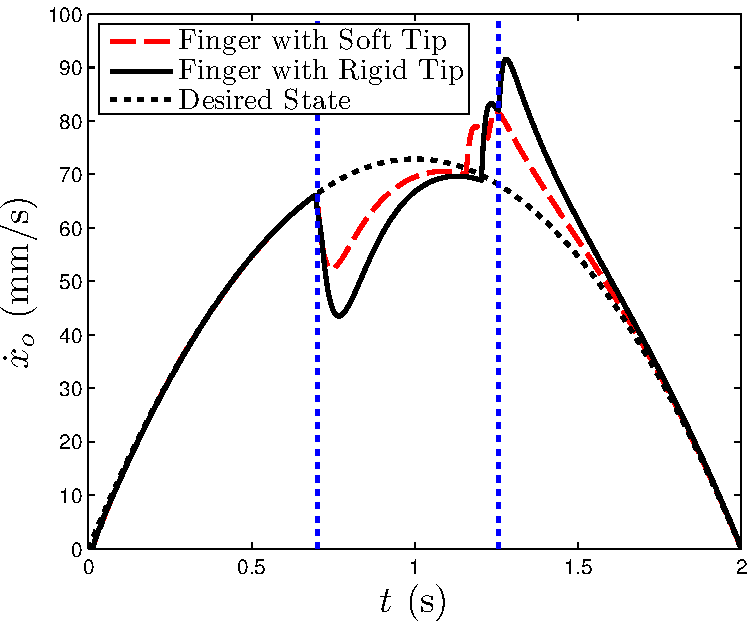
\includegraphics[scale=0.56]{Figures/FigureA.pdf}}
\quad
\subfloat[زیرنویس شکل دوم]{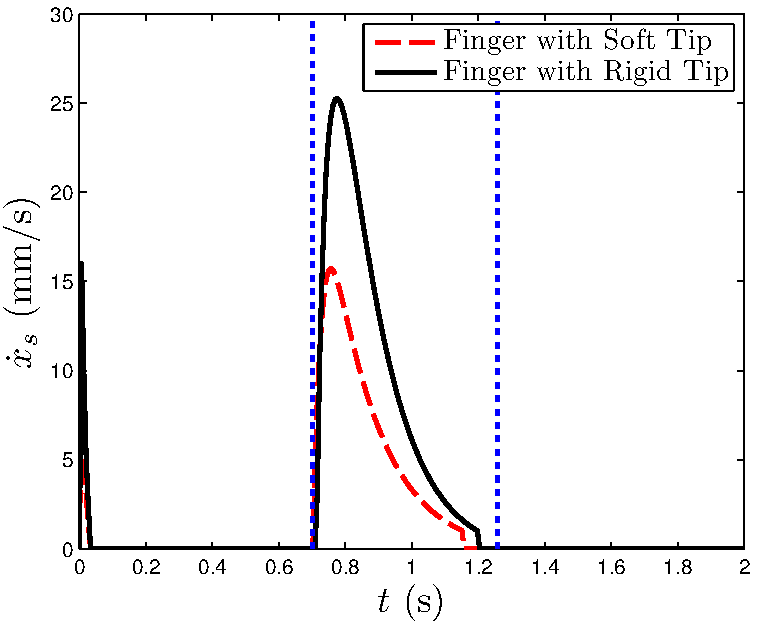
\includegraphics[scale=0.56]{Figures/FigureB.pdf}}
\caption{
قرار دادن دو شکل در کنار یکدیگر، الف) شکل نمونه اول،
ب) شکل نمونه دوم
}
\label{Fig:SampleFigure2_2}
\end{figure}





آیتم‌های مختلف به‌صورت زیر آورده می‌شود:
\begin{itemize}[label=-]
\item
مورد اول
\item
مورد دوم
\item
مورد سوم
\end{itemize}

نمونه‌ای از آیتم‌های شماره‌دار نیز در ادامه آورده شده است. به طور کلی معماری برداشت انرژی به دو دسته‌ی کلی تقسیم می‌شود:
\begin{enumerate}[label=\arabic*)]
\item
برداشت-استفاده:

در این حالت سیستم بلافاصله انرژی برداشت‌شده را مصرف می‌کند. واضح است اگر انرژی کافی در محیط وجود نداشته باشد دستگاه از کار می‌افتد. این نوع سیستم‌ها بیشتر در فشار دادن کلید‌ها، پدال‌ها و دستگاه‌های ردیابی برای انسان‌ها استفاده می‌شود. به طور مثال در پاشنه‌ی کفش دونده‌ای مواد پیزوالکتریک کار گذاشته می‌شود و با فشار پا بر روی کفش و فشرده شدن پیزوالکتریک داخل کفش، انرژی الکتریکی برای ارسال سیگنال 
\lr{RF}
و در نتیجه ردیابی دونده تامین می‌شود. 
\item
برداشت-ذخیره-استفاده:

در این روش سیستم برای ذخیره‌ی انرژی برداشت‌شده به باتری مجهز شده است. این روش برای زمانی‌که انرژی زیادی در محیط وجود داشته باشد و برای منابعی مانند انرژی خورشیدی  کاربرد دارد. روش‌های زیادی برای تبدیل انرژی خورشیدی به انرژی الکتریکی از جمله سلول‌های خورشیدی وجود دارد. در این حالت چگونگی ذخیره‌ی انرژی و بهینه‌سازی مصرف انرژی مطرح می‌شود.
\end{enumerate}




\subsection{زیربخش اول}
نوشته نمونه نوشته نمونه نوشته نمونه نوشته نمونه نوشته نمونه نوشته نمونه نوشته نمونه نوشته نمونه نوشته نمونه نوشته نمونه نوشته نمونه نوشته نمونه نوشته نمونه نوشته نمونه نوشته نمونه نوشته نمونه نوشته نمونه نوشته نمونه نوشته نمونه نوشته نمونه نوشته نمونه نوشته نمونه. در جدول
\ref{Tbl:SampleTable1_2}،
نمونه‌ای از یک جدول واردشده در لاتک و در جدول
\ref{Tbl:SampleTable2_2}،
نمونه‌ای از یک جدول نوشته‌شده در لاتک آورده شده است.

\begin{table}[!htb]
\caption{پارامترهای شبیه‌سازی}
\centering
\begin{tabular}{c}
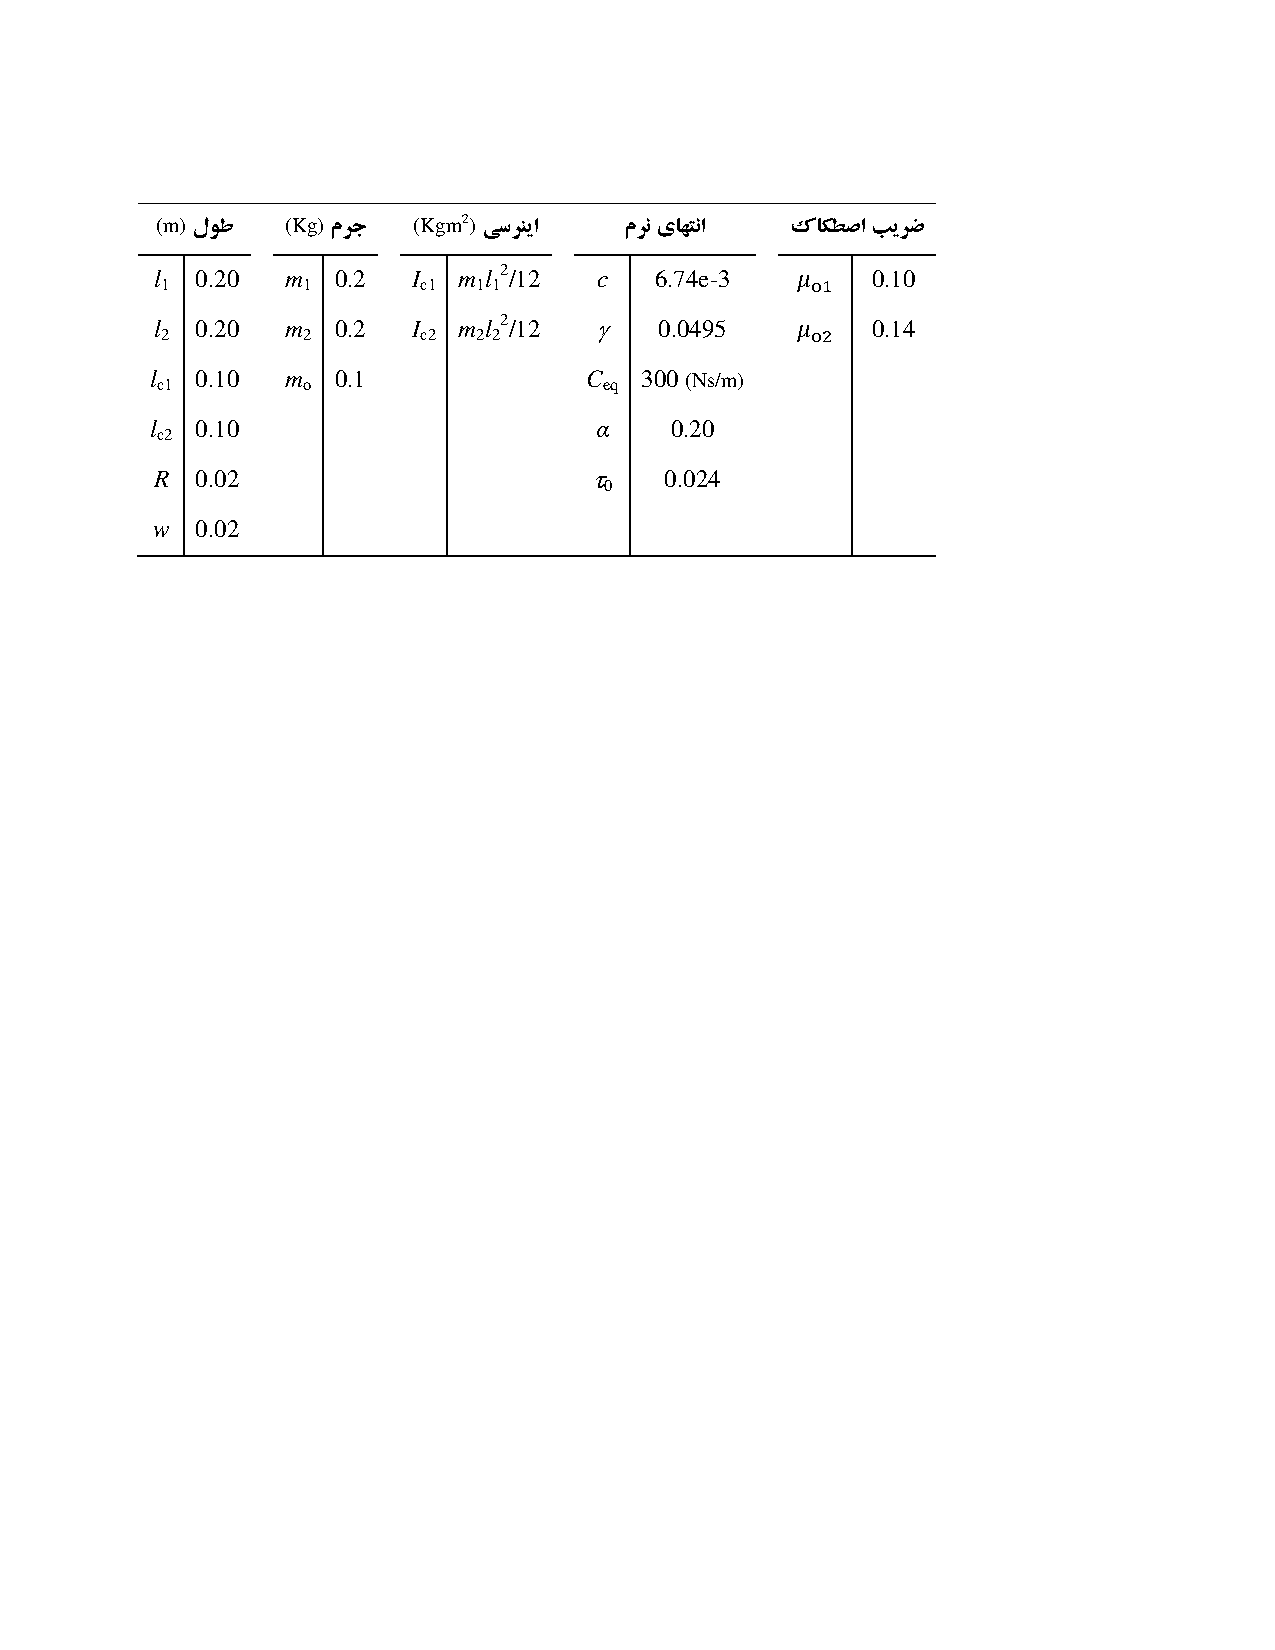
\includegraphics[scale=0.9]{Figures/SampleTable1.pdf} 
\end{tabular}
\vspace{-\baselineskip}
\label{Tbl:SampleTable1_2}
\end{table}

\begin{table}[!htb]
\caption{مقايسه‌ی روش‌هاي برداشت انرژي مبتني بر لرزش‌هاي مکانيکی}
\centering
\begin{tabular}{@{}|p{.15\textwidth}|p{.25\textwidth}|p{.25\textwidth}|p{.25\textwidth}|@{}}
\hline
روش
& 
چگالی انرژی
& 
ابعاد
& 
عیب اصلی
\\ \hline \hline
پیزوالکتریک
& 
$\mathrm{mJ/cm^3}$ 35/4
& 
بزرگ
& 
ولتاژ خروجی کم
\\ \hline
الکترومغناطیس
& 
$\mathrm{mJ/cm^3}$ 24/8
& 
بزرگ
& 
ولتاژ خروجی بسیار کم
\\ \hline
الکترواستاتیک
& 
$\mathrm{mJ/cm^3}$ 4
& 
فشرده در تراشه‌ها
& 
نیاز به منبع شارژ اولیه
\\ \hline
\end{tabular}
\label{Tbl:SampleTable2_2}
\vspace{-\baselineskip}
\end{table}

نمونه‌ای از یک رابطه به‌صورت
\begin{equation}
p\left( r \right) = {C_k}\frac{N}{{\pi {a^2}}}{\left[{1 - {{\left( {\frac{r}{a}} \right)}^k}} \right]^{\frac{1}{k}}},
\label{Eq:Pressure_2}
\end{equation}
است. در رابطه
\ref{Eq:Pressure_2}،
$N$
نیروی عمودی است. نمونه‌ای از استفاده از روابط متوالی به‌صورت
\begin{equation}
\sum \limits_{i = 1}^{k + 1} {E_s}\left( i \right) - T \sum \limits_{i = 1}^k {P_s}\left( i \right) \le B_s^{max},\quad k = 1, \ldots ,N - 1,
\label{Eq:batterysource_2}
\end{equation}\vspace{-\baselineskip}
\begin{equation}
\sum \limits_{i = 1}^{k + 1} {E_r}\left( i \right) - T \sum \limits_{i = 1}^k {P_r}\left( i \right) \le B_r^{max},\quad k = 1, \ldots ,N - 1,
\label{Eq:batteryrellay_2}
\end{equation}
است. نمونه‌ای از یک قضیه و تبصره نیز در ادامه آورده شده است.
\begin{theorem}
اگر ظرفیت باتری‌ها به اندازه کافی بزرگ باشد، جواب بهینه‌ی 
$P_s^*(i)$
و
$P_r^*(i)$
وجود دارد به نحوی که تابع هدف را بیشینه می‌کند و در رابطه‌ی زیر صدق می‌کند:
\begin{equation}
C\left( {{{\left| {{h_{sr}}\left( i \right)} \right|}^2}{P_s}^*\left( i \right)} \right) \ge C\left( {{{\left| {{h_{sd}}\left( i \right)} \right|}^2}{P_s}^*\left( i \right)} \right) + C\left( {{{\left| {{h_{rd}}\left( {i + 1} \right)} \right|}^2}P_r^*\left( {i} \right)} \right).
\label{Eq:theorem1_2}
\end{equation}

\begin{proof}
بار دیگر فرم تابع هدف را در نظر می‌گیریم. لازم به ذکر است اینجا تابع هدف یک تابع دومتغیره است.
\begin{equation}
{R({\mathbf{P}_s},{\mathbf{P}_r}) = {\frac{1}{2}\sum\limits_{i = 1}^N {\min } \left\{ {C\left( {{{\left| {{h_{sr}}\left( i \right)} \right|}^2}{P_s}\left( i \right)} \right),} C\left( {{{\left| {{h_{sd}}\left( i \right)} \right|}^2}{P_s}\left( i \right)} \right) \right\} }}.
\end{equation}
حال بلوک
$i$ام
را در نظر می‌گیریم. اگر رابطه‌ی
\ref{Eq:theorem1_2}
برای
$i$
برقرار نباشد، به عبارت دیگر اگر داشته باشیم،
\begin{equation}
C\left( {{{\left| {{h_{sr}}\left( i \right)} \right|}^2}{P_s}^*\left( i \right)} \right) < C\left( {{{\left| {{h_{sd}}\left( i \right)} \right|}^2}{P_s}^*\left( i \right)} \right) + C\left( {{{\left| {{h_{rd}}\left( {i + 1} \right)} \right|}^2}P_r^*\left( {i + 1} \right)} \right),
\label{Eq:theorem1(2)_2}
\end{equation}
بنابراین
\begin{equation}
C\left( {{{\left| {{h_{sr}}\left( i \right)} \right|}^2}{P_s}^*\left( i \right)} \right)+ C\left( {{{\left| {{h_{sd}}\left( i \right)} \right|}^2}{P_s}^*\left( i \right)} \right) =C\left( {{{\left| {{h_{sr}}\left( i \right)} \right|}^2}{P_s}^*\left( i \right)} \right).
\end{equation}
پس در تابع هدف مسئله، مقدار بهینه‌ی مسئله برابر عبارت سمت چپ رابطه‌ی
\ref{Eq:theorem1(2)_2}
شده است و آرگومان دوم و  هم‌چنین مقدار
$P_r^*(i)$
هیچ نقشی در مقدار بهینه ندارد. بنابراین می‌توانیم 
$P_r^*(i)$
را آنقدر کاهش دهیم تا در رابطه‌ی
\ref{Eq:theorem1(2)_2}
تساوی برقرار شود بدون آنکه مقدار بهینه‌ی مسئله تغییر کند.
\end{proof}
\label{theorem1_2}
\end{theorem}

\begin{remark}
از قضیه‌ی
\ref{theorem1_2}
نتیجه می‌گیریم که جواب بهینه‌ی مسئله‌ی
\lr{P}
در حالت کلی یکتا نیست. به طور مثال وقتی مقدار انرژی برداشت‌شده در رله خیلی بیشتر از این انرژی در منبع باشد مسئله می‌تواند جواب‌های زیادی داشته باشد. بنابراین همواره می‌توان برای صرفه‌جویی در مصرف انرژی، بدون کاهش مقدار نرخ گذردهی سیستم، کمترین مقدار توان را برای رله انتخاب کرد. بنابراین با توجه به رابطه
\begin{equation}
C\left( {{{\left| {{h_{sr}}\left( i \right)} \right|}^2}{P_s}^*\left( i \right)} \right) 
\ge C\left( {{{\left| {{h_{sd}}\left( i \right)} \right|}^2}{P_s}^*\left( i \right)} \right) + C\left( {{{\left| {{h_{rd}}\left( {i} \right)} \right|}^2}P_r^*\left( {i} \right)} \right),
\label{Eq:remark1_2}
\end{equation}
و با  استفاده از رابطه
\ref{Eq:remark1_2}
خواهیم داشت،
\begin{equation}
{R_r}(i) = \min \left\{ {C\left( {{{\left| {{h_{rd}}(i)} \right|}^2}{P_r}(i)} \right),C\left( {{{\left| {{h_{sr}}(i)} \right|}^2}{P_s}(i)} \right)} \right\}.
\end{equation}

بنابراین می‌توان با انتخاب کمترین توان و نرخ برای رله از مصرف بی‌رویه‌ی انرژی جلوگیری کرد. فرض بزرگ بودن ظرفیت باتری‌ به این دلیل است که اگر ظرفیت باتری محدود باشد برای کاهش
$P_r^*(i)$
با محدودیت مواجه هستیم. چون در صورت کاهش بی از حد توان رله ممکن است از ناحیه‌ی شدنی مسئله خارج شویم. به هر حال برای هر دو حالت ظرفیت نامحدود و محدود باتری جواب مسئله یکتا نیست و همواره می‌توان با کاهش توان رله مصرف انرژی را کاهش داد.
\end{remark}










%% !TEX root = ../ui-thesis.tex
% !TeX program = xelatex

\chapter{نتیجه‌گیری و پیشنهادها}
\section{‌نتیجه‌گیری}
نوشته نمونه نوشته نمونه نوشته نمونه نوشته نمونه نوشته نمونه نوشته نمونه نوشته نمونه نوشته نمونه نوشته نمونه نوشته نمونه نوشته نمونه نوشته نمونه نوشته نمونه نوشته نمونه نوشته نمونه نوشته نمونه نوشته نمونه نوشته نمونه نوشته نمونه نوشته نمونه نوشته نمونه نوشته نمونه. نوشته نمونه نوشته نمونه نوشته نمونه نوشته نمونه نوشته نمونه نوشته نمونه نوشته نمونه نوشته نمونه نوشته نمونه نوشته نمونه نوشته نمونه نوشته نمونه نوشته نمونه نوشته نمونه نوشته نمونه نوشته نمونه نوشته نمونه نوشته نمونه نوشته نمونه نوشته نمونه نوشته نمونه نوشته نمونه. نوشته نمونه نوشته نمونه نوشته نمونه نوشته نمونه نوشته نمونه نوشته نمونه نوشته نمونه نوشته نمونه نوشته نمونه نوشته نمونه نوشته نمونه نوشته نمونه نوشته نمونه نوشته نمونه نوشته نمونه نوشته نمونه نوشته نمونه نوشته نمونه نوشته نمونه نوشته نمونه نوشته نمونه نوشته نمونه. نوشته نمونه نوشته نمونه نوشته نمونه نوشته نمونه نوشته نمونه نوشته نمونه نوشته نمونه نوشته نمونه نوشته نمونه نوشته نمونه نوشته نمونه نوشته نمونه نوشته نمونه نوشته نمونه نوشته نمونه نوشته نمونه نوشته نمونه نوشته نمونه نوشته نمونه نوشته نمونه نوشته نمونه نوشته نمونه. نوشته نمونه نوشته نمونه نوشته نمونه نوشته نمونه نوشته نمونه نوشته نمونه نوشته نمونه نوشته نمونه نوشته نمونه نوشته نمونه نوشته نمونه نوشته نمونه نوشته نمونه نوشته نمونه نوشته نمونه نوشته نمونه نوشته نمونه نوشته نمونه نوشته نمونه نوشته نمونه نوشته نمونه نوشته نمونه. نوشته نمونه نوشته نمونه نوشته نمونه نوشته نمونه نوشته نمونه نوشته نمونه نوشته نمونه نوشته نمونه نوشته نمونه نوشته نمونه نوشته نمونه نوشته نمونه نوشته نمونه نوشته نمونه نوشته نمونه نوشته نمونه نوشته نمونه نوشته نمونه نوشته نمونه نوشته نمونه نوشته نمونه نوشته نمونه. نوشته نمونه نوشته نمونه نوشته نمونه نوشته نمونه نوشته نمونه نوشته نمونه نوشته نمونه نوشته نمونه نوشته نمونه نوشته نمونه نوشته نمونه نوشته نمونه نوشته نمونه نوشته نمونه نوشته نمونه نوشته نمونه نوشته نمونه نوشته نمونه نوشته نمونه نوشته نمونه نوشته نمونه نوشته نمونه.

\section{پیشنهادها}
نوشته نمونه نوشته نمونه نوشته نمونه نوشته نمونه نوشته نمونه نوشته نمونه نوشته نمونه نوشته نمونه نوشته نمونه نوشته نمونه نوشته نمونه نوشته نمونه نوشته نمونه نوشته نمونه نوشته نمونه نوشته نمونه نوشته نمونه نوشته نمونه نوشته نمونه نوشته نمونه نوشته نمونه نوشته نمونه. نوشته نمونه نوشته نمونه نوشته نمونه نوشته نمونه نوشته نمونه نوشته نمونه نوشته نمونه نوشته نمونه نوشته نمونه نوشته نمونه نوشته نمونه نوشته نمونه نوشته نمونه نوشته نمونه نوشته نمونه نوشته نمونه نوشته نمونه نوشته نمونه نوشته نمونه نوشته نمونه نوشته نمونه نوشته نمونه. نوشته نمونه نوشته نمونه نوشته نمونه نوشته نمونه نوشته نمونه نوشته نمونه نوشته نمونه نوشته نمونه نوشته نمونه نوشته نمونه نوشته نمونه نوشته نمونه نوشته نمونه نوشته نمونه نوشته نمونه نوشته نمونه نوشته نمونه نوشته نمونه نوشته نمونه نوشته نمونه نوشته نمونه نوشته نمونه. نوشته نمونه نوشته نمونه نوشته نمونه نوشته نمونه نوشته نمونه نوشته نمونه نوشته نمونه نوشته نمونه نوشته نمونه نوشته نمونه نوشته نمونه نوشته نمونه نوشته نمونه نوشته نمونه نوشته نمونه نوشته نمونه نوشته نمونه نوشته نمونه نوشته نمونه نوشته نمونه نوشته نمونه نوشته نمونه. نوشته نمونه نوشته نمونه نوشته نمونه نوشته نمونه نوشته نمونه نوشته نمونه نوشته نمونه نوشته نمونه نوشته نمونه نوشته نمونه نوشته نمونه نوشته نمونه نوشته نمونه نوشته نمونه نوشته نمونه نوشته نمونه نوشته نمونه نوشته نمونه نوشته نمونه نوشته نمونه نوشته نمونه نوشته نمونه. نوشته نمونه نوشته نمونه نوشته نمونه نوشته نمونه نوشته نمونه نوشته نمونه نوشته نمونه نوشته نمونه نوشته نمونه نوشته نمونه نوشته نمونه نوشته نمونه نوشته نمونه نوشته نمونه نوشته نمونه نوشته نمونه نوشته نمونه نوشته نمونه نوشته نمونه نوشته نمونه نوشته نمونه نوشته نمونه. نوشته نمونه نوشته نمونه نوشته نمونه نوشته نمونه نوشته نمونه نوشته نمونه نوشته نمونه نوشته نمونه نوشته نمونه نوشته نمونه نوشته نمونه نوشته نمونه نوشته نمونه نوشته نمونه نوشته نمونه نوشته نمونه نوشته نمونه نوشته نمونه نوشته نمونه نوشته نمونه نوشته نمونه نوشته نمونه.
%\input{Chapters/Chapter4}
%\input{Chapters/Chapter5}
%\input{Chapters/Chapter6}

% ░░░░░░░▒▒▒▒▒▒▓▓▓▓ References ▓▓▓▓▒▒▒▒▒▒░░░░░░░
\MakeReferences
\bibliographystyle{Settings/ieeetr-fa}
\bibliography{References}

 ----------------------------------------------------------------------------
%\clearpage
\pagestyle{myheadings}
%\pagenumbering{arabic}
%\setcounter{page}{1}

% ░░░░░░░▒▒▒▒▒▒▓▓▓▓ Chapters ▓▓▓▓▒▒▒▒▒▒░░░░░░░
%\clearpage
%\baselineskip=0.9cm
\linespread{1.0} % single-line spacing
%\linespread{1.3} % one and a half line spacing
%\linespread{1.6} % double-line spacing

\settextfont[Scale=1.2, ItalicFont=*, ItalicFeatures={FakeSlant=0.32}, BoldItalicFont=* Bold, BoldItalicFeatures={FakeSlant=0.32}]{B Nazanin}
\titleformat{\chapter}[display]
{\fontsize{15pt}{0}\selectfont  \flushleft  \bfseries \BNazaninScaleOne} % B Nazanin 15
{\chaptertitlename\ \tartibi{chapter}}{0.3cm}{\fontsize{15pt}{0}\selectfont \BNazaninScaleOne} % B Nazanin 15

\sectionfont{\fontsize{14pt}{\baselineskip}\selectfont \bfseries \BNazaninScaleOne} % B Nazanin 14
\subsectionfont{\fontsize{13pt}{\baselineskip}\selectfont \bfseries \BNazaninScaleOne} % B Nazanin 13
\subsubsectionfont{\fontsize{13pt}{\baselineskip}\selectfont \bfseries \BNazaninScaleOne} % B Nazanin 13

%\titlespacing*{\chapter}{0pt}{3.5cm}{8cm}
\titlespacing*{\section}{0pt}{1.2\baselineskip}{0pt}
\titlespacing*{\subsection}{0pt}{1.1\baselineskip}{0pt}
\titlespacing*{\subsubsection}{0pt}{1\baselineskip}{0pt}

\makeatletter
\renewcommand\chapter{\if@openright\cleardoublepage\else\clearpage\fi
	%\thispagestyle{empty}
	\global\@topnum\z@
	\@afterindentfalse
	\secdef\@chapter\@schapter}
\makeatother

% ░░░░░░░▒▒▒▒▒▒▓▓▓▓ Appendices ▓▓▓▓▒▒▒▒▒▒░░░░░░░
\MakeAppendices
\addtocontents{lof}{\protect\setcounter{tocdepth}{0}} % ignore adding appendix figures to list of figures
\addtocontents{lot}{\protect\setcounter{tocdepth}{0}} % ignore adding appendix table to list of tables
\captionsetup{list=no}

\section{جزئیات معادله‌ها}
نوشته نمونه نوشته نمونه نوشته نمونه نوشته نمونه نوشته نمونه نوشته نمونه نوشته نمونه نوشته نمونه نوشته نمونه نوشته نمونه نوشته نمونه نوشته نمونه نوشته نمونه نوشته نمونه نوشته نمونه نوشته نمونه نوشته نمونه نوشته نمونه نوشته نمونه نوشته نمونه نوشته نمونه نوشته نمونه. نوشته نمونه نوشته نمونه نوشته نمونه نوشته نمونه نوشته نمونه نوشته نمونه نوشته نمونه نوشته نمونه نوشته نمونه نوشته نمونه نوشته نمونه نوشته نمونه نوشته نمونه نوشته نمونه نوشته نمونه نوشته نمونه نوشته نمونه نوشته نمونه نوشته نمونه نوشته نمونه نوشته نمونه نوشته نمونه. نوشته نمونه نوشته نمونه نوشته نمونه نوشته نمونه نوشته نمونه نوشته نمونه نوشته نمونه نوشته نمونه نوشته نمونه نوشته نمونه نوشته نمونه نوشته نمونه نوشته نمونه نوشته نمونه نوشته نمونه نوشته نمونه نوشته نمونه نوشته نمونه نوشته نمونه نوشته نمونه نوشته نمونه نوشته نمونه. نوشته نمونه نوشته نمونه نوشته نمونه نوشته نمونه نوشته نمونه نوشته نمونه نوشته نمونه نوشته نمونه نوشته نمونه نوشته نمونه نوشته نمونه نوشته نمونه نوشته نمونه نوشته نمونه نوشته نمونه نوشته نمونه نوشته نمونه نوشته نمونه نوشته نمونه نوشته نمونه نوشته نمونه نوشته نمونه. نوشته نمونه نوشته نمونه نوشته نمونه نوشته نمونه نوشته نمونه نوشته نمونه نوشته نمونه نوشته نمونه نوشته نمونه نوشته نمونه نوشته نمونه نوشته نمونه نوشته نمونه نوشته نمونه نوشته نمونه نوشته نمونه نوشته نمونه نوشته نمونه نوشته نمونه نوشته نمونه نوشته نمونه نوشته نمونه. نوشته نمونه نوشته نمونه نوشته نمونه نوشته نمونه نوشته نمونه نوشته نمونه نوشته نمونه نوشته نمونه نوشته نمونه نوشته نمونه نوشته نمونه نوشته نمونه نوشته نمونه نوشته نمونه نوشته نمونه نوشته نمونه نوشته نمونه نوشته نمونه نوشته نمونه نوشته نمونه نوشته نمونه نوشته نمونه. نوشته نمونه نوشته نمونه نوشته نمونه نوشته نمونه نوشته نمونه نوشته نمونه نوشته نمونه نوشته نمونه. نمونه‌ای از یک رابطه به‌صورت
\begin{equation}
p\left( r \right) = {C_k}\frac{N}{{\pi {a^2}}}{\left[{1 - {{\left( {\frac{r}{a}} \right)}^k}} \right]^{\frac{1}{k}}}
\label{Eq:Pressure1}
\end{equation}
است.

\newpage
\section{اثبات روابط ریاضی}
نوشته نمونه نوشته نمونه نوشته نمونه نوشته نمونه نوشته نمونه نوشته نمونه نوشته نمونه نوشته نمونه نوشته نمونه نوشته نمونه نوشته نمونه نوشته نمونه نوشته نمونه نوشته نمونه نوشته نمونه نوشته نمونه نوشته نمونه نوشته نمونه نوشته نمونه نوشته نمونه نوشته نمونه نوشته نمونه. نوشته نمونه نوشته نمونه نوشته نمونه نوشته نمونه نوشته نمونه نوشته نمونه نوشته نمونه نوشته نمونه نوشته نمونه نوشته نمونه نوشته نمونه نوشته نمونه نوشته نمونه نوشته نمونه نوشته نمونه نوشته نمونه نوشته نمونه نوشته نمونه نوشته نمونه نوشته نمونه نوشته نمونه نوشته نمونه. نوشته نمونه نوشته نمونه نوشته نمونه نوشته نمونه نوشته نمونه نوشته نمونه نوشته نمونه نوشته نمونه نوشته نمونه نوشته نمونه نوشته نمونه نوشته نمونه نوشته نمونه نوشته نمونه نوشته نمونه نوشته نمونه نوشته نمونه نوشته نمونه نوشته نمونه نوشته نمونه نوشته نمونه نوشته نمونه. (شکل~%
\ref{Fig:World1})
نوشته نمونه نوشته نمونه نوشته نمونه نوشته نمونه نوشته نمونه نوشته نمونه نوشته نمونه نوشته نمونه نوشته نمونه نوشته نمونه نوشته نمونه نوشته نمونه نوشته نمونه نوشته نمونه نوشته نمونه نوشته نمونه نوشته نمونه نوشته نمونه نوشته نمونه نوشته نمونه نوشته نمونه نوشته نمونه. نوشته نمونه نوشته نمونه نوشته نمونه نوشته نمونه نوشته نمونه نوشته نمونه نوشته نمونه نوشته نمونه نوشته نمونه نوشته نمونه نوشته نمونه نوشته نمونه نوشته نمونه نوشته نمونه نوشته نمونه نوشته نمونه نوشته نمونه نوشته نمونه نوشته نمونه نوشته نمونه نوشته نمونه نوشته نمونه. نوشته نمونه نوشته نمونه نوشته نمونه نوشته نمونه نوشته نمونه نوشته نمونه نوشته نمونه نوشته نمونه نوشته نمونه نوشته نمونه نوشته نمونه نوشته نمونه نوشته نمونه نوشته نمونه نوشته نمونه نوشته نمونه نوشته نمونه نوشته نمونه نوشته نمونه نوشته نمونه نوشته نمونه نوشته نمونه.
\begin{figure}[!htb]
\centering
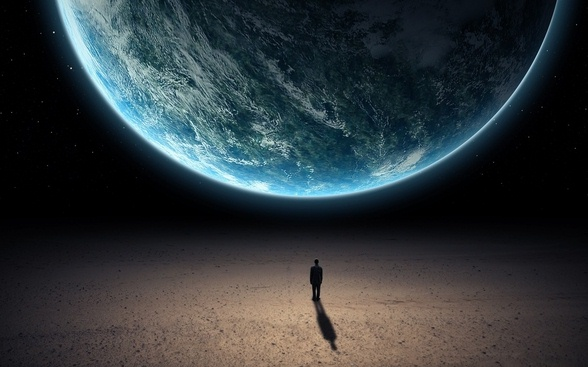
\includegraphics[scale=0.4]{Figures/World.jpg}
\caption{تصویر مفهومی}
\label{Fig:World1}
\end{figure}

نوشته نمونه نوشته نمونه نوشته نمونه نوشته نمونه نوشته نمونه نوشته نمونه نوشته نمونه نوشته نمونه نوشته نمونه نوشته نمونه نوشته نمونه نوشته نمونه نوشته نمونه نوشته نمونه نوشته نمونه نوشته نمونه نوشته نمونه نوشته نمونه نوشته نمونه نوشته نمونه نوشته نمونه نوشته نمونه.

% ░░░░░░░▒▒▒▒▒▒▓▓▓▓ Dictionary ▓▓▓▓▒▒▒▒▒▒░░░░░░░
\onehalfspacing
% !TEX root = ../ui-thesis.tex
% !TeX program = xelatex

\chapter*{واژه‌نامه فارسی به انگلیسی}\markboth{واژه‌نامه فارسی به انگلیسی}{واژه‌نامه فارسی به انگلیسی}
\addcontentsline{toc}{chapter}{واژه‌نامه فارسی به انگلیسی}
\thispagestyle{empty}
\noindent
\persiangloss{تضاد}{Conflict}
\persiangloss{ناسازگاری}{Incoherency}
\persiangloss{سازگاری}{Coherency}
\persiangloss{تناقض}{Inconsistency}
\persiangloss{آنتولوژی}{Ontology}
\persiangloss{گزاره}{Axiom}
\persiangloss{منطق توصیفی}{Description Logics}
\persiangloss{اعلانی}{Assertional}
\persiangloss{واژگانی}{Terminological}
\persiangloss{مشخصه‌سازی}{Specification}
\persiangloss{مصداق‌ناپذیری}{Unsatisfiability}
\persiangloss{بازنمایی}{Representation}
\persiangloss{سرمفهوم}{Top Concept}
\persiangloss{ته‌مفهوم}{‌Bottom Concept}
\persiangloss{تراگذری}{Transitivity}
\persiangloss{گزاره کلاس مجزا}{Class Disjointness Axiom}

% ░░░░░░░▒▒▒▒▒▒▓▓▓▓ Abstract - English ▓▓▓▓▒▒▒▒▒▒░░░░░░░
% !TEX root = ../ui-thesis.tex
% !TeX program = xelatex

\AbstractEn{
Lorem ipsum dolor sit amet, consectetur adipiscing elit, sed do eiusmod tempor incididunt ut labore et dolore magna aliqua. Duis at tellus at urna. Egestas sed sed risus pretium quam vulputate. Urna duis convallis convallis tellus id interdum velit laoreet id. Arcu non odio euismod lacinia at. Pharetra convallis posuere morbi leo urna molestie at elementum. Urna molestie at elementum eu facilisis. Pharetra massa massa ultricies mi quis hendrerit dolor magna. Amet consectetur adipiscing elit duis tristique sollicitudin. Malesuada pellentesque elit eget gravida cum sociis natoque. Cursus euismod quis viverra nibh cras pulvinar mattis nunc. Diam in arcu cursus euismod. Id velit ut tortor pretium viverra suspendisse potenti nullam ac. Risus ultricies tristique nulla aliquet. Egestas fringilla phasellus faucibus scelerisque. Id eu nisl nunc mi.
Luctus accumsan tortor posuere ac ut consequat semper viverra. Ut venenatis tellus in metus vulputate eu. Morbi tristique senectus et netus et. Dignissim enim sit amet venenatis urna. Ac turpis egestas integer eget aliquet nibh praesent. Consectetur libero id faucibus nisl tincidunt eget nullam non. Metus aliquam eleifend mi in nulla. Eget aliquet nibh praesent tristique magna. Nunc consequat interdum varius sit. Nisi quis eleifend quam adipiscing vitae. Odio eu feugiat pretium nibh ipsum consequat nisl. Dolor sit amet consectetur adipiscing elit. Viverra orci sagittis eu volutpat odio facilisis. Mauris nunc congue nisi vitae suscipit tellus. Elit eget gravida cum sociis natoque. Massa tincidunt nunc pulvinar sapien et. Purus viverra accumsan in nisl nisi scelerisque eu ultrices. In arcu cursus euismod quis. Suspendisse in est ante in nibh mauris cursus mattis.
}

\KeywordsEn{1- First Keyword, 2- Second Keyword, 3- Third Keyword, 4- Fourth Keyword, 5- Fifth Keyword}

\MakeEnglishAbstract

% ░░░░░░░▒▒▒▒▒▒▓▓▓▓ Signature - English ▓▓▓▓▒▒▒▒▒▒░░░░░░░
\DepartmentEn{Faculty of Computer Engineering}
\DegreeEn{Ph.D.} % Or \DegreeEn{M.Sc.)} 
\YourFullnameEn{Student First and Last Name}
\DateEn{Month Year} %
\FirstSupervisorEn{Supervisor First and Last Name}
%\SecondSupervisorEn{Second Supervisor, Prof.} % Optional (Remove It If You Don't Have)
\TitleEn{Thesis English Title} 
%\\[0.2cm] second line (if any)} %% Break the title, if required
% اگر عنوان رساله طولانی بود، در دو خط به صورت نشان داده شده تقسیم شود.
\GroupEn{Department of Software Engineering}
\FirstAdvisorEn{First Advisor, Assoc. Prof.}

\MakeEnglishSignaturePage

\end{document} 

